%%==========================================================================
%% This is the very first version of a Streetwise LaTeX template. By
%% chosing the document class, it is easily convertible to a two-column IEEE
%% paper format, provided any conflicting packages and (new)commmands are
%% removed.
%%
%% Erwin de Gelder, January 6, 2018
%%==========================================================================

%%==========================================================================
%% Title:
%% Author(s):
%% To be published in:
%% Date of submission:
%% Date of submission R1:
%% Date of submission R2:
%% Date of final submission:
%%==========================================================================


%% Generic
\documentclass[10pt,final,a4paper,oneside,onecolumn]{article}

%% IEEE
%% Document class options: replace "draftcls" by "final" for final document.
%% All other options may just as well be omitted because they are the default values.
%\documentclass[10pt,final,journal,letterpaper,twoside,twocolumn]{IEEEtran}


%%==========================================================================
%% Document automation
%%==========================================================================

\def\reptitle{Hyperparameter selection for scenario generation}
\def\repauthor{Erwin de Gelder, etc.}


%%==========================================================================
%% Packages
%%==========================================================================

\usepackage[a4paper,left=3.5cm,right=3.5cm,top=3cm,bottom=3cm]{geometry} %% change page layout; remove for IEEE paper format
\usepackage[T1]{fontenc}                        %% output font encoding for international characters (e.g., accented)
\usepackage[cmex10]{amsmath}                    %% math typesetting; consider using the [cmex10] option
\usepackage{amssymb}                            %% special (symbol) fonts for math typesetting
\usepackage{amsthm}                             %% theorem styles
\usepackage{dsfont}                             %% double stroke roman fonts: the real numbers R: $\mathds{R}$
\usepackage{mathrsfs}                           %% formal script fonts: the Laplace transform L: $\mathscr{L}$
\usepackage[pdftex]{graphicx}                   %% graphics control; use dvips for TeXify; use pdftex for PDFTeXify
\usepackage{array}                              %% array functionality (array, tabular)
\usepackage{upgreek}                            %% upright Greek letters; add the prefix 'up', e.g. \upphi
\usepackage[noadjust]{cite}                     %% citations; noadjust removes leading spaces
%\usepackage[round]{natbib}                     %% Author-year citations (remove package cite)
\usepackage{stfloats}                           %% improved handling of floats
\usepackage{multirow}                           %% cells spanning multiple rows in tables
%\usepackage{subfigure}                         %% subfigures and corresponding captions (for use with IEEEconf.cls)
\usepackage{subfig}                             %% subfigures (IEEEtran.cls: set caption=false)
\usepackage{fancyhdr}                           %% page headers and footers
\usepackage[official,left]{eurosym}             %% the euro symbol; command: \euro
\usepackage{appendix}                           %% appendix layout
\usepackage{xspace}                             %% add space after macro depending on context
\usepackage{verbatim}                           %% provides the comment environment
\usepackage[dutch,USenglish]{babel}             %% language support
\usepackage{wrapfig}                            %% wrapping text around figures
\usepackage{longtable}                          %% tables spanning multiple pages
%\usepackage[utf8]{inputenc}
\usepackage{pgfplots}                           %% support for TikZ figures (Matlab)
\usepackage[breaklinks=true,hidelinks,          %% implement hyperlinks (dvips yields minor problems with breaklinks;
            bookmarksnumbered=true]{hyperref}   %% IEEEtran: set bookmarks=false)
%\usepackage[hyphenbreaks]{breakurl}            %% allow line breaks in URLs (don't use with PDFTeX)
\usepackage{lmodern} 
\usepackage{etoolbox}							%% Needed for apptocmd later

%%==========================================================================
%% Fancy headers and footers
%%==========================================================================

\pagestyle{fancy}                                       %% set page style
\fancyhf{}                                              %% clear all header & footer fields
\fancyhead[L]{
\includegraphics[width=15mm]{Streetwise}} %% define headers (LE: left field/even pages, etc.)
\fancyhead[R]{\small\emph{\reptitle}}                   %% similar
\fancyfoot[C]{\thepage}                                 %% define footer
\setlength{\headheight}{18pt}                           %% increase head height to accommodate an oversized picture in the header
\renewcommand*{\headrulewidth}{0.25pt}                  %% header line width
\renewcommand*{\footrulewidth}{0pt}                     %% footer line width
%% Redefine the default "plain" page style (automatically activated by \maketitle, \section, ...)
\fancypagestyle{plain}{\fancyhf{}
                       \fancyhead[C]{
\includegraphics[width=30mm]{Streetwise}}
                       \renewcommand{\headrulewidth}{0pt}
                       \renewcommand{\footrulewidth}{0pt}
                       \setlength{\headheight}{36pt}}


%%==========================================================================
%% TikZ figures
%%==========================================================================

\newlength\figurewidth
\setlength\figurewidth{0.35\textwidth}              %% set figure height
\newlength\figureheight
\setlength\figureheight{0.3\textwidth}              %% set figure width
\pgfplotsset{every axis/.append style={
    scaled y ticks=false,
    scaled x ticks=false,
    y tick label style={/pgf/number format/fixed},
    x tick label style={/pgf/number format/fixed},
    legend style={font=\small}},
    compat=1.9}                                     %% PGFPlots package options
\usetikzlibrary{arrows}                             %% plot arrows
\usetikzlibrary{external}                           %% Create pdf figures from TikZ. Use PDFTeXify ...
\tikzexternalize[prefix=./tikz/]                    %% ... with --tex-option=--shell-escape switch.
%\tikzset{external/force remake}                    %% force pdf figure update


%%==========================================================================
%% User-defined commands
%%==========================================================================

\newcommand*{\mat}[1]{\mathbf{#1}}                              %% matrix/vector notation
\newcommand*{\matsym}[1]{\boldsymbol{#1}}                       %% matrix/vector notation for Greek letters
\newcommand*{\T}{^{\scriptscriptstyle\mathsf{T}}}               %% transpose operator
\newcommand*{\Hr}{^{\scriptscriptstyle\mathsf{H}}}              %% conjugate transpose operator
\newcommand*{\ud}{\mathrm{\,d}}                                 %% differential operator (upright d)
\newcommand*{\defeq}{\mathrel{\mathop:}=}                       %% definition sign :=
\newcommand*{\eqdef}{=\mathrel{\mathop:}}                       %% definition sign =:
\newcommand*{\ip}[2]{\left\langle#1\,{,}\,#2\right\rangle}      %% inner product
\newcommand*{\real}[1]{\mathrm{Re}(#1)}                         %% real part
\newcommand*{\imag}[1]{\mathrm{Im}(#1)}                         %% imaginary part
\newcommand*{\lsup}[1]{{}^{#1}\!}                               %% left superscript
\newcommand*{\hi}[1]{$^\text{#1}$}                              %% superscript in normal text
\newcommand*{\lo}[1]{$_\text{#1}$}                              %% subscript in normal text
\newcommand*{\w}[1]{\mathrm{#1}}                                %% multiple character super-/subscript in math mode
\newcommand*{\Ln}{{\ensuremath{\mathcal{L}}}\xspace}            %% L norm
\newcommand*{\Lone}{{\ensuremath{\mathcal{L}_1}}\xspace}        %% L_1 norm
\newcommand*{\Ltwo}{{\ensuremath{\mathcal{L}_2}}\xspace}        %% L_2 norm
\newcommand*{\Linf}{{\ensuremath{\mathcal{L}_\infty}}\xspace}   %% L_inf norm
\newcommand*{\Lp}{{\ensuremath{\mathcal{L}_p}}\xspace}          %% L_p norm
\newcommand*{\Htwo}{{\ensuremath{\mathcal{H}_2}}\xspace}        %% H_2 norm
\newcommand*{\Hinf}{{\ensuremath{\mathcal{H}_\infty}}\xspace}   %% H_inf norm
\newcommand*{\Hp}{{\ensuremath{\mathcal{H}_p}}\xspace}          %% H_p norm
\newcommand*{\capskip}{\vspace{-12pt}}                          %% caption skip for figures with subfloats
\newcommand*{\etal}{et al.}                                     %% may be required for Natbib bibliography styles
\renewcommand*{\qedsymbol}{$\blacksquare$}                      %% redefine the end-of-proof symbol
\renewcommand*{\labelitemi}{$\bullet$}                          %% first level item list bullet
\renewcommand*{\labelitemii}{$-$}                               %% second level item list bullet
%\renewcommand*{\theenumi}{\textit{\roman{enumi}}}               %% first level enumerator
\renewcommand*{\labelenumi}{\theenumi.}
\renewcommand*{\theenumii}{\textit{\alph{enumii}}}              %% second level enumerator
\renewcommand*{\labelenumii}{\theenumii.}
\DeclareMathOperator{\tr}{tr}                                   %% trace of a matrix
\DeclareMathOperator{\sgn}{sgn}                                 %% signum function
\DeclareMathOperator{\atan}{atan}                               %% arc tangent


%%==========================================================================
%% User-defined environments
%%==========================================================================

\theoremstyle{plain}\newtheorem{definition}{Definition}[section]    %% definition
                    \newtheorem{theorem}{Theorem}[section]          %% theorem
                    \newtheorem{lemma}[theorem]{Lemma}              %% lemma
                    \newtheorem{corollary}[theorem]{Corollary}      %% corollary
                    \newtheorem{assumption}{Assumption}[section]    %% assumption
                    \newtheorem{condition}{Condition}[section]      %% condition
\theoremstyle{definition}\newtheorem{example}{Example}[section]     %% examples
\theoremstyle{remark}\newtheorem{remarkenv}{Remark}[section]        %% remarks
\newenvironment{remark}{\begin{remarkenv}}%
                       {\hfill$\blacklozenge$\end{remarkenv}}       %% end remark with a lozenge
\newenvironment{reviewer}{\itshape}{\upshape}                       %% environment for reviewer's comments


%%==========================================================================
%% Miscellaneous
%%==========================================================================

\graphicspath{{./../}{./figures/}{./more_figures/}} %% (graphicx) directory path for figures
%\setlength{\parindent}{0pt}                        %% no paragraph indentation
%\setlength{\parskip}{2ex}                          %% create empty line between paragraphs
%\interdisplaylinepenalty=2500                      %% (amsmath) allow for page breaks within multiline equations
%\numberwithin{equation}{section}                   %% (amsmath) include section number in equation numbering
%\numberwithin{figure}{section}                     %% (amsmath) include section number in figure numbering
%\numberwithin{table}{section}                      %% (amsmath) include section number in table numbering
\addtolength{\arraycolsep}{-0.5mm}                  %% squeeze matrix columns a little
\fnbelowfloat                                       %% (stfloats) put footnote below a float at the page bottom
\urlstyle{same}                                     %% (hyperref) use current font for URLs
\hypersetup{pdftitle={\reptitle},
            pdfauthor={\repauthor}}                 %% (hyperref) pdf properties title and author
%\raggedbottom                                      %% don't add inter-paragraph spacing to achieve \textheight
%\setlength\subfigcapskip{-3pt}                     %% (subfigure) distance between subfloat and subcaption
%\setlength\subfigbottomskip{-3pt}                  %% (subfigure) distance between subcaption and caption
%\renewcommand*{\subcapsize}{\small}                %% (subfigure) subcaption font size
\renewcommand*{\thesubfigure}{(\alph{subfigure})}   %% (subfig) implement 1(a) instead of 1a ...as subfigure reference
\captionsetup[subfloat]{labelformat=simple}        %% ... as subfigure reference
%\captionsetup[subfloat]{
%    farskip=0pt,
%    nearskip=8pt,
%    captionskip=1.5pt,
%    labelfont={small,bf},
%    textfont=small}                                %% (subfig) subfloat caption format
%\captionsetup[figure]{
%    labelfont={small,bf},
%    textfont=small}                                %% (subfig/caption) figure caption format
%\captionsetup[table]{
%    aboveskip=2pt,
%    labelfont={small,bf},
%    textfont={small,sc}}                           %% (subfig/caption) table caption format
\bibliographystyle{IEEEtran}                        %% (BibTeX) references style, e.g., IEEEtran, plainnat, abbrvnat, unsrtnat, or thesisnat
\apptocmd{\thebibliography}{\raggedright}{}{}		%% Suppress badness warnings in bibliography


%%==========================================================================
%% Begin document
%%==========================================================================

\begin{document}

\selectlanguage{USenglish}

\title{\textbf{\reptitle}}
\author{\repauthor}
\date{\today}
\maketitle

\tableofcontents

\newpage

\section{Introduction}

For the generation of test scenarios for the performance assessment of Automated Vehicles (AVs), it is important to generate realistic trajectories of vehicles. Real-life data could be used to generate realistic trajectories \cite{deGelder2017assessment}. In Figure~\ref{fig:velocity example}a, an example of a velocity profile from real-life driving data is shown. The recorded trajectories from the real-life data need to be parametrized, such that probability density functions (PDFs) can be estimated. From these estimation PDFs, new parameters can be generated. These generated parameters are then used to generate a trajectory. 

\begin{figure}[b]
	\begin{center}
		\setlength\figureheight{150pt}
		\setlength\figurewidth{0.49\linewidth}
		\subfloat[Original]{% This file was created by matplotlib2tikz v0.6.14.
\begin{tikzpicture}

\definecolor{color3}{rgb}{0.83921568627451,0.152941176470588,0.156862745098039}
\definecolor{color2}{rgb}{0.172549019607843,0.627450980392157,0.172549019607843}
\definecolor{color1}{rgb}{1,0.498039215686275,0.0549019607843137}
\definecolor{color0}{rgb}{0.12156862745098,0.466666666666667,0.705882352941177}

\begin{axis}[
xlabel={Time [s]},
ylabel={Velocity [km/h]},
xmin=-0.405, xmax=8.505,
ymin=-0.128527297559858, ymax=50.9958346332171,
width=\figurewidth,
height=\figureheight,
tick align=outside,
tick pos=left,
xmajorgrids,
x grid style={white!69.019607843137251!black},
ymajorgrids,
y grid style={white!69.019607843137251!black},
legend cell align={left},
legend entries={{Profile 1},{Profile 2},{Profile 3},{Profile 4}},
legend style={draw=white!80.0!black}
]
\addlegendimage{no markers, color0}
\addlegendimage{no markers, color1}
\addlegendimage{no markers, color2}
\addlegendimage{no markers, color3}
\addplot [semithick, color0, mark=*, mark size=1, mark options={solid}, only marks]
table {%
0 48.672
0.1 48.6359918994937
0.2 47.9159878492406
0.3 47.375962482237
0.4 46.4759661771686
0.5 45.5398532671499
0.6 44.567824915378
0.7 43.4157646613031
0.8 42.29969559451
0.9 41.2916970126468
1 39.9956646106218
1.1 38.8618378493623
1.2 37.5478254838316
1.3 36.4676637612536
1.4 35.1716329227879
1.5 34.0015198318347
1.6 32.8674551343703
1.7 31.4097739319247
1.8 29.9876879204179
1.9 28.7453026814198
2 27.467341656224
2.1 26.2253887315345
2.2 24.9472728019208
2.3 23.471640170536
2.4 22.3550563713891
2.5 20.6271142735906
2.6 19.295333982059
2.7 17.8910381809574
2.8 16.5229428943627
2.9 15.1007890808964
3 13.7507984249087
3.1 12.2935431385527
3.2 10.9075264803432
3.3 9.8270245995681
3.4 8.78306794438217
3.5 7.84696789602428
3.6 6.87493954425236
3.7 5.81345310924209
3.8 4.78727862860074
3.9 3.83293169244461
4 2.98698956843009
4.1 2.19530733565728
};
\addplot [semithick, color1, mark=*, mark size=1, mark options={solid}, only marks]
table {%
0 47.088
0.1 46.9079863570422
0.2 46.7999676690327
0.3 46.5479802461338
0.4 46.3679702254707
0.5 46.1159598531504
0.6 45.9358601596821
0.7 45.4498142231174
0.8 45.179940454173
0.9 44.729704544694
1 44.3158188044651
1.1 43.8836856435103
1.2 43.3796156522959
1.3 42.767789955294
1.4 42.0838333001078
1.5 41.5075281810371
1.6 40.8955037374065
1.7 40.2294110079255
1.8 39.5993835088374
1.9 38.8795685414562
2 37.9797001391539
2.1 37.3852946164394
2.2 36.68367427438
2.3 35.9631533633361
2.4 35.3150331264124
2.5 34.5051798318338
2.6 33.6233394534536
2.7 32.9032192325912
2.8 32.111495850071
2.9 31.4444417183995
3 30.4553562229219
3.1 29.9144526054014
3.2 29.2667486138953
3.3 28.3131804140041
3.4 27.5397595428659
3.5 26.8006419351036
3.6 26.2428597471555
3.7 25.5592204405501
3.8 24.8025352295064
3.9 24.0298637835918
4 23.3986030116011
4.1 22.6793546660349
4.2 21.9596708636399
4.3 21.4004881897229
4.4 20.7706317250088
4.5 20.2666044390949
4.6 19.6907574960284
4.7 19.1152763547719
4.8 18.5036320664783
4.9 17.9985009799961
5 17.5308574022717
5.1 17.0268369378363
5.2 16.4870142531641
5.3 15.8930926011825
5.4 15.299260445287
5.5 14.7406843782999
5.6 14.1466629901203
5.7 13.5526391149456
5.8 12.958617726766
5.9 12.453991216557
6 11.8423685296134
6.1 11.1595853109241
6.2 10.4393688000234
6.3 9.80807570341702
6.4 9.21361447195764
6.5 8.53068047016063
6.6 7.84599002842424
6.7 7.10886806083318
6.8 6.44308081477942
6.9 5.81190431375665
7 5.14634863363259
7.1 4.56960679779292
7.2 3.92181861892924
7.3 3.2390168543433
7.4 2.51875579065799
};
\addplot [semithick, color2, mark=*, mark size=1, mark options={solid}, only marks]
table {%
0 48.672
0.1 48.608995283563
0.2 48.455994244377
0.3 48.1499559446157
0.4 48.0239525338739
0.5 47.7179552340439
0.6 47.4119101119168
0.7 47.0879575785089
0.8 46.6558044509344
0.9 46.1519450018259
1 45.6478472272915
1.1 45.2157983400267
1.2 44.8197433393213
1.3 44.3876808084788
1.4 43.9557843417831
1.5 43.6319079801829
1.6 43.0918501391549
1.7 42.6235759313898
1.8 42.1916050647879
1.9 41.651644213726
2 41.0034997582104
2.1 40.5357376572865
2.2 39.9237254327615
2.3 39.2933547307219
2.4 38.6992524722155
2.5 38.0150641691167
2.6 37.4394314723628
2.7 36.773082805036
2.8 36.0714011250792
2.9 35.2613784931797
3 34.5953583483032
3.1 33.785335716398
3.2 33.1913130912778
3.3 32.5071905178296
3.4 32.2546217634148
3.5 31.2471259893812
3.6 30.4914375832673
3.7 29.8430756895968
3.8 29.2670512366027
3.9 28.6192701017491
4 28.1511270552457
4.1 27.5027206047803
4.2 26.9273441432204
4.3 26.4231946391366
4.4 25.8835881532068
4.5 25.4154386491253
4.6 24.8389962378834
4.7 24.2806803505508
4.8 23.7949509844374
4.9 23.2190825110755
5 22.6078440297254
5.1 22.1208868199009
5.2 21.6710147129051
5.3 21.1306604188455
5.4 20.6268052463816
5.5 20.033131327285
5.6 19.4392928330335
5.7 18.8985612363945
5.8 18.3587172066642
5.9 17.7468831849665
6 17.1702956961133
6.1 16.5410378872341
6.2 15.8750226003189
6.3 15.3352051477411
6.4 14.6869920454748
6.5 14.1281662850803
6.6 13.4985585362236
6.7 12.9769551057457
6.8 12.3463037088183
6.9 11.6991396409641
7 11.0151274105371
7.1 10.3302289560398
7.2 9.6455292745252
7.3 8.87149566453292
7.4 8.0259234991623
7.5 7.19859733338512
7.6 6.37057898663801
7.7 5.52335924441851
7.8 4.71343313430595
7.9 3.90339952431368
8 3.20136591431246
8.1 2.37502992884368
};
\addplot [semithick, color3, mark=*, mark size=1, mark options={solid}, only marks]
table {%
0 30.492
0.1 30.3839935337426
0.2 30.0959935337426
0.3 29.7719418036832
0.4 29.411922404911
0.5 28.9439030061386
0.6 28.4038254110494
0.7 27.719954736198
0.8 27.0358189447921
0.9 26.3157090184159
1 25.6315473619803
1.1 24.8756443558417
1.2 24.1555732312219
1.3 23.4355796932674
1.4 22.715502103092
1.5 21.9058545092079
1.6 21.1317930715936
1.7 20.4113233878768
1.8 19.6554038252768
1.9 18.9894343445907
2 18.3954052464323
2.1 17.6397227325662
2.2 17.0278549000257
};
\end{axis}

\end{tikzpicture}}
		\subfloat[Normalized]{% This file was created by matplotlib2tikz v0.6.16.
\begin{tikzpicture}

\definecolor{color0}{rgb}{0.12156862745098,0.466666666666667,0.705882352941177}

\begin{axis}[
xlabel={Normalized time},
ylabel={Normalized velocity},
xmin=-0.05, xmax=1.05,
ymin=-0.05, ymax=1.05,
width=\figurewidth,
height=\figureheight,
tick align=outside,
tick pos=left,
xmajorgrids,
x grid style={white!69.01960784313725!black},
ymajorgrids,
y grid style={white!69.01960784313725!black}
]
\addplot [semithick, color0, forget plot]
table {%
0 0.985915492957746
0.00680274027029168 1
0.0136054805405858 0.987323943661972
0.0204082208108775 0.988732394366197
0.0272110282176721 0.987323943661972
0.0340137684879662 0.991549295774648
0.0408165087582578 0.988732394366197
0.0476192490285519 0.987323943661972
0.0544219892988436 0.980281690140845
0.0612247295691377 0.98169014084507
0.0680274698394294 0.977464788732394
0.0748302101097235 0.970422535211268
0.0816329503800152 0.963380281690141
0.0884356906503093 0.957746478873239
0.095238430920601 0.947887323943662
0.102043319558936 0.940845070422535
0.115648800099522 0.929577464788732
0.122451540369816 0.919718309859155
0.129254280640107 0.916901408450704
0.136057020910402 0.902816901408451
0.142859761180693 0.894366197183099
0.149662501450987 0.890140845070422
0.156465241721279 0.87887323943662
0.163267981991573 0.863380281690141
0.170070722261865 0.856338028169014
0.176873462532159 0.849295774647887
0.183676202802451 0.835211267605634
0.190478943072745 0.828169014084507
0.197281683343036 0.814084507042254
0.20408442361333 0.802816901408451
0.210887163883622 0.794366197183099
0.217689904153916 0.784507042253521
0.224492644424208 0.774647887323944
0.231295384694502 0.763380281690141
0.238098124964794 0.746478873239437
0.244900865235088 0.740845070422535
0.251703672641882 0.725352112676056
0.258506412912174 0.714084507042253
0.265309153182468 0.704225352112676
0.27211189345276 0.691549295774648
0.278914633723054 0.67887323943662
0.285717373993346 0.670422535211267
0.292517965895596 0.659154929577465
0.299320706165891 0.64225352112676
0.306123446436182 0.638028169014084
0.312926119569973 0.623943661971831
0.319728926976768 0.609859154929577
0.326531667247062 0.598591549295775
0.333334407517354 0.588732394366197
0.340137147787648 0.574647887323944
0.34693988805794 0.563380281690141
0.353742628328234 0.552112676056338
0.360545368598525 0.538028169014084
0.367348108868819 0.530985915492958
0.374150849139111 0.519718309859155
0.380953589409405 0.501408450704225
0.394559069949991 0.485915492957746
0.401361810220283 0.470422535211268
0.408164550490577 0.461971830985915
0.414967290760868 0.446478873239437
0.421770031031163 0.436619718309859
0.428572771301454 0.430985915492958
0.435375511571748 0.419718309859155
0.44217825184204 0.408450704225352
0.448980992112334 0.401408450704225
0.455783732382626 0.390140845070422
0.46258647265292 0.37887323943662
0.469389212923212 0.373239436619718
0.476191953193506 0.361971830985915
0.482994693463797 0.352112676056338
0.489797433734091 0.349295774647887
0.496600174004383 0.340845070422535
0.503402914274677 0.332394366197183
0.517008394815263 0.325352112676056
0.523811135085555 0.32112676056338
0.530613875355849 0.322535211267606
0.53741661562614 0.315492957746479
0.551020149208187 0.312676056338028
0.557822889478481 0.308450704225352
0.564625629748773 0.305633802816901
0.571428370019067 0.302816901408451
0.578231110289358 0.297183098591549
0.591836590829944 0.295774647887324
0.598639331100238 0.290140845070422
0.612244811640824 0.285915492957746
0.619047551911116 0.283098591549296
0.62585029218141 0.28169014084507
0.632653032451702 0.280281690140845
0.639455772721996 0.274647887323944
0.653061253262581 0.267605633802817
0.659863993532876 0.261971830985915
0.673469474073461 0.257746478873239
0.680272214343753 0.249295774647887
0.687074954614047 0.250704225352113
0.693877694884339 0.242253521126761
0.700680435154633 0.236619718309859
0.707483175424925 0.229577464788732
0.714285915695219 0.225352112676056
0.72108865596551 0.22112676056338
0.727891396235804 0.219718309859155
0.734694136506096 0.212676056338028
0.74149687677639 0.205633802816901
0.748299617046682 0.204225352112676
0.755102357316976 0.195774647887324
0.761905097587268 0.190140845070423
0.768707837857562 0.184507042253521
0.775510578127853 0.177464788732394
0.782313318398147 0.171830985915493
0.789116058668439 0.167605633802817
0.795918798938733 0.164788732394366
0.802721539209025 0.154929577464789
0.809524279479319 0.150704225352113
0.816327019749611 0.142253521126761
0.823129760019905 0.136619718309859
0.829932500290196 0.133802816901408
0.836735240560491 0.129577464788732
0.843537980830782 0.125352112676056
0.850340721101076 0.11830985915493
0.857142454323848 0.109859154929577
0.863945194594142 0.107042253521127
0.870747934864434 0.102816901408451
0.877550675134728 0.0943661971830986
0.88435341540502 0.0915492957746479
0.891156155675314 0.0845070422535211
0.897958895945606 0.0774647887323944
0.9047616362159 0.0746478873239437
0.911564376486191 0.0690140845070423
0.918367116756485 0.0605633802816902
0.925169857026777 0.0577464788732394
0.931972597297071 0.0492957746478873
0.938775337567363 0.0422535211267606
0.945578077837657 0.0394366197183099
0.952380818107949 0.0323943661971831
0.959183558378243 0.0267605633802817
0.965986298648534 0.0225352112676056
0.972789038918828 0.0169014084507042
0.97959177918912 0.0112676056338028
0.986394519459414 0.00845070422535212
0.993197259729706 0.00140845070422538
1 0
};
\end{axis}

\end{tikzpicture}}
		\caption{Example of a velocity profile from real-life driving data.}
		\label{fig:velocity example}
	\end{center}
\end{figure}

In the process of going from real-life driving data to the generation of new trajectories, there are many choices to be made. For example, how should the parametrization be performed? How should the PDFs be estimated? To answer these questions, it would be useful to have a measure that objectively measures how good these choices are. This document describes such a method.

\section{Method}

When tuning the hyperparameters for a specific model, often the data is split into a training and a test set, such that the training set is used to fit a model, while the test set is used to ``measure'' how good the fitted model fits the test data. One approach for measuring how good the model fits the test data, is by determining the likelihood that the test data would have been generated by the model. The higher the likelihood, the better the model fits to the test data. In case of the trajectories, there is a problem with this method, because the recorded trajectories cannot be exactly reproduces due to the parametrization. 

Because the likelihood cannot be used, another method is introduced. The first step is to normalize the time and velocity, such that they are on the domain $[0, 1]$. See Figure~\ref{fig:velocity example} for an example. Let $y_i$ with $i=\{1,\ldots,n\}$ be the test samples. Next, $z$ is a sample from the PDF $p(Z)$. The score $J$ is defined as follows:
\begin{equation}
	J = \prod_{i=1}^n \int f(z,y_i)p(z)dz = \prod_{i=1}^n E[f(z,y_i)].
\end{equation}

Here, $f(z,y_i)$ is the so-called error function and $E[\cdot]$ denotes the expectation. The main question is how to define $f(z,y_i)$, because it is not obvious how $z$ and $y_i$ should be compared. There is one case, however, when it 

\section{Simple case}

\begin{figure}
	\begin{center}
		\setlength\figureheight{200pt}
		\setlength\figurewidth{300pt}
		% This file was created by matplotlib2tikz v0.6.16.
\begin{tikzpicture}

\begin{axis}[
xlabel={t},
ylabel={y},
xmin=-0.05, xmax=1.05,
ymin=-0.05, ymax=1.05,
width=\figurewidth,
height=\figureheight,
tick align=outside,
tick pos=left,
xmajorgrids,
x grid style={white!69.01960784313725!black},
ymajorgrids,
y grid style={white!69.01960784313725!black},
legend style={draw=white!80.0!black},
legend entries={{Training curve},{Test curve}},
legend cell align={left}
]
\addlegendimage{no markers, blue}
\addlegendimage{no markers, red}
\addplot [semithick, blue]
table {%
0 1
0.0526315789473684 0.997229916897507
0.105263157894737 0.988919667590028
0.157894736842105 0.975069252077562
0.210526315789474 0.955678670360111
0.263157894736842 0.930747922437673
0.315789473684211 0.900277008310249
0.368421052631579 0.864265927977839
0.421052631578947 0.822714681440443
0.473684210526316 0.775623268698061
0.526315789473684 0.722991689750693
0.578947368421053 0.664819944598338
0.631578947368421 0.601108033240997
0.684210526315789 0.531855955678671
0.736842105263158 0.457063711911357
0.789473684210526 0.376731301939058
0.842105263157895 0.290858725761773
0.894736842105263 0.199445983379502
0.947368421052632 0.102493074792244
1 0
};
\addplot [semithick, blue, forget plot]
table {%
0 1
0.0526315789473684 0.897506925207756
0.105263157894737 0.800554016620499
0.157894736842105 0.709141274238227
0.210526315789474 0.623268698060942
0.263157894736842 0.542936288088643
0.315789473684211 0.46814404432133
0.368421052631579 0.398891966759003
0.421052631578947 0.335180055401662
0.473684210526316 0.277008310249307
0.526315789473684 0.224376731301939
0.578947368421053 0.177285318559557
0.631578947368421 0.135734072022161
0.684210526315789 0.0997229916897507
0.736842105263158 0.0692520775623269
0.789473684210526 0.0443213296398892
0.842105263157895 0.0249307479224377
0.894736842105263 0.0110803324099723
0.947368421052632 0.00277008310249305
1 0
};
\addplot [semithick, red]
table {%
0 1
0.0526315789473684 0.947368421052632
0.105263157894737 0.894736842105263
0.157894736842105 0.842105263157895
0.210526315789474 0.789473684210526
0.263157894736842 0.736842105263158
0.315789473684211 0.684210526315789
0.368421052631579 0.631578947368421
0.421052631578947 0.578947368421053
0.473684210526316 0.526315789473684
0.526315789473684 0.473684210526316
0.578947368421053 0.421052631578947
0.631578947368421 0.368421052631579
0.684210526315789 0.315789473684211
0.736842105263158 0.263157894736842
0.789473684210526 0.210526315789474
0.842105263157895 0.157894736842105
0.894736842105263 0.105263157894737
0.947368421052632 0.0526315789473685
1 0
};
\end{axis}

\end{tikzpicture}
		\caption{Simple example. The goal is to generate new curves using the two training curves, such that there is a chance of generated a curve that closely ``matches'' the test curve.}
	\end{center}
\end{figure}

\begin{figure}
	\begin{center}
		\setlength\figureheight{100pt}
		\setlength\figurewidth{0.3\linewidth}
		\subfloat[$h=0.01$]{% This file was created by matplotlib2tikz v0.6.14.
\begin{tikzpicture}

\definecolor{color0}{rgb}{0.5,0.5,1}

\begin{axis}[
xlabel={t},
ylabel={y},
xmin=-0.05, xmax=1.05,
ymin=-0.0499999999999967, ymax=1.05,
width=\figurewidth,
height=\figureheight,
tick align=outside,
tick pos=left,
xmajorgrids,
x grid style={white!69.019607843137251!black},
ymajorgrids,
y grid style={white!69.019607843137251!black}
]
\addplot [semithick, color0, forget plot]
table {%
0 1
0.0526315789473684 0.997196490117162
0.105263157894737 0.988832297944864
0.157894736842105 0.974912543607379
0.210526315789474 0.955442347228981
0.263157894736842 0.930426828933944
0.315789473684211 0.89987110884654
0.368421052631579 0.863780307091043
0.421052631578947 0.822159543791727
0.473684210526316 0.775013939072865
0.526315789473684 0.722348493793364
0.578947368421053 0.664165465708698
0.631578947368421 0.600464369470914
0.684210526315789 0.531244600466687
0.736842105263158 0.456505554082697
0.789473684210526 0.37624662570562
0.842105263157895 0.290467210722135
0.894736842105263 0.199166704518919
0.947368421052632 0.102344502482649
1 3.66373598126302e-15
};
\addplot [semithick, color0, forget plot]
table {%
0 1
0.0526315789473684 0.997165262800357
0.105263157894737 0.988829247153885
0.157894736842105 0.97498676905468
0.210526315789474 0.955632644496837
0.263157894736842 0.93076168947445
0.315789473684211 0.900368719981617
0.368421052631579 0.864448552012431
0.421052631578947 0.822996001560988
0.473684210526316 0.776005884621383
0.526315789473684 0.723472959150524
0.578947368421053 0.665390648249975
0.631578947368421 0.601751040165963
0.684210526315789 0.532546165107524
0.736842105263158 0.457768053283696
0.789473684210526 0.377408734903516
0.842105263157895 0.291460240176019
0.894736842105263 0.199914599310244
0.947368421052632 0.102763842515227
1 3.99680288865056e-15
};
\addplot [semithick, color0, forget plot]
table {%
0 0.999999999999999
0.0526315789473684 0.89712406233305
0.105263157894737 0.799807622119072
0.157894736842105 0.70805473291014
0.210526315789474 0.62186944825833
0.263157894736842 0.541255821715716
0.315789473684211 0.466217906834373
0.368421052631579 0.396759757166378
0.421052631578947 0.332885426263804
0.473684210526316 0.274598967678727
0.526315789473684 0.221904440920251
0.578947368421053 0.174806042509115
0.631578947368421 0.133308105977698
0.684210526315789 0.0974149708154051
0.736842105263158 0.0671309765116433
0.789473684210526 0.0424604625558183
0.842105263157895 0.0234077684373358
0.894736842105263 0.00997723364560199
0.947368421052632 0.00217319767002255
1 3.5527136788005e-15
};
\addplot [semithick, color0, forget plot]
table {%
0 0.999999999999999
0.0526315789473684 0.897332128850915
0.105263157894737 0.800192663686041
0.157894736842105 0.708587590035589
0.210526315789474 0.622522893429773
0.263157894736842 0.542004559398804
0.315789473684211 0.467038573472897
0.368421052631579 0.397630921182264
0.421052631578947 0.333787588057118
0.473684210526316 0.275514559627671
0.526315789473684 0.22281775321445
0.578947368421053 0.175701517315177
0.631578947368421 0.134168631604776
0.684210526315789 0.0982218075484783
0.736842105263158 0.0678637566115194
0.789473684210526 0.0430971902591336
0.842105263157895 0.0239248199565548
0.894736842105263 0.0103493571690175
0.947368421052632 0.0023735133617554
1 3.10862446895044e-15
};
\addplot [semithick, color0, forget plot]
table {%
0 0.999999999999999
0.0526315789473684 0.897843036674868
0.105263157894737 0.80121816839313
0.157894736842105 0.710120129175608
0.210526315789474 0.624543653043123
0.263157894736842 0.5444834740165
0.315789473684211 0.469934326116559
0.368421052631579 0.400890943364124
0.421052631578947 0.337348059780016
0.473684210526316 0.279300409385059
0.526315789473684 0.226742740310671
0.578947368421053 0.179670125231986
0.631578947368421 0.138077961367855
0.684210526315789 0.101961660047726
0.736842105263158 0.0713166326010446
0.789473684210526 0.0461382903572584
0.842105263157895 0.0264220446458142
0.894736842105263 0.0121633067961591
0.947368421052632 0.00335748813773995
1 3.66373598126302e-15
};
\addplot [semithick, color0, forget plot]
table {%
0 0.999999999999999
0.0526315789473684 0.89758113111015
0.105263157894737 0.800686271474967
0.157894736842105 0.709316169435032
0.210526315789474 0.623471573330926
0.263157894736842 0.54315323150323
0.315789473684211 0.468361892292526
0.368421052631579 0.399098304039394
0.421052631578947 0.335363215084415
0.473684210526316 0.277157373768171
0.526315789473684 0.224481619958337
0.578947368421053 0.177338898645743
0.631578947368421 0.135734259944377
0.684210526315789 0.0996728454953196
0.736842105263158 0.0691597969396524
0.789473684210526 0.0442002559184562
0.842105263157895 0.0247993640728125
0.894736842105263 0.0109622630438017
0.947368421052632 0.00269409447250502
1 3.66373598126302e-15
};
\addplot [semithick, color0, forget plot]
table {%
0 0.999999999999999
0.0526315789473684 0.897644883212418
0.105263157894737 0.800812728543145
0.157894736842105 0.709502967095667
0.210526315789474 0.623715029973476
0.263157894736842 0.543448348280061
0.315789473684211 0.468702353118912
0.368421052631579 0.399476475593517
0.421052631578947 0.335770146807368
0.473684210526316 0.277582797863952
0.526315789473684 0.224913986992793
0.578947368421053 0.177766196322142
0.631578947368421 0.136144831878984
0.684210526315789 0.100055426816333
0.736842105263158 0.0695035142872079
0.789473684210526 0.0444946274446227
0.842105263157895 0.025034299441594
0.894736842105263 0.0111280634311373
0.947368421052632 0.00278145256626849
1 3.88578058618805e-15
};
\addplot [semithick, color0, forget plot]
table {%
0 0.999999999999999
0.0526315789473684 0.897334970336146
0.105263157894737 0.800200027814956
0.157894736842105 0.708601723803036
0.210526315789474 0.622546609666996
0.263157894736842 0.542041236773444
0.315789473684211 0.467092156488987
0.368421052631579 0.397705920180235
0.421052631578947 0.333889079213796
0.473684210526316 0.275648184956277
0.526315789473684 0.222989590842807
0.578947368421053 0.175915097884458
0.631578947368421 0.134421954668251
0.684210526315789 0.0985072118497239
0.736842105263158 0.0681679200844152
0.789473684210526 0.0434011300278636
0.842105263157895 0.024203892335608
0.894736842105263 0.0105732576631872
0.947368421052632 0.00250627666613934
1 3.33066907387547e-15
};
\addplot [semithick, color0, forget plot]
table {%
0 1
0.0526315789473684 0.997210744415899
0.105263157894737 0.988831597162345
0.157894736842105 0.974872416615398
0.210526315789474 0.955343061151116
0.263157894736842 0.930253389145559
0.315789473684211 0.899613258974786
0.368421052631579 0.863432529014856
0.421052631578947 0.821721057641828
0.473684210526316 0.774488703231762
0.526315789473684 0.721745224228535
0.578947368421053 0.663498080635872
0.631578947368421 0.599752434017343
0.684210526315789 0.530513346004335
0.736842105263158 0.455785878228237
0.789473684210526 0.375575092320438
0.842105263157895 0.289886049912327
0.894736842105263 0.198723812635292
0.947368421052632 0.102093442120721
1 3.77475828372553e-15
};
\addplot [semithick, color0, forget plot]
table {%
0 1
0.0526315789473684 0.997533798482779
0.105263157894737 0.989516553811532
0.157894736842105 0.975943922103073
0.210526315789474 0.956811559474214
0.263157894736842 0.932115122041771
0.315789473684211 0.901850265922557
0.368421052631579 0.866012647233385
0.421052631578947 0.82459792209107
0.473684210526316 0.777601746612426
0.526315789473684 0.725019819986285
0.578947368421053 0.666848832057897
0.631578947368421 0.603086463328935
0.684210526315789 0.533730437373088
0.736842105263158 0.458778477764044
0.789473684210526 0.378228308075493
0.842105263157895 0.292077651881125
0.894736842105263 0.200324232754628
0.947368421052632 0.102965774269691
1 3.5527136788005e-15
};
\addplot [semithick, color0, forget plot]
table {%
0 1
0.0526315789473684 0.997450459685465
0.105263157894737 0.989344687957716
0.157894736842105 0.975681975169165
0.210526315789474 0.956461611672222
0.263157894736842 0.9316828878193
0.315789473684211 0.90134509396281
0.368421052631579 0.865447520455165
0.421052631578947 0.823989457648775
0.473684210526316 0.776970195896052
0.526315789473684 0.724388915400138
0.578947368421053 0.666242262930934
0.631578947368421 0.602524351825107
0.684210526315789 0.533229185270052
0.736842105263158 0.458350766453162
0.789473684210526 0.377883098561832
0.842105263157895 0.291820184783457
0.894736842105263 0.200156028305431
0.947368421052632 0.102884632315148
1 3.77475828372553e-15
};
\addplot [semithick, color0, forget plot]
table {%
0 0.999999999999999
0.0526315789473684 0.897192964115691
0.105263157894737 0.79994833950272
0.157894736842105 0.708267544133909
0.210526315789474 0.622151995982078
0.263157894736842 0.54160311302005
0.315789473684211 0.466622313220646
0.368421052631579 0.397211014556687
0.421052631578947 0.333370635000996
0.473684210526316 0.275102592526393
0.526315789473684 0.222408419894845
0.578947368421053 0.175292290018629
0.631578947368421 0.133761015960338
0.684210526315789 0.0978215255717083
0.736842105263158 0.0674807467044743
0.789473684210526 0.0427456072103728
0.842105263157895 0.0236230349411389
0.894736842105263 0.0101199577485092
0.947368421052632 0.00224330348421853
1 3.33066907387547e-15
};
\addplot [semithick, color0, forget plot]
table {%
0 1
0.0526315789473684 0.996847286855679
0.105263157894737 0.988207417026845
0.157894736842105 0.974077232518982
0.210526315789474 0.954453575337576
0.263157894736842 0.929333287488113
0.315789473684211 0.898713210976076
0.368421052631579 0.862590187806951
0.421052631578947 0.820961059986224
0.473684210526316 0.77382266951938
0.526315789473684 0.721172042905194
0.578947368421053 0.66301044998812
0.631578947368421 0.599343403958293
0.684210526315789 0.530176602499136
0.736842105263158 0.455515743294073
0.789473684210526 0.375366524026528
0.842105263157895 0.289734642379925
0.894736842105263 0.198625796037687
0.947368421052632 0.102045682683239
1 3.77475828372553e-15
};
\addplot [semithick, color0, forget plot]
table {%
0 0.999999999999999
0.0526315789473684 0.897795485761563
0.105263157894737 0.801092671828385
0.157894736842105 0.709892636059032
0.210526315789474 0.624196456312071
0.263157894736842 0.544005210446067
0.315789473684211 0.469319976319586
0.368421052631579 0.400141831791195
0.421052631578947 0.33647185471946
0.473684210526316 0.278311122962947
0.526315789473684 0.225660721753509
0.578947368421053 0.178521905908618
0.631578947368421 0.136896099831363
0.684210526315789 0.10078473529812
0.736842105263158 0.0701892440852659
0.789473684210526 0.0451110579691771
0.842105263157895 0.0255516087262297
0.894736842105263 0.011512328132801
0.947368421052632 0.00299464796526661
1 3.66373598126302e-15
};
\addplot [semithick, color0, forget plot]
table {%
0 0.999999999999999
0.0526315789473684 0.897272151224103
0.105263157894737 0.8001551722145
0.157894736842105 0.708640193887714
0.210526315789474 0.622718347160271
0.263157894736842 0.542380762948693
0.315789473684211 0.467618572169506
0.368421052631579 0.398422905739234
0.421052631578947 0.3347848945744
0.473684210526316 0.276695669591529
0.526315789473684 0.224146502330938
0.578947368421053 0.177131898680175
0.631578947368421 0.13564959887402
0.684210526315789 0.0996974837710441
0.736842105263158 0.0692734342298201
0.789473684210526 0.0443753311089203
0.842105263157895 0.0250010552669165
0.894736842105263 0.0111484875623813
0.947368421052632 0.00281550885388615
1 3.99680288865056e-15
};
\addplot [semithick, color0, forget plot]
table {%
0 1
0.0526315789473684 0.997234185732072
0.105263157894737 0.988929155654706
0.157894736842105 0.975084548236603
0.210526315789474 0.955700001946469
0.263157894736842 0.930775155253005
0.315789473684211 0.900309646624916
0.368421052631579 0.864303114530905
0.421052631578947 0.822755197439675
0.473684210526316 0.775665533819929
0.526315789473684 0.723033777696331
0.578947368421053 0.66485994088063
0.631578947368421 0.601144392971659
0.684210526315789 0.531887519124212
0.736842105263158 0.457089704493084
0.789473684210526 0.376751334233068
0.842105263157895 0.290872793498958
0.894736842105263 0.199454467445548
0.947368421052632 0.102496741227632
1 3.5527136788005e-15
};
\addplot [semithick, color0, forget plot]
table {%
0 0.999999999999999
0.0526315789473684 0.897602759405501
0.105263157894737 0.800739634346932
0.157894736842105 0.709410566421132
0.210526315789474 0.623615497224942
0.263157894736842 0.543354368355202
0.315789473684211 0.46862712140875
0.368421052631579 0.399433697982428
0.421052631578947 0.335774039673074
0.473684210526316 0.277648088077528
0.526315789473684 0.225055678422506
0.578947368421053 0.177994199421851
0.631578947368421 0.136458593276535
0.684210526315789 0.100443695817406
0.736842105263158 0.0699443428753103
0.789473684210526 0.0449553702810963
0.842105263157895 0.0254716138656113
0.894736842105263 0.0114879094597026
0.947368421052632 0.00299909289421751
1 3.77475828372553e-15
};
\addplot [semithick, color0, forget plot]
table {%
0 0.999999999999999
0.0526315789473684 0.897086096669229
0.105263157894737 0.799692413312422
0.157894736842105 0.707830968264361
0.210526315789474 0.62151377985983
0.263157894736842 0.540752866433611
0.315789473684211 0.465560246320488
0.368421052631579 0.395947937855242
0.421052631578947 0.331927959372658
0.473684210526316 0.273512329207518
0.526315789473684 0.220713030817995
0.578947368421053 0.173541245500232
0.631578947368421 0.132007352388344
0.684210526315789 0.0961216957398365
0.736842105263158 0.0658946198122122
0.789473684210526 0.0413364688629765
0.842105263157895 0.0224575871496331
0.894736842105263 0.00926831892968705
0.947368421052632 0.00177900846064205
1 3.33066907387547e-15
};
\addplot [semithick, color0, forget plot]
table {%
0 1
0.0526315789473684 0.997575831480354
0.105263157894737 0.989587904709569
0.157894736842105 0.976034848248281
0.210526315789474 0.956915290657125
0.263157894736842 0.932227860496739
0.315789473684211 0.901971186327757
0.368421052631579 0.866143896710817
0.421052631578947 0.824744620206555
0.473684210526316 0.777771985375606
0.526315789473684 0.725224444482872
0.578947368421053 0.667096394991379
0.631578947368421 0.603378179562272
0.684210526315789 0.534059964560965
0.736842105263158 0.459131916352869
0.789473684210526 0.378584201303397
0.842105263157895 0.292406985777962
0.894736842105263 0.200590436141977
0.947368421052632 0.103124718760853
1 3.77475828372553e-15
};
\addplot [semithick, color0, forget plot]
table {%
0 0.999999999999999
0.0526315789473684 0.897774332950052
0.105263157894737 0.801038947333365
0.157894736842105 0.709798807881601
0.210526315789474 0.624058879326425
0.263157894736842 0.5438241263995
0.315789473684211 0.469099513832491
0.368421052631579 0.399890006357061
0.421052631578947 0.336200568704874
0.473684210526316 0.278036165607595
0.526315789473684 0.225401563331204
0.578947368421053 0.17829696343097
0.631578947368421 0.136718002751447
0.684210526315789 0.100660119671509
0.736842105263158 0.0701187525700269
0.789473684210526 0.0450893398258745
0.842105263157895 0.0255673198179233
0.894736842105263 0.0115481309250463
0.947368421052632 0.00302721152611551
1 3.5527136788005e-15
};
\addplot [semithick, color0, forget plot]
table {%
0 0.999999999999999
0.0526315789473684 0.897060140523467
0.105263157894737 0.799690522374323
0.157894736842105 0.707893716319929
0.210526315789474 0.621672293127652
0.263157894736842 0.541028823564853
0.315789473684211 0.465965878398897
0.368421052631579 0.396486028397148
0.421052631578947 0.332591844326969
0.473684210526316 0.274285896955724
0.526315789473684 0.221570881702985
0.578947368421053 0.17445236098911
0.631578947368421 0.132938764235244
0.684210526315789 0.0970386455147386
0.736842105263158 0.0667605589009455
0.789473684210526 0.0421130584672178
0.842105263157895 0.0231046982869073
0.894736842105263 0.00974403243336674
0.947368421052632 0.00203961497994776
1 3.10862446895044e-15
};
\addplot [semithick, color0, forget plot]
table {%
0 0.999999999999999
0.0526315789473684 0.896785679392124
0.105263157894737 0.79913099362577
0.157894736842105 0.707046394164579
0.210526315789474 0.620542332472189
0.263157894736842 0.539629260012241
0.315789473684211 0.464317628248374
0.368421052631579 0.394617888644228
0.421052631578947 0.330540492663443
0.473684210526316 0.272095891769658
0.526315789473684 0.219294573447125
0.578947368421053 0.172147853654189
0.631578947368421 0.130667876823287
0.684210526315789 0.0948668234074664
0.736842105263158 0.0647568738597768
0.789473684210526 0.040350208633267
0.842105263157895 0.0216590081809858
0.894736842105263 0.00869545295598229
0.947368421052632 0.00147172341130508
1 3.5527136788005e-15
};
\addplot [semithick, color0, forget plot]
table {%
0 1
0.0526315789473684 0.996978801490513
0.105263157894737 0.988359476154206
0.157894736842105 0.97415907476995
0.210526315789474 0.954394648116611
0.263157894736842 0.929083246973059
0.315789473684211 0.898241922118163
0.368421052631579 0.861887724330791
0.421052631578947 0.820037704389811
0.473684210526316 0.772708913074093
0.526315789473684 0.719918132938907
0.578947368421053 0.661675977396774
0.631578947368421 0.597986890717466
0.684210526315789 0.528855048947157
0.736842105263158 0.45428462813202
0.789473684210526 0.374279804318229
0.842105263157895 0.288844753551959
0.894736842105263 0.197983651879382
0.947368421052632 0.101700675346672
1 3.99680288865056e-15
};
\addplot [semithick, color0, forget plot]
table {%
0 1
0.0526315789473684 0.996993705347076
0.105263157894737 0.988488127663306
0.157894736842105 0.974480249765847
0.210526315789474 0.954967054471856
0.263157894736842 0.92994552459849
0.315789473684211 0.899412642962908
0.368421052631579 0.863365392382266
0.421052631578947 0.821800755673721
0.473684210526316 0.774715715654432
0.526315789473684 0.722107316469278
0.578947368421053 0.663974012800778
0.631578947368421 0.600315669869091
0.684210526315789 0.531132214222096
0.736842105263158 0.456423572407676
0.789473684210526 0.376189670973709
0.842105263157895 0.290430436468078
0.894736842105263 0.199145795438663
0.947368421052632 0.102335674433345
1 3.88578058618805e-15
};
\addplot [semithick, color0, forget plot]
table {%
0 0.999999999999999
0.0526315789473684 0.897950271578162
0.105263157894737 0.801399528800546
0.157894736842105 0.710346789679854
0.210526315789474 0.624791072228788
0.263157894736842 0.544731394460051
0.315789473684211 0.470166774386345
0.368421052631579 0.401096230020372
0.421052631578947 0.337518779374835
0.473684210526316 0.279433440462436
0.526315789473684 0.226839168581275
0.578947368421053 0.179733476593605
0.631578947368421 0.138112434925831
0.684210526315789 0.101972051289758
0.736842105263158 0.0713083333971872
0.789473684210526 0.0461172889599235
0.842105263157895 0.0263949256897699
0.894736842105263 0.0121372512985297
0.947368421052632 0.0033402734980067
1 3.77475828372553e-15
};
\addplot [semithick, color0, forget plot]
table {%
0 0.999999999999999
0.0526315789473684 0.897750966817011
0.105263157894737 0.801078288887627
0.157894736842105 0.709970530541606
0.210526315789474 0.624416256108707
0.263157894736842 0.544404029918686
0.315789473684211 0.469922416301303
0.368421052631579 0.400959979586316
0.421052631578947 0.337505284103483
0.473684210526316 0.279546894182562
0.526315789473684 0.227073411483326
0.578947368421053 0.180074296255901
0.631578947368421 0.138539867340761
0.684210526315789 0.102460480908397
0.736842105263158 0.0718264931293013
0.789473684210526 0.0466282601739629
0.842105263157895 0.0268561382128732
0.894736842105263 0.012500483416523
0.947368421052632 0.00355165195540297
1 3.66373598126302e-15
};
\addplot [semithick, color0, forget plot]
table {%
0 1
0.0526315789473684 0.997151326673758
0.105263157894737 0.988736948502865
0.157894736842105 0.974763028276943
0.210526315789474 0.955235728785614
0.263157894736842 0.930161212818503
0.315789473684211 0.899545643165232
0.368421052631579 0.863395182615423
0.421052631578947 0.821715993958699
0.473684210526316 0.774514239984683
0.526315789473684 0.721796067238427
0.578947368421053 0.663567248639858
0.631578947368421 0.599833183483773
0.684210526315789 0.530599254820404
0.736842105263158 0.455870845699977
0.789473684210526 0.375653339172723
0.842105263157895 0.289952118288869
0.894736842105263 0.198772566098646
0.947368421052632 0.102120065652281
1 3.5527136788005e-15
};
\addplot [semithick, color0, forget plot]
table {%
0 0.999999999999999
0.0526315789473684 0.897146359012634
0.105263157894737 0.799921027921855
0.157894736842105 0.708312482047765
0.210526315789474 0.622309196710466
0.263157894736842 0.541899647230062
0.315789473684211 0.467072308926653
0.368421052631579 0.397815657120343
0.421052631578947 0.334118167131235
0.473684210526316 0.275968314279429
0.526315789473684 0.223355003335572
0.578947368421053 0.176277016432761
0.631578947368421 0.134743013066551
0.684210526315789 0.098762082183039
0.736842105263158 0.0683433127283209
0.789473684210526 0.0434957936484927
0.842105263157895 0.0242286138896509
0.894736842105263 0.0105508623978912
0.947368421052632 0.00247162811931023
1 3.77475828372553e-15
};
\addplot [semithick, color0, forget plot]
table {%
0 0.999999999999999
0.0526315789473684 0.897473471000651
0.105263157894737 0.800440201379481
0.157894736842105 0.708910644760786
0.210526315789474 0.622895254768865
0.263157894736842 0.542404485028013
0.315789473684211 0.467448789162529
0.368421052631579 0.398038620796709
0.421052631578947 0.334184433554851
0.473684210526316 0.275896681061251
0.526315789473684 0.223185602205607
0.578947368421053 0.176056496981804
0.631578947368421 0.134509726487915
0.684210526315789 0.0985454370874121
0.736842105263158 0.0681637751437695
0.789473684210526 0.0433648870204594
0.842105263157895 0.0241489190809551
0.894736842105263 0.010516017688729
0.947368421052632 0.0024663292072542
1 3.5527136788005e-15
};
\addplot [semithick, color0, forget plot]
table {%
0 1
0.0526315789473684 0.996931579035314
0.105263157894737 0.988309705682722
0.157894736842105 0.974143428341625
0.210526315789474 0.954441795411422
0.263157894736842 0.929213855291513
0.315789473684211 0.898468656381298
0.368421052631579 0.862215247080176
0.421052631578947 0.820462675787549
0.473684210526316 0.773219990902815
0.526315789473684 0.72049612017479
0.578947368421053 0.662297216388851
0.631578947368421 0.598626657366937
0.684210526315789 0.529487700280403
0.736842105263158 0.454883602300602
0.789473684210526 0.374817620598889
0.842105263157895 0.289293012346618
0.894736842105263 0.198313034715145
0.947368421052632 0.101880944875822
1 3.99680288865056e-15
};
\addplot [semithick, color0, forget plot]
table {%
0 0.999999999999999
0.0526315789473684 0.897843516697199
0.105263157894737 0.801214136654545
0.157894736842105 0.7101079683629
0.210526315789474 0.624521120313127
0.263157894736842 0.544449700996088
0.315789473684211 0.469889818902645
0.368421052631579 0.400837582523662
0.421052631578947 0.33728910035
0.473684210526316 0.279240480872522
0.526315789473684 0.226687775634667
0.578947368421053 0.179625726389134
0.631578947368421 0.138047765097883
0.684210526315789 0.101947266775448
0.736842105263158 0.071317606436367
0.789473684210526 0.046152159095174
0.842105263157895 0.0264442997664055
0.894736842105263 0.0121874034645971
0.947368421052632 0.00337484520428477
1 3.77475828372553e-15
};
\addplot [semithick, color0, forget plot]
table {%
0 0.999999999999999
0.0526315789473684 0.897445951726974
0.105263157894737 0.800463089915292
0.157894736842105 0.709046301135194
0.210526315789474 0.623190471956923
0.263157894736842 0.542890488950719
0.315789473684211 0.468141238686824
0.368421052631579 0.398937607735481
0.421052631578947 0.33527448266693
0.473684210526316 0.277146750051412
0.526315789473684 0.224549414398482
0.578947368421053 0.177480192821842
0.631578947368421 0.135939515039348
0.684210526315789 0.0999279287081676
0.736842105263158 0.0694459814854674
0.789473684210526 0.0444942210284139
0.842105263157895 0.0250731949941742
0.894736842105263 0.0111834510399146
0.947368421052632 0.0028255368228024
1 3.99680288865056e-15
};
\addplot [semithick, color0, forget plot]
table {%
0 1
0.0526315789473684 0.997661044909199
0.105263157894737 0.989764892070814
0.157894736842105 0.976306217184487
0.210526315789474 0.957279695949862
0.263157894736842 0.93268000406658
0.315789473684211 0.902501817234286
0.368421052631579 0.866739811152621
0.421052631578947 0.825388661521229
0.473684210526316 0.778443044039753
0.526315789473684 0.725897616942988
0.578947368421053 0.667746636774226
0.631578947368421 0.603983958385259
0.684210526315789 0.534603419163031
0.736842105263158 0.459598856494485
0.789473684210526 0.378964107766563
0.842105263157895 0.292693010366212
0.894736842105263 0.200779401680372
0.947368421052632 0.103217119095989
1 3.77475828372553e-15
};
\addplot [semithick, color0, forget plot]
table {%
0 0.999999999999999
0.0526315789473684 0.897063212309168
0.105263157894737 0.799671962890264
0.157894736842105 0.707833499161259
0.210526315789474 0.621555068540125
0.263157894736842 0.540843918444833
0.315789473684211 0.465707296293355
0.368421052631579 0.396152449503663
0.421052631578947 0.332186625493728
0.473684210526316 0.273817071681522
0.526315789473684 0.221051106803519
0.578947368421053 0.173897689921762
0.631578947368421 0.13236742042386
0.684210526315789 0.0964709690159275
0.736842105263158 0.0662190064040766
0.789473684210526 0.0416222032944207
0.842105263157895 0.0226912303930724
0.894736842105263 0.00943675840614466
0.947368421052632 0.0018694580397508
1 3.77475828372553e-15
};
\addplot [semithick, color0, forget plot]
table {%
0 1
0.0526315789473684 0.997193365044346
0.105263157894737 0.988871733600864
0.157894736842105 0.975030683299899
0.210526315789474 0.955665791771794
0.263157894736842 0.930772636646892
0.315789473684211 0.900346795555537
0.368421052631579 0.864383846128072
0.421052631578947 0.82287936599484
0.473684210526316 0.775828932786187
0.526315789473684 0.723228222651155
0.578947368421053 0.665075177668924
0.631578947368421 0.601370005848803
0.684210526315789 0.532113013718803
0.736842105263158 0.457304507806936
0.789473684210526 0.376944794641214
0.842105263157895 0.291034180749648
0.894736842105263 0.199572972660251
0.947368421052632 0.102561476901032
1 3.5527136788005e-15
};
\addplot [semithick, color0, forget plot]
table {%
0 0.999999999999999
0.0526315789473684 0.897213299033219
0.105263157894737 0.800015583408793
0.157894736842105 0.708404273338138
0.210526315789474 0.622376789032674
0.263157894736842 0.541930550703818
0.315789473684211 0.46706297856299
0.368421052631579 0.397771492821607
0.421052631578947 0.334053513691088
0.473684210526316 0.275906461382852
0.526315789473684 0.223327716837281
0.578947368421053 0.176313757760921
0.631578947368421 0.134860158626485
0.684210526315789 0.0989624546356465
0.736842105263158 0.0686161809900822
0.789473684210526 0.0438168728914671
0.842105263157895 0.0245600655414763
0.894736842105263 0.0108412941417854
0.947368421052632 0.0026560938940694
1 3.77475828372553e-15
};
\addplot [semithick, color0, forget plot]
table {%
0 0.999999999999999
0.0526315789473684 0.896889682395462
0.105263157894737 0.799369842333652
0.157894736842105 0.707443069032195
0.210526315789474 0.621111951708717
0.263157894736842 0.540379079580844
0.315789473684211 0.465247041866201
0.368421052631579 0.395718427782414
0.421052631578947 0.331795826547108
0.473684210526316 0.273481827377909
0.526315789473684 0.220779109217301
0.578947368421053 0.1736924146795
0.631578947368421 0.132228550050453
0.684210526315789 0.0963944113409684
0.736842105263158 0.0661968945618511
0.789473684210526 0.0416428957239081
0.842105263157895 0.0227393108379454
0.894736842105263 0.00949303591476958
0.947368421052632 0.001910966965187
1 3.77475828372553e-15
};
\addplot [semithick, color0, forget plot]
table {%
0 1
0.0526315789473684 0.997369626355425
0.105263157894737 0.989160891945803
0.157894736842105 0.975379222478432
0.210526315789474 0.956030043660616
0.263157894736842 0.931118781199653
0.315789473684211 0.900650860802846
0.368421052631579 0.864631708177495
0.421052631578947 0.8230667490309
0.473684210526316 0.775961409070363
0.526315789473684 0.723320912702659
0.578947368421053 0.665145854422477
0.631578947368421 0.60143219881242
0.684210526315789 0.532175709154564
0.736842105263158 0.457372148730988
0.789473684210526 0.377017280823769
0.842105263157895 0.291106868714984
0.894736842105263 0.19963667568671
0.947368421052632 0.102602465021024
1 3.77475828372553e-15
};
\addplot [semithick, color0, forget plot]
table {%
0 1
0.0526315789473684 0.997023765199755
0.105263157894737 0.988531741405262
0.157894736842105 0.974522963062486
0.210526315789474 0.954996464617389
0.263157894736842 0.929951280515936
0.315789473684211 0.899386445204091
0.368421052631579 0.863300993127818
0.421052631578947 0.821693958733081
0.473684210526316 0.774564376465843
0.526315789473684 0.721911380495219
0.578947368421053 0.663736398622758
0.631578947368421 0.600043152282448
0.684210526315789 0.530835462631425
0.736842105263158 0.456117150826828
0.789473684210526 0.375892038025792
0.842105263157895 0.290163945385455
0.894736842105263 0.198936694062953
0.947368421052632 0.102214105215424
1 3.99680288865056e-15
};
\addplot [semithick, color0, forget plot]
table {%
0 0.999999999999999
0.0526315789473684 0.897292853550381
0.105263157894737 0.800136606112355
0.157894736842105 0.708533460547856
0.210526315789474 0.622485619718819
0.263157894736842 0.54199528648718
0.315789473684211 0.467064663714872
0.368421052631579 0.397695954263832
0.421052631578947 0.333891360995993
0.473684210526316 0.27565308677329
0.526315789473684 0.222983348669402
0.578947368421053 0.175884690628096
0.631578947368421 0.134359983463231
0.684210526315789 0.0984121122004074
0.736842105263158 0.0680439618652264
0.789473684210526 0.0432584174832897
0.842105263157895 0.0240583640801978
0.894736842105263 0.010446686681552
0.947368421052632 0.00242627031295373
1 3.99680288865056e-15
};
\end{axis}

\end{tikzpicture}}
		\subfloat[$h=0.1$]{% This file was created by matplotlib2tikz v0.6.14.
\begin{tikzpicture}

\definecolor{color0}{rgb}{0.5,0.5,1}

\begin{axis}[
xlabel={t},
ylabel={y},
xmin=-0.05, xmax=1.05,
ymin=-0.0713956413606248, ymax=1.05642426175885,
width=\figurewidth,
height=\figureheight,
tick align=outside,
tick pos=left,
xmajorgrids,
x grid style={white!69.019607843137251!black},
ymajorgrids,
y grid style={white!69.019607843137251!black}
]
\addplot [semithick, color0, forget plot]
table {%
0 1
0.0526315789473684 1.00515972070797
0.105263157894737 1.00396640591595
0.157894736842105 0.996416920594552
0.210526315789474 0.982508129714393
0.263157894736842 0.962236898246085
0.315789473684211 0.935600091160239
0.368421052631579 0.902594573427469
0.421052631578947 0.863217210018389
0.473684210526316 0.81746486590361
0.526315789473684 0.76533314817658
0.578947368421053 0.706788732755944
0.631578947368421 0.641769364385542
0.684210526315789 0.570211529932049
0.736842105263158 0.492051716262141
0.789473684210526 0.407226410242493
0.842105263157895 0.31567209873978
0.894736842105263 0.217325268620677
0.947368421052632 0.11212240675186
1 3.77475828372553e-15
};
\addplot [semithick, color0, forget plot]
table {%
0 1
0.0526315789473684 0.894205236034012
0.105263157894737 0.793376925043687
0.157894736842105 0.697696936121702
0.210526315789474 0.607347138360732
0.263157894736842 0.522509400853453
0.315789473684211 0.443365592692541
0.368421052631579 0.370097582970672
0.421052631578947 0.302887240780521
0.473684210526316 0.241916435214765
0.526315789473684 0.187364791001844
0.578947368421053 0.139360312492796
0.631578947368421 0.0979793836612521
0.684210526315789 0.0632961441166113
0.736842105263158 0.0353847334682712
0.789473684210526 0.0143192913256295
0.842105263157895 0.000173957298084004
0.894736842105263 -0.00697712900496728
0.947368421052632 -0.00705982797412652
1 3.5527136788005e-15
};
\addplot [semithick, color0, forget plot]
table {%
0 0.999999999999999
0.0526315789473684 0.898626787290307
0.105263157894737 0.803259815045941
0.157894736842105 0.713785490291247
0.210526315789474 0.63009022005057
0.263157894736842 0.552060411348255
0.315789473684211 0.479582471208647
0.368421052631579 0.412542806656092
0.421052631578947 0.350827824714936
0.473684210526316 0.294323932409522
0.526315789473684 0.242918862834371
0.578947368421053 0.196530848698001
0.631578947368421 0.155108622322931
0.684210526315789 0.118602242101853
0.736842105263158 0.0869617664274605
0.789473684210526 0.0601372536924448
0.842105263157895 0.0380787622894987
0.894736842105263 0.0207363506113153
0.947368421052632 0.00806007705058609
1 4.10782519111308e-15
};
\addplot [semithick, color0, forget plot]
table {%
0 1
0.0526315789473684 0.997933246328947
0.105263157894737 0.990614649726611
0.157894736842105 0.97796699038122
0.210526315789474 0.959913048481001
0.263157894736842 0.936375604214181
0.315789473684211 0.907277437768989
0.368421052631579 0.872541329333651
0.421052631578947 0.832090059096395
0.473684210526316 0.78584640724545
0.526315789473684 0.733734926743295
0.578947368421053 0.675720944360251
0.631578947368421 0.611810560674474
0.684210526315789 0.542011649038374
0.736842105263158 0.466332082804363
0.789473684210526 0.384779735324851
0.842105263157895 0.297362479952248
0.894736842105263 0.204088190038966
0.947368421052632 0.104964738937414
1 3.99680288865056e-15
};
\addplot [semithick, color0, forget plot]
table {%
0 1
0.0526315789473684 0.997041037092849
0.105263157894737 0.98846461669181
0.157894736842105 0.97428361085374
0.210526315789474 0.954510891635496
0.263157894736842 0.929159331093936
0.315789473684211 0.898241801285918
0.368421052631579 0.861771174268298
0.421052631578947 0.819760322097935
0.473684210526316 0.772222116831685
0.526315789473684 0.719170062178775
0.578947368421053 0.660632189852908
0.631578947368421 0.596651059572262
0.684210526315789 0.527269862707387
0.736842105263158 0.45253179062883
0.789473684210526 0.372480034707139
0.842105263157895 0.287157786312864
0.894736842105263 0.19660823681655
0.947368421052632 0.100874577588748
1 3.77475828372553e-15
};
\addplot [semithick, color0, forget plot]
table {%
0 1
0.0526315789473684 0.994621225837803
0.105263157894737 0.983995216508642
0.157894736842105 0.968127538722722
0.210526315789474 0.94702375919025
0.263157894736842 0.920689444621431
0.315789473684211 0.889130161726471
0.368421052631579 0.852351477215577
0.421052631578947 0.810358957798953
0.473684210526316 0.763158170186807
0.526315789473684 0.710753817957757
0.578947368421053 0.653130752663914
0.631578947368421 0.590253973830885
0.684210526315789 0.522087617852688
0.736842105263158 0.448595821123341
0.789473684210526 0.369742720036862
0.842105263157895 0.285492450987271
0.894736842105263 0.195809150368586
0.947368421052632 0.100656954574824
1 3.88578058618805e-15
};
\addplot [semithick, color0, forget plot]
table {%
0 1
0.0526315789473684 0.993570856887689
0.105263157894737 0.982969547267383
0.157894736842105 0.968004370284898
0.210526315789474 0.94848362508605
0.263157894736842 0.924215610816656
0.315789473684211 0.895008626622533
0.368421052631579 0.860670971649497
0.421052631578947 0.821010945043366
0.473684210526316 0.775836845949956
0.526315789473684 0.724960086551926
0.578947368421053 0.668263678879321
0.631578947368421 0.605702234809569
0.684210526315789 0.537233479256942
0.736842105263158 0.462815137135711
0.789473684210526 0.382404933360148
0.842105263157895 0.295960592844524
0.894736842105263 0.203439840503111
0.947368421052632 0.104800401250181
1 3.77475828372553e-15
};
\addplot [semithick, color0, forget plot]
table {%
0 1
0.0526315789473684 0.992884822936861
0.105263157894737 0.980600458642718
0.157894736842105 0.963164491391022
0.210526315789474 0.940594505455222
0.263157894736842 0.912908085108768
0.315789473684211 0.880122814625109
0.368421052631579 0.842256278277697
0.421052631578947 0.79932606033998
0.473684210526316 0.75134974508541
0.526315789473684 0.698345220070673
0.578947368421053 0.640337348366927
0.631578947368421 0.577357968559801
0.684210526315789 0.509439222518161
0.736842105263158 0.436613252110872
0.789473684210526 0.3589121992068
0.842105263157895 0.276368205674812
0.894736842105263 0.189013413383773
0.947368421052632 0.0968799642025479
1 3.88578058618805e-15
};
\addplot [semithick, color0, forget plot]
table {%
0 1
0.0526315789473684 0.990544678639934
0.105263157894737 0.976069667817536
0.157894736842105 0.956605967721232
0.210526315789474 0.932184578539447
0.263157894736842 0.902836500460605
0.315789473684211 0.868592733673131
0.368421052631579 0.829484278365451
0.421052631578947 0.785542134725988
0.473684210526316 0.736797302943169
0.526315789473684 0.683281946468476
0.578947368421053 0.62505498380373
0.631578947368421 0.562202088501093
0.684210526315789 0.494810097375782
0.736842105263158 0.422965847243016
0.789473684210526 0.346756174918013
0.842105263157895 0.266267917215992
0.894736842105263 0.181587910952172
0.947368421052632 0.0928029929417692
1 3.66373598126302e-15
};
\addplot [semithick, color0, forget plot]
table {%
0 1
0.0526315789473684 0.991445895644141
0.105263157894737 0.977874402631201
0.157894736842105 0.959300952778623
0.210526315789474 0.935740977903854
0.263157894736842 0.907209909824341
0.315789473684211 0.873723180357527
0.368421052631579 0.835296221320861
0.421052631578947 0.791944464531786
0.473684210526316 0.74368334180775
0.526315789473684 0.690529093832215
0.578947368421053 0.632516565207059
0.631578947368421 0.569699204452575
0.684210526315789 0.502131268955072
0.736842105263158 0.42986701610086
0.789473684210526 0.352960703276248
0.842105263157895 0.271466587867547
0.894736842105263 0.185438927261066
0.947368421052632 0.0949319788431154
1 3.99680288865056e-15
};
\addplot [semithick, color0, forget plot]
table {%
0 1
0.0526315789473684 0.994104581029614
0.105263157894737 0.983485663795066
0.157894736842105 0.968051163423714
0.210526315789474 0.947708995042916
0.263157894736842 0.922367073780029
0.315789473684211 0.891933314762411
0.368421052631579 0.85631563311742
0.421052631578947 0.815421943972413
0.473684210526316 0.769160162454749
0.526315789473684 0.717439510209529
0.578947368421053 0.660199258789941
0.631578947368421 0.597408729657267
0.684210526315789 0.529038550790528
0.736842105263158 0.455059350168747
0.789473684210526 0.375441755770947
0.842105263157895 0.29015639557615
0.894736842105263 0.199173897563379
0.947368421052632 0.102464889711656
1 3.77475828372553e-15
};
\addplot [semithick, color0, forget plot]
table {%
0 0.999999999999999
0.0526315789473684 0.886759655525012
0.105263157894737 0.779738800918456
0.157894736842105 0.679015127044601
0.210526315789474 0.584666324767718
0.263157894736842 0.496770084952078
0.315789473684211 0.415404098461952
0.368421052631579 0.340646056161609
0.421052631578947 0.272573648915321
0.473684210526316 0.211264567587359
0.526315789473684 0.15679836210746
0.578947368421053 0.109297340911128
0.631578947368421 0.0689265709396263
0.684210526315789 0.0358529781996898
0.736842105263158 0.0102434886980516
0.789473684210526 -0.00773497155855496
0.842105263157895 -0.0179154765633964
0.894736842105263 -0.0201311003097394
0.947368421052632 -0.0142149167908503
1 3.99680288865056e-15
};
\addplot [semithick, color0, forget plot]
table {%
0 1
0.0526315789473684 0.999051418484994
0.105263157894737 0.992853175243939
0.157894736842105 0.981308328248982
0.210526315789474 0.96431993547227
0.263157894736842 0.941791054885952
0.315789473684211 0.913624744462175
0.368421052631579 0.879724062173087
0.421052631578947 0.839992065990835
0.473684210526316 0.794331813887568
0.526315789473684 0.742647771041867
0.578947368421053 0.684876768380287
0.631578947368421 0.620988002577358
0.684210526315789 0.550952077514043
0.736842105263158 0.474739597071306
0.789473684210526 0.39232116513011
0.842105263157895 0.303667385571419
0.894736842105263 0.208748862276195
0.947368421052632 0.107536199125402
1 3.77475828372553e-15
};
\addplot [semithick, color0, forget plot]
table {%
0 1
0.0526315789473684 0.898105367667726
0.105263157894737 0.80146071444364
0.157894736842105 0.710105195532938
0.210526315789474 0.624077966140816
0.263157894736842 0.543418181472468
0.315789473684211 0.468164996733091
0.368421052631579 0.39835756712788
0.421052631578947 0.334035047862031
0.473684210526316 0.275236594140739
0.526315789473684 0.222001406393428
0.578947368421053 0.17436972520676
0.631578947368421 0.132382831324637
0.684210526315789 0.0960820507151912
0.736842105263158 0.0655087093465512
0.789473684210526 0.0407041331868482
0.842105263157895 0.0217096482042114
0.894736842105263 0.0085665803667716
0.947368421052632 0.00131625564265891
1 3.66373598126302e-15
};
\addplot [semithick, color0, forget plot]
table {%
0 0.999999999999999
0.0526315789473684 0.899529302357502
0.105263157894737 0.804536625965519
0.157894736842105 0.714991239534928
0.210526315789474 0.630862411776603
0.263157894736842 0.55211941140142
0.315789473684211 0.478731507120256
0.368421052631579 0.410667967643985
0.421052631578947 0.347898061683484
0.473684210526316 0.290391057949628
0.526315789473684 0.238116513860179
0.578947368421053 0.191050627091276
0.631578947368421 0.149176235577433
0.684210526315789 0.112476465960055
0.736842105263158 0.0809344448805404
0.789473684210526 0.0545332989802927
0.842105263157895 0.0332561549007135
0.894736842105263 0.0170861392832047
0.947368421052632 0.00600637876916721
1 3.66373598126302e-15
};
\addplot [semithick, color0, forget plot]
table {%
0 1
0.0526315789473684 0.89071651935397
0.105263157894737 0.786990457893158
0.157894736842105 0.688960945675099
0.210526315789474 0.596767112757327
0.263157894736842 0.510548089197377
0.315789473684211 0.430443005052782
0.368421052631579 0.356590990381077
0.421052631578947 0.289131175239796
0.473684210526316 0.228202689686474
0.526315789473684 0.173943388144566
0.578947368421053 0.126461785453708
0.631578947368421 0.0858370568697162
0.684210526315789 0.052147102014329
0.736842105263158 0.0254698205092836
0.789473684210526 0.00588311197631797
0.842105263157895 -0.00653512396283074
0.894736842105263 -0.0117069876864243
0.947368421052632 -0.00955457957272543
1 3.33066907387547e-15
};
\addplot [semithick, color0, forget plot]
table {%
0 1
0.0526315789473684 0.999817555655718
0.105263157894737 0.994131845462499
0.157894736842105 0.982883026368563
0.210526315789474 0.96601125532213
0.263157894736842 0.943456689271419
0.315789473684211 0.915159485164651
0.368421052631579 0.881059799950044
0.421052631578947 0.841097790575819
0.473684210526316 0.795213613990195
0.526315789473684 0.74334779349507
0.578947368421053 0.685449278526963
0.631578947368421 0.621475444657007
0.684210526315789 0.551384033810019
0.736842105263158 0.475132787910812
0.789473684210526 0.392679448884201
0.842105263157895 0.303981758655
0.894736842105263 0.208997459148024
0.947368421052632 0.107684292288087
1 3.99680288865056e-15
};
\addplot [semithick, color0, forget plot]
table {%
0 1
0.0526315789473684 1.00340583333695
0.105263157894737 1.0010151681201
0.157894736842105 0.992751900526386
0.210526315789474 0.978539926732777
0.263157894736842 0.958303142916223
0.315789473684211 0.931965445253678
0.368421052631579 0.899450729922096
0.421052631578947 0.86068289309843
0.473684210526316 0.815585830959636
0.526315789473684 0.764083473947695
0.578947368421053 0.706100540600245
0.631578947368421 0.64156253755058
0.684210526315789 0.570395005697024
0.736842105263158 0.492523485937898
0.789473684210526 0.407873519171524
0.842105263157895 0.316370646296226
0.894736842105263 0.217940408210325
0.947368421052632 0.112508345812143
1 3.99680288865056e-15
};
\addplot [semithick, color0, forget plot]
table {%
0 0.999999999999999
0.0526315789473684 0.897772064843338
0.105263157894737 0.801014543801413
0.157894736842105 0.709734108145528
0.210526315789474 0.623937429146985
0.263157894736842 0.543631178077088
0.315789473684211 0.46882202620714
0.368421052631579 0.399516644808446
0.421052631578947 0.335721705152307
0.473684210526316 0.277443878510029
0.526315789473684 0.224689898187096
0.578947368421053 0.177467924275214
0.631578947368421 0.135787543652305
0.684210526315789 0.0996584052304732
0.736842105263158 0.0690901579218244
0.789473684210526 0.0440924506384633
0.842105263157895 0.0246749322924958
0.894736842105263 0.0108472517960264
0.947368421052632 0.00261905806116092
1 3.99680288865056e-15
};
\addplot [semithick, color0, forget plot]
table {%
0 0.999999999999999
0.0526315789473684 0.897511324972383
0.105263157894737 0.800640611849423
0.157894736842105 0.709367347994758
0.210526315789474 0.623671020772023
0.263157894736842 0.543531117544855
0.315789473684211 0.468927125676891
0.368421052631579 0.399838532531767
0.421052631578947 0.33624482547312
0.473684210526316 0.278125491864586
0.526315789473684 0.225460965284186
0.578947368421053 0.17825344224079
0.631578947368421 0.136526882174113
0.684210526315789 0.100306190738256
0.736842105263158 0.0696162735873211
0.789473684210526 0.0444820363754087
0.842105263157895 0.0249283847566197
0.894736842105263 0.0109802243850553
0.947368421052632 0.00266246091481637
1 3.88578058618805e-15
};
\addplot [semithick, color0, forget plot]
table {%
0 0.999999999999999
0.0526315789473684 0.896248317335688
0.105263157894737 0.798139850079998
0.157894736842105 0.705675740367973
0.210526315789474 0.618857130334656
0.263157894736842 0.537685162115093
0.315789473684211 0.462160977844327
0.368421052631579 0.3922857196574
0.421052631578947 0.328060529689359
0.473684210526316 0.269486550075246
0.526315789473684 0.216565678950527
0.578947368421053 0.169317202460358
0.631578947368421 0.127777794759587
0.684210526315789 0.091984886003485
0.736842105263158 0.0619759063473205
0.789473684210526 0.0377882859463639
0.842105263157895 0.019459454955884
0.894736842105263 0.00702684353115102
0.947368421052632 0.000527881827434462
1 3.66373598126302e-15
};
\addplot [semithick, color0, forget plot]
table {%
0 1
0.0526315789473684 0.995771278948562
0.105263157894737 0.986633255590183
0.157894736842105 0.972489445581475
0.210526315789474 0.953243364579048
0.263157894736842 0.928798528239515
0.315789473684211 0.899058452219486
0.368421052631579 0.863926652175574
0.421052631578947 0.823306643764389
0.473684210526316 0.777101942642544
0.526315789473684 0.725218007858282
0.578947368421053 0.667604996467396
0.631578947368421 0.604257763533227
0.684210526315789 0.535173107510752
0.736842105263158 0.460347826854943
0.789473684210526 0.379778720020775
0.842105263157895 0.293462585463223
0.894736842105263 0.201396221637261
0.947368421052632 0.103576426997863
1 3.77475828372553e-15
};
\addplot [semithick, color0, forget plot]
table {%
0 0.999999999999999
0.0526315789473684 0.900398157660937
0.105263157894737 0.806715530328592
0.157894736842105 0.718821037797725
0.210526315789474 0.636583599863097
0.263157894736842 0.559872136319468
0.315789473684211 0.488555566961597
0.368421052631579 0.422502811584247
0.421052631578947 0.361582789982176
0.473684210526316 0.305664421950145
0.526315789473684 0.254617686614767
0.578947368421053 0.208336927735241
0.631578947368421 0.166740853703358
0.684210526315789 0.129749232242758
0.736842105263158 0.0972818310770827
0.789473684210526 0.0692584179299722
0.842105263157895 0.0455987605250682
0.894736842105263 0.0262226265860115
0.947368421052632 0.0110497838364431
1 3.88578058618805e-15
};
\addplot [semithick, color0, forget plot]
table {%
0 1
0.0526315789473684 0.99811199272873
0.105263157894737 0.991114001693072
0.157894736842105 0.978904185206771
0.210526315789474 0.961380701583574
0.263157894736842 0.938441709137226
0.315789473684211 0.909985366181472
0.368421052631579 0.875909831030059
0.421052631578947 0.836113261996732
0.473684210526316 0.790493817395237
0.526315789473684 0.738950874952622
0.578947368421053 0.681411858901904
0.631578947368421 0.617832239982067
0.684210526315789 0.548168708345398
0.736842105263158 0.472377954144185
0.789473684210526 0.390416667530714
0.842105263157895 0.302241538657274
0.894736842105263 0.207809257676151
0.947368421052632 0.107076514739632
1 3.99680288865056e-15
};
\addplot [semithick, color0, forget plot]
table {%
0 1
0.0526315789473684 0.898008054651981
0.105263157894737 0.801411435233112
0.157894736842105 0.710241577183566
0.210526315789474 0.624529915943513
0.263157894736842 0.544307886953128
0.315789473684211 0.46960692565258
0.368421052631579 0.400458467482043
0.421052631578947 0.336893947881688
0.473684210526316 0.278944802291687
0.526315789473684 0.226640247940549
0.578947368421053 0.179958483188525
0.631578947368421 0.13882668752761
0.684210526315789 0.103169822238133
0.736842105263158 0.0729128486004256
0.789473684210526 0.0479807278948184
0.842105263157895 0.028298421401642
0.894736842105263 0.0137908904012272
0.947368421052632 0.0043830961739042
1 3.99680288865056e-15
};
\addplot [semithick, color0, forget plot]
table {%
0 0.999999999999999
0.0526315789473684 0.89909377582205
0.105263157894737 0.803994993631842
0.157894736842105 0.714628675792358
0.210526315789474 0.63091984466658
0.263157894736842 0.552793522617487
0.315789473684211 0.480174732008061
0.368421052631579 0.412988495201284
0.421052631578947 0.351159834560136
0.473684210526316 0.2946137724476
0.526315789473684 0.24327486454197
0.578947368421053 0.197056932773799
0.631578947368421 0.15586306532589
0.684210526315789 0.119595883696365
0.736842105263158 0.0881580093833442
0.789473684210526 0.0614520638849468
0.842105263157895 0.0393806686992939
0.894736842105263 0.0218464453245055
0.947368421052632 0.00875201525870195
1 3.5527136788005e-15
};
\addplot [semithick, color0, forget plot]
table {%
0 1
0.0526315789473684 0.997287696163018
0.105263157894737 0.988790745217261
0.157894736842105 0.974568406860732
0.210526315789474 0.954679940791432
0.263157894736842 0.929184606707367
0.315789473684211 0.898141664306538
0.368421052631579 0.861610373286948
0.421052631578947 0.819649993346601
0.473684210526316 0.7723197841835
0.526315789473684 0.719676568665373
0.578947368421053 0.661721122563602
0.631578947368421 0.598398174553229
0.684210526315789 0.529650016479019
0.736842105263158 0.455418940185736
0.789473684210526 0.375647237518145
0.842105263157895 0.290277200321012
0.894736842105263 0.199251120439101
0.947368421052632 0.102511289717177
1 3.99680288865056e-15
};
\addplot [semithick, color0, forget plot]
table {%
0 1
0.0526315789473684 0.999437491097125
0.105263157894737 0.993949420912638
0.157894736842105 0.983378684039364
0.210526315789474 0.967568175070129
0.263157894736842 0.946360788597761
0.315789473684211 0.919599419215086
0.368421052631579 0.887126961514932
0.421052631578947 0.848786310090123
0.473684210526316 0.804420359533488
0.526315789473684 0.753872761660168
0.578947368421053 0.69700458439856
0.631578947368421 0.633694311790315
0.684210526315789 0.563821185099401
0.736842105263158 0.487264445589784
0.789473684210526 0.403903334525431
0.842105263157895 0.31361709317031
0.894736842105263 0.216284962788387
0.947368421052632 0.11178618464363
1 3.77475828372553e-15
};
\addplot [semithick, color0, forget plot]
table {%
0 1
0.0526315789473684 0.994932625399798
0.105263157894737 0.98454415894808
0.157894736842105 0.968842742832286
0.210526315789474 0.94783651923986
0.263157894736842 0.921533630358245
0.315789473684211 0.889942218374885
0.368421052631579 0.85307042547722
0.421052631578947 0.810926393852696
0.473684210526316 0.763518265688754
0.526315789473684 0.710853934892385
0.578947368421053 0.65293558492019
0.631578947368421 0.589759688778378
0.684210526315789 0.521322471192705
0.736842105263158 0.447620156888929
0.789473684210526 0.368648970592807
0.842105263157895 0.284405137030097
0.894736842105263 0.194884880926555
0.947368421052632 0.100084427007938
1 3.77475828372553e-15
};
\addplot [semithick, color0, forget plot]
table {%
0 1
0.0526315789473684 0.997345226728547
0.105263157894737 0.989422232495446
0.157894736842105 0.976198013747089
0.210526315789474 0.95763956692987
0.263157894736842 0.93371388849018
0.315789473684211 0.904387974874414
0.368421052631579 0.869628822528964
0.421052631578947 0.829403427900224
0.473684210526316 0.783678787434585
0.526315789473684 0.732419460914211
0.578947368421053 0.675533964843969
0.631578947368421 0.61287477245143
0.684210526315789 0.544291920299936
0.736842105263158 0.469635444952827
0.789473684210526 0.388755382973444
0.842105263157895 0.30150177092513
0.894736842105263 0.207724645371224
0.947368421052632 0.107274042875069
1 3.77475828372553e-15
};
\addplot [semithick, color0, forget plot]
table {%
0 1
0.0526315789473684 1.00195341228316
0.105263157894737 0.997777697467584
0.157894736842105 0.987500856904799
0.210526315789474 0.971150891946328
0.263157894736842 0.948755803943696
0.315789473684211 0.920343594248428
0.368421052631579 0.885942264212049
0.421052631578947 0.845579815186082
0.473684210526316 0.799284248522053
0.526315789473684 0.747081208462707
0.578947368421053 0.688942125748841
0.631578947368421 0.624784217619309
0.684210526315789 0.554522344204182
0.736842105263158 0.478071365633534
0.789473684210526 0.395346142037436
0.842105263157895 0.306261533545963
0.894736842105263 0.210732400289184
0.947368421052632 0.108673602397174
1 3.77475828372553e-15
};
\addplot [semithick, color0, forget plot]
table {%
0 1
0.0526315789473684 1.00179229286296
0.105263157894737 0.997573998791048
0.157894736842105 0.987335273031569
0.210526315789474 0.971066270831811
0.263157894736842 0.948757147439068
0.315789473684211 0.920398058100633
0.368421052631579 0.8859791580638
0.421052631578947 0.845490602575862
0.473684210526316 0.798922546884111
0.526315789473684 0.746265626825845
0.578947368421053 0.687521531808458
0.631578947368421 0.622703004809437
0.684210526315789 0.551823269396278
0.736842105263158 0.474895549136471
0.789473684210526 0.391933067597512
0.842105263157895 0.302949048346892
0.894736842105263 0.207956714952106
0.947368421052632 0.106969290980645
1 3.77475828372553e-15
};
\addplot [semithick, color0, forget plot]
table {%
0 1
0.0526315789473684 0.993911645722446
0.105263157894737 0.982602800442305
0.157894736842105 0.96607596214304
0.210526315789474 0.944333628808116
0.263157894736842 0.917378298420997
0.315789473684211 0.885212468965146
0.368421052631579 0.847838638424027
0.421052631578947 0.805259304781104
0.473684210526316 0.757476966019842
0.526315789473684 0.704494989368016
0.578947368421053 0.64633673467259
0.631578947368421 0.583045554399715
0.684210526315789 0.514665670259857
0.736842105263158 0.441241303963477
0.789473684210526 0.362816677221041
0.842105263157895 0.279436011743011
0.894736842105263 0.191143529239853
0.947368421052632 0.0979834514220292
1 3.99680288865056e-15
};
\addplot [semithick, color0, forget plot]
table {%
0 1
0.0526315789473684 1.00052916201431
0.105263157894737 0.995187346523707
0.157894736842105 0.98396653176509
0.210526315789474 0.966858695975356
0.263157894736842 0.9438558173914
0.315789473684211 0.914949874250121
0.368421052631579 0.880132844788416
0.421052631578947 0.83939670724318
0.473684210526316 0.792733439851313
0.526315789473684 0.74013526230816
0.578947368421053 0.681599947853442
0.631578947368421 0.617130823271248
0.684210526315789 0.546731456804119
0.736842105263158 0.470405416694597
0.789473684210526 0.388156271185221
0.842105263157895 0.299987588518533
0.894736842105263 0.205902936937074
0.947368421052632 0.105905884683384
1 3.77475828372553e-15
};
\addplot [semithick, color0, forget plot]
table {%
0 1
0.0526315789473684 0.900283762972756
0.105263157894737 0.805908818688153
0.157894736842105 0.716862861447972
0.210526315789474 0.63313358555399
0.263157894736842 0.554708685307987
0.315789473684211 0.481575855011742
0.368421052631579 0.413722788967033
0.421052631578947 0.35113718147564
0.473684210526316 0.293806726839342
0.526315789473684 0.241718123830847
0.578947368421053 0.194835174054228
0.631578947368421 0.153098781944931
0.684210526315789 0.116448856409325
0.736842105263158 0.0848253063537814
0.789473684210526 0.0581680406846724
0.842105263157895 0.0364169683083686
0.894736842105263 0.0195119981312417
0.947368421052632 0.00739303905966315
1 3.77475828372553e-15
};
\addplot [semithick, color0, forget plot]
table {%
0 0.999999999999999
0.0526315789473684 0.897338145504249
0.105263157894737 0.800398877768979
0.157894736842105 0.709154328709448
0.210526315789474 0.623576630240918
0.263157894736842 0.543637914278647
0.315789473684211 0.469310312737894
0.368421052631579 0.400565957533921
0.421052631578947 0.337376980581985
0.473684210526316 0.279715513797347
0.526315789473684 0.227553545790629
0.578947368421053 0.180859769165787
0.631578947368421 0.139599580520113
0.684210526315789 0.10373823314626
0.736842105263158 0.073240980336883
0.789473684210526 0.0480730753846345
0.842105263157895 0.0281997715821686
0.894736842105263 0.0135863222221391
0.947368421052632 0.00419798059719956
1 3.77475828372553e-15
};
\addplot [semithick, color0, forget plot]
table {%
0 0.999999999999999
0.0526315789473684 0.900531728013185
0.105263157894737 0.80647334399245
0.157894736842105 0.71777445967563
0.210526315789474 0.634384686800557
0.263157894736842 0.556253637105067
0.315789473684211 0.483330922326993
0.368421052631579 0.415566154204169
0.421052631578947 0.352908944474431
0.473684210526316 0.29530890487561
0.526315789473684 0.24271763468769
0.578947368421053 0.195132446660041
0.631578947368421 0.15259636701142
0.684210526315789 0.115154409502734
0.736842105263158 0.0828515878948902
0.789473684210526 0.0557329159487938
0.842105263157895 0.0338434074253506
0.894736842105263 0.0172280760854672
0.947368421052632 0.00593193569004946
1 3.66373598126302e-15
};
\addplot [semithick, color0, forget plot]
table {%
0 1
0.0526315789473684 0.996960160746157
0.105263157894737 0.988253343422488
0.157894736842105 0.97389294302918
0.210526315789474 0.953892354566423
0.263157894736842 0.928264973034405
0.315789473684211 0.897024193433315
0.368421052631579 0.860183410763341
0.421052631578947 0.817756020024673
0.473684210526316 0.769755416217498
0.526315789473684 0.71619701073515
0.578947368421053 0.657142592013294
0.631578947368421 0.592700325529928
0.684210526315789 0.522980393156193
0.736842105263158 0.448092976763232
0.789473684210526 0.368148258222187
0.842105263157895 0.2832564194042
0.894736842105263 0.193527642180412
0.947368421052632 0.0990721084219662
1 3.99680288865056e-15
};
\addplot [semithick, color0, forget plot]
table {%
0 1
0.0526315789473684 0.993046129508329
0.105263157894737 0.981158170818302
0.157894736842105 0.964296762404144
0.210526315789474 0.942422542740081
0.263157894736842 0.915496150300341
0.315789473684211 0.883478223559148
0.368421052631579 0.846329400990731
0.421052631578947 0.804010321069315
0.473684210526316 0.756481622269126
0.526315789473684 0.703705983294708
0.578947368421053 0.645693008147862
0.631578947368421 0.582499226127654
0.684210526315789 0.514183206763464
0.736842105263158 0.440803519584673
0.789473684210526 0.36241873412066
0.842105263157895 0.279087419900807
0.894736842105263 0.190868146454493
0.947368421052632 0.0978194833110984
1 3.88578058618805e-15
};
\addplot [semithick, color0, forget plot]
table {%
0 0.999999999999999
0.0526315789473684 0.894652620305317
0.105263157894737 0.794884236085049
0.157894736842105 0.700730363441012
0.210526315789474 0.612226518475022
0.263157894736842 0.529408217288896
0.315789473684211 0.45231097598445
0.368421052631579 0.380970310663501
0.421052631578947 0.315421737427866
0.473684210526316 0.255700772379361
0.526315789473684 0.201844852728624
0.578947368421053 0.153935601189214
0.631578947368421 0.112098825977608
0.684210526315789 0.0764622564191049
0.736842105263158 0.0471536218390037
0.789473684210526 0.0243006515626039
0.842105263157895 0.00803107491520472
0.894736842105263 -0.00152737877789433
0.947368421052632 -0.00424698019139458
1 3.66373598126302e-15
};
\end{axis}

\end{tikzpicture}}
		\subfloat[$h=0.2$]{% This file was created by matplotlib2tikz v0.6.14.
\begin{tikzpicture}

\definecolor{color0}{rgb}{0.5,0.5,1}

\begin{axis}[
xlabel={t},
ylabel={y},
xmin=-0.05, xmax=1.05,
ymin=-0.0637740643184678, ymax=1.05466285991691,
width=\figurewidth,
height=\figureheight,
tick align=outside,
tick pos=left,
xmajorgrids,
x grid style={white!69.019607843137251!black},
ymajorgrids,
y grid style={white!69.019607843137251!black}
]
\addplot [semithick, color0, forget plot]
table {%
0 1
0.0526315789473684 1.00148093606901
0.105263157894737 0.996949370469538
0.157894736842105 0.986405303201577
0.210526315789474 0.969848734265129
0.263157894736842 0.947279663660195
0.315789473684211 0.918698091386773
0.368421052631579 0.884104017444865
0.421052631578947 0.84349744183447
0.473684210526316 0.796878364555589
0.526315789473684 0.74424678560822
0.578947368421053 0.685602704992365
0.631578947368421 0.620946122708023
0.684210526315789 0.550277038755195
0.736842105263158 0.473595453133879
0.789473684210526 0.390901365844077
0.842105263157895 0.302194776885788
0.894736842105263 0.207475686259012
0.947368421052632 0.106744093963749
1 -2.22044604925031e-16
};
\addplot [semithick, color0, forget plot]
table {%
0 1
0.0526315789473684 1.00203612864803
0.105263157894737 0.997998067563242
0.157894736842105 0.987885816745629
0.210526315789474 0.971699376195195
0.263157894736842 0.949438745911938
0.315789473684211 0.921103925895859
0.368421052631579 0.886694916146957
0.421052631578947 0.846211716665233
0.473684210526316 0.799654327450687
0.526315789473684 0.747022748503319
0.578947368421053 0.688316979823128
0.631578947368421 0.623537021410115
0.684210526315789 0.55268287326428
0.736842105263158 0.475754535385622
0.789473684210526 0.392752007774142
0.842105263157895 0.30367529042984
0.894736842105263 0.208524383352716
0.947368421052632 0.107299286542769
1 0
};
\addplot [semithick, color0, forget plot]
table {%
0 1
0.0526315789473684 0.996763682568297
0.105263157894737 0.988039002745965
0.157894736842105 0.973825960533003
0.210526315789474 0.954124555929412
0.263157894736842 0.928934788935191
0.315789473684211 0.89825665955034
0.368421052631579 0.862090167774861
0.421052631578947 0.820435313608751
0.473684210526316 0.773292097052012
0.526315789473684 0.720660518104644
0.578947368421053 0.662540576766646
0.631578947368421 0.598932273038019
0.684210526315789 0.529835606918762
0.736842105263158 0.455250578408875
0.789473684210526 0.375177187508359
0.842105263157895 0.289615434217214
0.894736842105263 0.198565318535439
0.947368421052632 0.102026840463034
1 0
};
\addplot [semithick, color0, forget plot]
table {%
0 1
0.0526315789473684 0.904526842583213
0.105263157894737 0.813813860551918
0.157894736842105 0.727861053906114
0.210526315789474 0.6466684226458
0.263157894736842 0.570235966770978
0.315789473684211 0.498563686281646
0.368421052631579 0.431651581177805
0.421052631578947 0.369499651459455
0.473684210526316 0.312107897126596
0.526315789473684 0.259476318179227
0.578947368421053 0.21160491461735
0.631578947368421 0.168493686440963
0.684210526315789 0.130142633650067
0.736842105263158 0.0965517562446623
0.789473684210526 0.0677210542247481
0.842105263157895 0.0436505275903248
0.894736842105263 0.0243401763413925
0.947368421052632 0.00979000047795087
1 2.22044604925031e-16
};
\addplot [semithick, color0, forget plot]
table {%
0 1
0.0526315789473684 0.990792368649451
0.105263157894737 0.976759854232589
0.157894736842105 0.957902456749414
0.210526315789474 0.934220176199925
0.263157894736842 0.905713012584123
0.315789473684211 0.872380965902008
0.368421052631579 0.83422403615358
0.421052631578947 0.791242223338838
0.473684210526316 0.743435527457783
0.526315789473684 0.690803948510414
0.578947368421053 0.633347486496733
0.631578947368421 0.571066141416738
0.684210526315789 0.50395991327043
0.736842105263158 0.432028802057808
0.789473684210526 0.355272807778873
0.842105263157895 0.273691930433625
0.894736842105263 0.187286170022063
0.947368421052632 0.0960555265441883
1 0
};
\addplot [semithick, color0, forget plot]
table {%
0 1
0.0526315789473684 0.896433297449696
0.105263157894737 0.798526053077496
0.157894736842105 0.7062782668834
0.210526315789474 0.619689938867408
0.263157894736842 0.53876106902952
0.315789473684211 0.463491657369736
0.368421052631579 0.393881703888055
0.421052631578947 0.329931208584479
0.473684210526316 0.271640171459007
0.526315789473684 0.219008592511639
0.578947368421053 0.172036471742374
0.631578947368421 0.130723809151214
0.684210526315789 0.0950706047381569
0.736842105263158 0.0650768585032043
0.789473684210526 0.0407425704463557
0.842105263157895 0.0220677405676107
0.894736842105263 0.00905236886696992
0.947368421052632 0.00169645534443319
1 2.22044604925031e-16
};
\addplot [semithick, color0, forget plot]
table {%
0 1
0.0526315789473684 0.905520715157334
0.105263157894737 0.815691175414146
0.157894736842105 0.730511380770436
0.210526315789474 0.649981331226202
0.263157894736842 0.574101026781447
0.315789473684211 0.502870467436169
0.368421052631579 0.436289653190368
0.421052631578947 0.374358584044044
0.473684210526316 0.317077259997199
0.526315789473684 0.26444568104983
0.578947368421053 0.216463847201939
0.631578947368421 0.173131758453526
0.684210526315789 0.13444941480459
0.736842105263158 0.100416816255131
0.789473684210526 0.0710339628051502
0.842105263157895 0.0463008544546465
0.894736842105263 0.0262174912036203
0.947368421052632 0.0107838730520715
1 2.22044604925031e-16
};
\addplot [semithick, color0, forget plot]
table {%
0 1
0.0526315789473684 0.896201448490608
0.105263157894737 0.798088116154775
0.157894736842105 0.705660002992499
0.210526315789474 0.618917109003782
0.263157894736842 0.537859434188623
0.315789473684211 0.462486978547022
0.368421052631579 0.392799742078979
0.421052631578947 0.328797724784495
0.473684210526316 0.270480926663568
0.526315789473684 0.2178493477162
0.578947368421053 0.17090298794239
0.631578947368421 0.129641847342137
0.684210526315789 0.0940659259154435
0.736842105263158 0.0641752236623075
0.789473684210526 0.0399697405827301
0.842105263157895 0.0214494766767104
0.894736842105263 0.00861443194424882
0.947368421052632 0.00146460638534562
1 4.44089209850063e-16
};
\addplot [semithick, color0, forget plot]
table {%
0 1
0.0526315789473684 0.897079370968766
0.105263157894737 0.799746414169073
0.157894736842105 0.70800112960092
0.210526315789474 0.621843517264308
0.263157894736842 0.541273577159237
0.315789473684211 0.466291309285707
0.368421052631579 0.396896713643716
0.421052631578947 0.333089790233267
0.473684210526316 0.274870539054358
0.526315789473684 0.222238960106989
0.578947368421053 0.175195053391161
0.631578947368421 0.133738818906874
0.684210526315789 0.0978702566541279
0.736842105263158 0.0675893666329218
0.789473684210526 0.0428961488432563
0.842105263157895 0.0237906032851314
0.894736842105263 0.0102727299585473
0.947368421052632 0.0023425288635035
1 4.44089209850063e-16
};
\addplot [semithick, color0, forget plot]
table {%
0 1
0.0526315789473684 0.897748131941631
0.105263157894737 0.801009629340039
0.157894736842105 0.709784492195226
0.210526315789474 0.62407272050719
0.263157894736842 0.543874314275933
0.315789473684211 0.469189273501453
0.368421052631579 0.400017598183751
0.421052631578947 0.336359288322827
0.473684210526316 0.278214343918681
0.526315789473684 0.225582764971312
0.578947368421053 0.178464551480722
0.631578947368421 0.136859703446909
0.684210526315789 0.100768220869874
0.736842105263158 0.0701901037496172
0.789473684210526 0.0451253520861382
0.842105263157895 0.0255739658794368
0.894736842105263 0.0115359451295134
0.947368421052632 0.003011289836368
1 2.22044604925031e-16
};
\addplot [semithick, color0, forget plot]
table {%
0 1
0.0526315789473684 0.903537250963339
0.105263157894737 0.811944631936601
0.157894736842105 0.725222142919783
0.210526315789474 0.643369783912887
0.263157894736842 0.566387554915912
0.315789473684211 0.494275455928858
0.368421052631579 0.427033486951726
0.421052631578947 0.364661647984515
0.473684210526316 0.307159939027225
0.526315789473684 0.254528360079857
0.578947368421053 0.20676691114241
0.631578947368421 0.163875592214884
0.684210526315789 0.12585440329728
0.736842105263158 0.0927033443895964
0.789473684210526 0.0644224154918346
0.842105263157895 0.041011616603994
0.894736842105263 0.0224709477260747
0.947368421052632 0.00880040885807687
1 2.22044604925031e-16
};
\addplot [semithick, color0, forget plot]
table {%
0 1
0.0526315789473684 0.987013464036227
0.105263157894737 0.969621923296499
0.157894736842105 0.947825377780816
0.210526315789474 0.921623827489178
0.263157894736842 0.891017272421585
0.315789473684211 0.856005712578037
0.368421052631579 0.816589147958534
0.421052631578947 0.772767578563076
0.473684210526316 0.724541004391663
0.526315789473684 0.671909425444294
0.578947368421053 0.614872841720971
0.631578947368421 0.553431253221692
0.684210526315789 0.487584659946459
0.736842105263158 0.41733306189527
0.789473684210526 0.342676459068126
0.842105263157895 0.263614851465027
0.894736842105263 0.180148239085973
0.947368421052632 0.0922766219309642
1 -1.11022302462516e-16
};
\addplot [semithick, color0, forget plot]
table {%
0 1
0.0526315789473684 0.894911084355921
0.105263157894737 0.795650761678144
0.157894736842105 0.702219031966668
0.210526315789474 0.614615895221493
0.263157894736842 0.532841351442619
0.315789473684211 0.456895400630046
0.368421052631579 0.386778042783775
0.421052631578947 0.322489277903804
0.473684210526316 0.264029105990135
0.526315789473684 0.211397527042766
0.578947368421053 0.164594541061699
0.631578947368421 0.123620148046933
0.684210526315789 0.0884743479984675
0.736842105263158 0.0591571409163035
0.789473684210526 0.0356685268004409
0.842105263157895 0.0180085056508791
0.894736842105263 0.00617707746761831
0.947368421052632 0.000174242250658652
1 2.22044604925031e-16
};
\addplot [semithick, color0, forget plot]
table {%
0 1
0.0526315789473684 0.889832045095131
0.105263157894737 0.786057020852207
0.157894736842105 0.688674927271227
0.210526315789474 0.597685764352192
0.263157894736842 0.513089532095101
0.315789473684211 0.434886230499955
0.368421052631579 0.363075859566753
0.421052631578947 0.297658419295496
0.473684210526316 0.238633909686183
0.526315789473684 0.186002330738815
0.578947368421053 0.139763682453391
0.631578947368421 0.0999179648299112
0.684210526315789 0.0664651778683764
0.736842105263158 0.0394053215687858
0.789473684210526 0.0187383959311399
0.842105263157895 0.00446440095543821
0.894736842105263 -0.00341666335831903
0.947368421052632 -0.00490479701013147
1 4.44089209850063e-16
};
\addplot [semithick, color0, forget plot]
table {%
0 1
0.0526315789473684 0.989915909959805
0.105263157894737 0.975104321152147
0.157894736842105 0.955565233577025
0.210526315789474 0.931298647234439
0.263157894736842 0.90230456212439
0.315789473684211 0.868582978246876
0.368421052631579 0.830133895601899
0.421052631578947 0.786957314189458
0.473684210526316 0.739053234009554
0.526315789473684 0.686421655062185
0.578947368421053 0.629062577347353
0.631578947368421 0.566976000865057
0.684210526315789 0.500161925615298
0.736842105263158 0.428620351598074
0.789473684210526 0.352351278813387
0.842105263157895 0.271354707261236
0.894736842105263 0.185630636941621
0.947368421052632 0.0951790678545423
1 -1.11022302462516e-16
};
\addplot [semithick, color0, forget plot]
table {%
0 1
0.0526315789473684 0.899474014756973
0.105263157894737 0.804269630213465
0.157894736842105 0.714386846369474
0.210526315789474 0.629825663225
0.263157894736842 0.550586080780044
0.315789473684211 0.476668099034606
0.368421052631579 0.408071717988685
0.421052631578947 0.344796937642281
0.473684210526316 0.286843757995396
0.526315789473684 0.234212179048027
0.578947368421053 0.186902200800176
0.631578947368421 0.144913823251843
0.684210526315789 0.108247046403027
0.736842105263158 0.0769018702537289
0.789473684210526 0.050878294803948
0.842105263157895 0.0301763200536846
0.894736842105263 0.014795946002939
0.947368421052632 0.00473717265171092
1 2.22044604925031e-16
};
\addplot [semithick, color0, forget plot]
table {%
0 1
0.0526315789473684 0.898868069977526
0.105263157894737 0.803125067852286
0.157894736842105 0.712770993624281
0.210526315789474 0.627805847293509
0.263157894736842 0.548229628859971
0.315789473684211 0.474042338323667
0.368421052631579 0.405243975684597
0.421052631578947 0.34183454094276
0.473684210526316 0.283814034098158
0.526315789473684 0.23118245515079
0.578947368421053 0.183939804100655
0.631578947368421 0.142086080947755
0.684210526315789 0.105621285692088
0.736842105263158 0.0745454183336552
0.789473684210526 0.0488584788724564
0.842105263157895 0.0285604673084916
0.894736842105263 0.0136513836417604
0.947368421052632 0.00413122787226328
1 2.22044604925031e-16
};
\addplot [semithick, color0, forget plot]
table {%
0 1
0.0526315789473684 0.897276004842776
0.105263157894737 0.800117833708869
0.157894736842105 0.70852548659828
0.210526315789474 0.622498963511007
0.263157894736842 0.542038264447052
0.315789473684211 0.467143389406415
0.368421052631579 0.397814338389095
0.421052631578947 0.334051111395092
0.473684210526316 0.275853708424406
0.526315789473684 0.223222129477038
0.578947368421053 0.176156374552987
0.631578947368421 0.134656443652253
0.684210526315789 0.0987223367748362
0.736842105263158 0.068354053920737
0.789473684210526 0.043551595089955
0.842105263157895 0.0243149602824905
0.894736842105263 0.0106441494983431
0.947368421052632 0.00253916273751298
1 2.22044604925031e-16
};
\addplot [semithick, color0, forget plot]
table {%
0 1
0.0526315789473684 0.99418754408318
0.105263157894737 0.983172963385188
0.157894736842105 0.966956257906024
0.210526315789474 0.945537427645688
0.263157894736842 0.91891647260418
0.315789473684211 0.8870933927815
0.368421052631579 0.850068188177648
0.421052631578947 0.807840858792624
0.473684210526316 0.760411404626428
0.526315789473684 0.707779825679059
0.578947368421053 0.649946121950519
0.631578947368421 0.586910293440806
0.684210526315789 0.518672340149921
0.736842105263158 0.445232262077865
0.789473684210526 0.366590059224636
0.842105263157895 0.282745731590235
0.894736842105263 0.193699279174662
0.947368421052632 0.0994507019779172
1 -1.11022302462516e-16
};
\addplot [semithick, color0, forget plot]
table {%
0 1
0.0526315789473684 0.898071058773526
0.105263157894737 0.80161960224473
0.157894736842105 0.710645630413613
0.210526315789474 0.625149143280174
0.263157894736842 0.545130140844413
0.315789473684211 0.470588623106332
0.368421052631579 0.401524590065928
0.421052631578947 0.337938041723203
0.473684210526316 0.279828978078156
0.526315789473684 0.227197399130787
0.578947368421053 0.180043304881097
0.631578947368421 0.138366695329086
0.684210526315789 0.102167570474753
0.736842105263158 0.071445930318098
0.789473684210526 0.0462017748591217
0.842105263157895 0.0264351040978237
0.894736842105263 0.0121459180342042
0.947368421052632 0.00333421666826295
1 2.22044604925031e-16
};
\addplot [semithick, color0, forget plot]
table {%
0 1
0.0526315789473684 0.996771834369142
0.105263157894737 0.988054400592005
0.157894736842105 0.973847698668589
0.210526315789474 0.954151728598894
0.263157894736842 0.928966490382921
0.315789473684211 0.898291984020668
0.368421052631579 0.862128209512136
0.421052631578947 0.820475166857326
0.473684210526316 0.773332856056236
0.526315789473684 0.720701277108868
0.578947368421053 0.662580430015221
0.631578947368421 0.598970314775294
0.684210526315789 0.529870931389089
0.736842105263158 0.455282279856605
0.789473684210526 0.375204360177842
0.842105263157895 0.2896371723528
0.894736842105263 0.198580716381479
0.947368421052632 0.102034992263879
1 0
};
\addplot [semithick, color0, forget plot]
table {%
0 1
0.0526315789473684 0.998148791579834
0.105263157894737 0.990655319767758
0.157894736842105 0.97751958456377
0.210526315789474 0.958741585967871
0.263157894736842 0.93432132398006
0.315789473684211 0.904258798600337
0.368421052631579 0.868554009828703
0.421052631578947 0.827206957665158
0.473684210526316 0.780217642109701
0.526315789473684 0.727586063162333
0.578947368421053 0.669312220823053
0.631578947368421 0.605396115091861
0.684210526315789 0.535837745968758
0.736842105263158 0.460637113453744
0.789473684210526 0.379794217546818
0.842105263157895 0.293309058247981
0.894736842105263 0.201181635557232
0.947368421052632 0.103411949474572
1 -2.22044604925031e-16
};
\addplot [semithick, color0, forget plot]
table {%
0 1
0.0526315789473684 0.99388464230095
0.105263157894737 0.982600815574308
0.157894736842105 0.966148519820077
0.210526315789474 0.944527755038254
0.263157894736842 0.91773852122884
0.315789473684211 0.885780818391835
0.368421052631579 0.84865464652724
0.421052631578947 0.806360005635053
0.473684210526316 0.758896895715276
0.526315789473684 0.706265316767907
0.578947368421053 0.648465268792948
0.631578947368421 0.585496751790398
0.684210526315789 0.517359765760256
0.736842105263158 0.444054310702524
0.789473684210526 0.365580386617201
0.842105263157895 0.281937993504287
0.894736842105263 0.193127131363783
0.947368421052632 0.0991478001956867
1 0
};
\addplot [semithick, color0, forget plot]
table {%
0 1
0.0526315789473684 0.995595670128438
0.105263157894737 0.985832757026231
0.157894736842105 0.970711260693379
0.210526315789474 0.950231181129882
0.263157894736842 0.924392518335739
0.315789473684211 0.893195272310951
0.368421052631579 0.856639443055519
0.421052631578947 0.814725030569441
0.473684210526316 0.767452034852717
0.526315789473684 0.714820455905349
0.578947368421053 0.656830293727335
0.631578947368421 0.593481548318677
0.684210526315789 0.524774219679373
0.736842105263158 0.450708307809424
0.789473684210526 0.371283812708829
0.842105263157895 0.28650073437759
0.894736842105263 0.196359072815705
0.947368421052632 0.100858828023175
1 -1.11022302462516e-16
};
\addplot [semithick, color0, forget plot]
table {%
0 1
0.0526315789473684 0.906948024465435
0.105263157894737 0.818387204107226
0.157894736842105 0.734317538925372
0.210526315789474 0.654739028919873
0.263157894736842 0.579651674090729
0.315789473684211 0.50905547443794
0.368421052631579 0.442950429961506
0.421052631578947 0.381336540661428
0.473684210526316 0.324213806537704
0.526315789473684 0.271582227590336
0.578947368421053 0.223441803819322
0.631578947368421 0.179792535224664
0.684210526315789 0.140634421806361
0.736842105263158 0.105967463564413
0.789473684210526 0.0757916604988205
0.842105263157895 0.0501070126095827
0.894736842105263 0.0289135198967001
0.947368421052632 0.0122111823601726
1 2.22044604925031e-16
};
\addplot [semithick, color0, forget plot]
table {%
0 1
0.0526315789473684 0.902527767130394
0.105263157894737 0.810037829141038
0.157894736842105 0.72253018603193
0.210526315789474 0.64000483780307
0.263157894736842 0.562461784454459
0.315789473684211 0.489901025986097
0.368421052631579 0.422322562397983
0.421052631578947 0.359726393690117
0.473684210526316 0.3021125198625
0.526315789473684 0.249480940915132
0.578947368421053 0.201831656848012
0.631578947368421 0.159164667661141
0.684210526315789 0.121479973354518
0.736842105263158 0.0887775739281437
0.789473684210526 0.0610574693820177
0.842105263157895 0.0383196597161406
0.894736842105263 0.020564144930512
0.947368421052632 0.00779092502513179
1 2.22044604925031e-16
};
\addplot [semithick, color0, forget plot]
table {%
0 1
0.0526315789473684 0.99702126707923
0.105263157894737 0.988525551266616
0.157894736842105 0.974512852562158
0.210526315789474 0.954983170965855
0.263157894736842 0.929936506477708
0.315789473684211 0.899372859097717
0.368421052631579 0.863292228825882
0.421052631578947 0.821694615662202
0.473684210526316 0.774580019606678
0.526315789473684 0.721948440659309
0.578947368421053 0.663799878820097
0.631578947368421 0.600134334089039
0.684210526315789 0.530951806466138
0.736842105263158 0.456252295951393
0.789473684210526 0.376035802544803
0.842105263157895 0.290302326246368
0.894736842105263 0.19905186705609
0.947368421052632 0.102284424973967
1 -2.22044604925031e-16
};
\addplot [semithick, color0, forget plot]
table {%
0 1
0.0526315789473684 0.902102172971657
0.105263157894737 0.809233929063423
0.157894736842105 0.721395268275297
0.210526315789474 0.638586190607279
0.263157894736842 0.56080669605937
0.315789473684211 0.488056784631569
0.368421052631579 0.420336456323876
0.421052631578947 0.357645711136291
0.473684210526316 0.299984549068814
0.526315789473684 0.247352970121446
0.578947368421053 0.199750974294185
0.631578947368421 0.157178561587034
0.684210526315789 0.11963573199999
0.736842105263158 0.0871224855330544
0.789473684210526 0.0596388221862271
0.842105263157895 0.0371847419595079
0.894736842105263 0.0197602448528971
0.947368421052632 0.00736533086639468
1 2.22044604925031e-16
};
\addplot [semithick, color0, forget plot]
table {%
0 1
0.0526315789473684 0.898011921319938
0.105263157894737 0.801507898165731
0.157894736842105 0.71048793053738
0.210526315789474 0.624952018434882
0.263157894736842 0.54490016185824
0.315789473684211 0.470332360807453
0.368421052631579 0.40124861528252
0.421052631578947 0.337648925283442
0.473684210526316 0.279533290810219
0.526315789473684 0.22690171186285
0.578947368421053 0.179754188441337
0.631578947368421 0.138090720545678
0.684210526315789 0.101911308175874
0.736842105263158 0.0712159513319247
0.789473684210526 0.0460046500138301
0.842105263157895 0.0262774042215905
0.894736842105263 0.0120342139552058
0.947368421052632 0.0032750792146754
1 2.22044604925031e-16
};
\addplot [semithick, color0, forget plot]
table {%
0 1
0.0526315789473684 0.890306651197522
0.105263157894737 0.786953499045613
0.157894736842105 0.689940543544271
0.210526315789474 0.599267784693497
0.263157894736842 0.51493522249329
0.315789473684211 0.436942856943651
0.368421052631579 0.36529068804458
0.421052631578947 0.299978715796076
0.473684210526316 0.24100694019814
0.526315789473684 0.188375361250772
0.578947368421053 0.142083978953971
0.631578947368421 0.102132793307738
0.684210526315789 0.0685218043120724
0.736842105263158 0.0412510119669746
0.789473684210526 0.0203204162724444
0.842105263157895 0.00573001722848188
0.894736842105263 -0.00252018516491281
0.947368421052632 -0.00443019090774022
1 4.44089209850063e-16
};
\addplot [semithick, color0, forget plot]
table {%
0 1
0.0526315789473684 1.00382481790621
0.105263157894737 1.00137670282868
0.157894736842105 0.992655654767429
0.210526315789474 0.977661673722444
0.263157894736842 0.956394759693728
0.315789473684211 0.928854912681282
0.368421052631579 0.895042132685106
0.421052631578947 0.854956419705199
0.473684210526316 0.808597773741561
0.526315789473684 0.755966194794192
0.578947368421053 0.697061682863093
0.631578947368421 0.631884237948264
0.684210526315789 0.560433860049704
0.736842105263158 0.482710549167413
0.789473684210526 0.398714305301391
0.842105263157895 0.30844512845164
0.894736842105263 0.211903018618157
0.947368421052632 0.109087975800944
1 0
};
\addplot [semithick, color0, forget plot]
table {%
0 1
0.0526315789473684 0.987259864761627
0.105263157894737 0.970087346888922
0.157894736842105 0.948482446381884
0.210526315789474 0.922445163240512
0.263157894736842 0.891975497464808
0.315789473684211 0.857073449054771
0.368421052631579 0.817739018010402
0.421052631578947 0.773972204331699
0.473684210526316 0.725773008018664
0.526315789473684 0.673141429071295
0.578947368421053 0.616077467489594
0.631578947368421 0.55458112327356
0.684210526315789 0.488652396423193
0.736842105263158 0.418291286938493
0.789473684210526 0.34349779481946
0.842105263157895 0.264271920066094
0.894736842105263 0.180613662678396
0.947368421052632 0.0925230226563644
1 0
};
\addplot [semithick, color0, forget plot]
table {%
0 1
0.0526315789473684 0.910097126307578
0.105263157894737 0.824335507586829
0.157894736842105 0.742715143837753
0.210526315789474 0.665236035060349
0.263157894736842 0.591898181254618
0.315789473684211 0.522701582420559
0.368421052631579 0.457646238558173
0.421052631578947 0.396732149667459
0.473684210526316 0.339959315748418
0.526315789473684 0.28732773680105
0.578947368421053 0.238837412825354
0.631578947368421 0.194488343821331
0.684210526315789 0.15428052978898
0.736842105263158 0.118213970728302
0.789473684210526 0.0862886666392966
0.842105263157895 0.0585046175219637
0.894736842105263 0.0348618233763034
0.947368421052632 0.0153602842023154
1 2.22044604925031e-16
};
\addplot [semithick, color0, forget plot]
table {%
0 1
0.0526315789473684 0.995891915588964
0.105263157894737 0.986392331785002
0.157894736842105 0.971501248588114
0.210526315789474 0.951218665998301
0.263157894736842 0.925544584015562
0.315789473684211 0.894479002639897
0.368421052631579 0.858021921871306
0.421052631578947 0.816173341709789
0.473684210526316 0.768933262155346
0.526315789473684 0.716301683207978
0.578947368421053 0.658278604867684
0.631578947368421 0.594864027134464
0.684210526315789 0.526057950008318
0.736842105263158 0.451860373489246
0.789473684210526 0.372271297577248
0.842105263157895 0.287290722272325
0.894736842105263 0.196918647574476
0.947368421052632 0.101155073483701
1 -2.22044604925031e-16
};
\addplot [semithick, color0, forget plot]
table {%
0 1
0.0526315789473684 0.900603892909643
0.105263157894737 0.806403844501842
0.157894736842105 0.717399854776594
0.210526315789474 0.6335919237339
0.263157894736842 0.554980051373761
0.315789473684211 0.481564237696176
0.368421052631579 0.413344482701145
0.421052631578947 0.350320786388668
0.473684210526316 0.292493148758745
0.526315789473684 0.239861569811377
0.578947368421053 0.192426049546563
0.631578947368421 0.150186587964303
0.684210526315789 0.113143185064597
0.736842105263158 0.0812958408474455
0.789473684210526 0.0546445553128481
0.842105263157895 0.0331893284608048
0.894736842105263 0.0169301602913157
0.947368421052632 0.00586705080438077
1 2.22044604925031e-16
};
\addplot [semithick, color0, forget plot]
table {%
0 1
0.0526315789473684 0.884792384474834
0.105263157894737 0.776537661902757
0.157894736842105 0.675235832283768
0.210526315789474 0.580886895617868
0.263157894736842 0.493490851905057
0.315789473684211 0.413047701145334
0.368421052631579 0.3395574433387
0.421052631578947 0.273020078485154
0.473684210526316 0.213435606584697
0.526315789473684 0.160804027637329
0.578947368421053 0.115125341643049
0.631578947368421 0.0763995486018579
0.684210526315789 0.0446266485137553
0.736842105263158 0.0198066413787412
0.789473684210526 0.00193952719681578
0.842105263157895 -0.008974694032021
0.894736842105263 -0.012936022307769
0.947368421052632 -0.00994445763042906
1 2.22044604925031e-16
};
\addplot [semithick, color0, forget plot]
table {%
0 1
0.0526315789473684 0.999642652053773
0.105263157894737 0.993477056218532
0.157894736842105 0.981503212494274
0.210526315789474 0.963721120881
0.263157894736842 0.940130781378711
0.315789473684211 0.910732193987406
0.368421052631579 0.875525358707085
0.421052631578947 0.834510275537748
0.473684210526316 0.787686944479395
0.526315789473684 0.735055365532027
0.578947368421053 0.676615538695643
0.631578947368421 0.612367463970243
0.684210526315789 0.542311141355827
0.736842105263158 0.466446570852395
0.789473684210526 0.384773752459948
0.842105263157895 0.297292686178485
0.894736842105263 0.204003372008006
0.947368421052632 0.104905809948511
1 0
};
\addplot [semithick, color0, forget plot]
table {%
0 1
0.0526315789473684 0.997329809357052
0.105263157894737 0.989108353346946
0.157894736842105 0.975335631969682
0.210526315789474 0.956011645225261
0.263157894736842 0.931136393113682
0.315789473684211 0.900709875634945
0.368421052631579 0.86473209278905
0.421052631578947 0.823203044575997
0.473684210526316 0.776122730995786
0.526315789473684 0.723491152048418
0.578947368421053 0.665308307733892
0.631578947368421 0.601574198052208
0.684210526315789 0.532288823003366
0.736842105263158 0.457452182587366
0.789473684210526 0.377064276804208
0.842105263157895 0.291125105653893
0.894736842105263 0.19963466913642
0.947368421052632 0.102592967251789
1 -2.22044604925031e-16
};
\addplot [semithick, color0, forget plot]
table {%
0 1
0.0526315789473684 0.902175823854968
0.105263157894737 0.809373047398567
0.157894736842105 0.721591670630794
0.210526315789474 0.63883169355165
0.263157894736842 0.561093116161136
0.315789473684211 0.488375938459251
0.368421052631579 0.420680160445995
0.421052631578947 0.358005782121368
0.473684210526316 0.30035280348537
0.526315789473684 0.247721224538002
0.578947368421053 0.200111045279263
0.631578947368421 0.157522265709153
0.684210526315789 0.119954885827672
0.736842105263158 0.0874089056348202
0.789473684210526 0.059884325130598
0.842105263157895 0.0373811443150047
0.894736842105263 0.0198993631880408
0.947368421052632 0.00743898174970581
1 2.22044604925031e-16
};
\addplot [semithick, color0, forget plot]
table {%
0 1
0.0526315789473684 0.988049552619741
0.105263157894737 0.971578979509803
0.157894736842105 0.950588280670187
0.210526315789474 0.925077456100892
0.263157894736842 0.895046505801918
0.315789473684211 0.860495429773265
0.368421052631579 0.821424228014933
0.421052631578947 0.777832900526922
0.473684210526316 0.729721447309233
0.526315789473684 0.677089868361864
0.578947368421053 0.619938163684817
0.631578947368421 0.558266333278091
0.684210526315789 0.492074377141686
0.736842105263158 0.421362295275602
0.789473684210526 0.346130087679839
0.842105263157895 0.266377754354398
0.894736842105263 0.182105295299278
0.947368421052632 0.0933127105144782
1 0
};
\end{axis}

\end{tikzpicture}}\\
		\subfloat[$h=0.5$]{% This file was created by matplotlib2tikz v0.6.14.
\begin{tikzpicture}

\definecolor{color0}{rgb}{0.5,0.5,1}

\begin{axis}[
xlabel={t},
ylabel={y},
xmin=-0.05, xmax=1.05,
ymin=-0.159934024399327, ymax=1.16726946503097,
width=\figurewidth,
height=\figureheight,
tick align=outside,
tick pos=left,
xmajorgrids,
x grid style={white!69.019607843137251!black},
ymajorgrids,
y grid style={white!69.019607843137251!black}
]
\addplot [semithick, color0, forget plot]
table {%
0 1
0.0526315789473684 0.884589773837382
0.105263157894737 0.773450545268243
0.157894736842105 0.667078572528781
0.210526315789474 0.565970113855192
0.263157894736842 0.470621427483676
0.315789473684211 0.38152877165043
0.368421052631579 0.299188404591652
0.421052631578947 0.224096584543541
0.473684210526316 0.156749569742294
0.526315789473684 0.0976409328252943
0.578947368421053 0.047202477657184
0.631578947368421 0.00580423932986429
0.684210526315789 -0.0261864326635787
0.736842105263158 -0.0484021888300586
0.789473684210526 -0.0604756796764896
0.842105263157895 -0.062039555709785
0.894736842105263 -0.0527264674368588
0.947368421052632 -0.0321690653646245
1 3.5527136788005e-15
};
\addplot [semithick, color0, forget plot]
table {%
0 1
0.0526315789473684 0.993839631886463
0.105263157894737 0.982540445190402
0.157894736842105 0.966085090066181
0.210526315789474 0.944456216668167
0.263157894736842 0.917636475150725
0.315789473684211 0.885608515668221
0.368421052631579 0.848354988375021
0.421052631578947 0.80585854342549
0.473684210526316 0.758101830973994
0.526315789473684 0.70506933773594
0.578947368421053 0.646787791330708
0.631578947368421 0.583326160281649
0.684210526315789 0.514755249673153
0.736842105263158 0.441145864589615
0.789473684210526 0.362568810115425
0.842105263157895 0.279094891334977
0.894736842105263 0.190794913332662
0.947368421052632 0.0977396811928739
1 3.88578058618805e-15
};
\addplot [semithick, color0, forget plot]
table {%
0 1
0.0526315789473684 1.00613933902424
0.105263157894737 1.00791601455316
0.157894736842105 1.00497364195194
0.210526315789474 0.996955836585733
0.263157894736842 0.983506213819698
0.315789473684211 0.964268389018998
0.368421052631579 0.938885977548793
0.421052631578947 0.907002594774246
0.473684210526316 0.868261856060517
0.526315789473684 0.822303688877651
0.578947368421053 0.768683199108014
0.631578947368421 0.706870671046295
0.684210526315789 0.636332701092066
0.736842105263158 0.556535885644898
0.789473684210526 0.466946821104364
0.842105263157895 0.367032103870036
0.894736842105263 0.256258330341485
0.947368421052632 0.134092096918284
1 3.33066907387547e-15
};
\addplot [semithick, color0, forget plot]
table {%
0 1
0.0526315789473684 0.93246756261898
0.105263157894737 0.868514633138097
0.157894736842105 0.80778242388992
0.210526315789474 0.749912147207017
0.263157894736842 0.694545015421959
0.315789473684211 0.641322240867315
0.368421052631579 0.589885035875653
0.421052631578947 0.539874612779544
0.473684210526316 0.490932183911557
0.526315789473684 0.442701685865676
0.578947368421053 0.394889713248471
0.631578947368421 0.347265518679091
0.684210526315789 0.299601079038099
0.736842105263158 0.251668371206063
0.789473684210526 0.203239372063547
0.842105263157895 0.154086058491118
0.894736842105263 0.103980407369341
0.947368421052632 0.0526943955787808
1 3.5527136788005e-15
};
\addplot [semithick, color0, forget plot]
table {%
0 0.999999999999999
0.0526315789473684 0.919913543475198
0.105263157894737 0.845620445320617
0.157894736842105 0.776602705141897
0.210526315789474 0.712342322544679
0.263157894736842 0.652321297134604
0.315789473684211 0.596021628517311
0.368421052631579 0.542925316298442
0.421052631578947 0.492514360083637
0.473684210526316 0.444270759478538
0.526315789473684 0.397681313735204
0.578947368421053 0.352343213973367
0.631578947368421 0.307964043180428
0.684210526315789 0.264256183990208
0.736842105263158 0.22093201903653
0.789473684210526 0.177703930953214
0.842105263157895 0.134284302374082
0.894736842105263 0.0903855159329551
0.947368421052632 0.0457199542636552
1 3.71924713249427e-15
};
\addplot [semithick, color0, forget plot]
table {%
0 1
0.0526315789473684 0.992666400057109
0.105263157894737 0.981223878089552
0.157894736842105 0.965513875880962
0.210526315789474 0.94537783521497
0.263157894736842 0.920657197875206
0.315789473684211 0.891193405645302
0.368421052631579 0.856827900308891
0.421052631578947 0.817402123649603
0.473684210526316 0.772757517451069
0.526315789473684 0.722734883021166
0.578947368421053 0.667160290725396
0.631578947368421 0.605845079986888
0.684210526315789 0.538599949753014
0.736842105263158 0.465235598971149
0.789473684210526 0.385562726588664
0.842105263157895 0.299392031552934
0.894736842105263 0.206534212811332
0.947368421052632 0.106799969311231
1 3.77475828372553e-15
};
\addplot [semithick, color0, forget plot]
table {%
0 1
0.0526315789473684 1.00905324408635
0.105263157894737 1.01228079822975
0.157894736842105 1.00950524167023
0.210526315789474 1.00054915364784
0.263157894736842 0.985235113402636
0.315789473684211 0.96338570017465
0.368421052631579 0.934823493203933
0.421052631578947 0.899371071730529
0.473684210526316 0.856851014994484
0.526315789473684 0.807085333940028
0.578947368421053 0.749882968707633
0.631578947368421 0.685039788634015
0.684210526315789 0.612351094760073
0.736842105263158 0.531612188126707
0.789473684210526 0.442618369774817
0.842105263157895 0.345164940745302
0.894736842105263 0.239047202079061
0.947368421052632 0.124060454816995
1 3.77475828372553e-15
};
\addplot [semithick, color0, forget plot]
table {%
0 1
0.0526315789473684 0.997245120889726
0.105263157894737 0.990106530235586
0.157894736842105 0.978424522833387
0.210526315789474 0.962039393478935
0.263157894736842 0.940791436968039
0.315789473684211 0.914520948096506
0.368421052631579 0.883068221660142
0.421052631578947 0.846273552454756
0.473684210526316 0.803977235276155
0.526315789473684 0.756013253755247
0.578947368421053 0.702070434730268
0.631578947368421 0.641692448246782
0.684210526315789 0.574416653185454
0.736842105263158 0.499780408426947
0.789473684210526 0.417321072851926
0.842105263157895 0.326576005341058
0.894736842105263 0.227082564775004
0.947368421052632 0.118378110034432
1 3.66373598126302e-15
};
\addplot [semithick, color0, forget plot]
table {%
0 1
0.0526315789473684 0.997714323645013
0.105263157894737 0.988493169647181
0.157894736842105 0.972584224025736
0.210526315789474 0.950235172799909
0.263157894736842 0.921693701988932
0.315789473684211 0.887207497612035
0.368421052631579 0.847024245688451
0.421052631578947 0.801391632237411
0.473684210526316 0.750557343278146
0.526315789473684 0.694767517486986
0.578947368421053 0.634232704653516
0.631578947368421 0.569127865680581
0.684210526315789 0.499626414128119
0.736842105263158 0.425901763556073
0.789473684210526 0.348127327524384
0.842105263157895 0.266476519592991
0.894736842105263 0.181122753321836
0.947368421052632 0.0922394422708605
1 3.88578058618805e-15
};
\addplot [semithick, color0, forget plot]
table {%
0 0.999999999999999
0.0526315789473684 0.858610553754471
0.105263157894737 0.726576541192934
0.157894736842105 0.603980766559886
0.210526315789474 0.490906034099826
0.263157894736842 0.387435148057252
0.315789473684211 0.293650912676664
0.368421052631579 0.209636132202559
0.421052631578947 0.135473610879437
0.473684210526316 0.0712461529517954
0.526315789473684 0.0170374932671049
0.578947368421053 -0.0270472294588125
0.631578947368421 -0.0608814726417848
0.684210526315789 -0.0843377630946673
0.736842105263158 -0.0972886276303155
0.789473684210526 -0.0996065930615859
0.842105263157895 -0.0911641862013335
0.894736842105263 -0.0718339338624141
0.947368421052632 -0.0414883628576832
1 3.10862446895044e-15
};
\addplot [semithick, color0, forget plot]
table {%
0 0.999999999999999
0.0526315789473684 0.877999236012912
0.105263157894737 0.765538396096042
0.157894736842105 0.662202281459838
0.210526315789474 0.567575693314745
0.263157894736842 0.48124343287121
0.315789473684211 0.402790301339681
0.368421052631579 0.331801099930604
0.421052631578947 0.267860629854426
0.473684210526316 0.210553692321594
0.526315789473684 0.159478066400379
0.578947368421053 0.114530021889039
0.631578947368421 0.0759043193158136
0.684210526315789 0.0438086970667693
0.736842105263158 0.018450893527972
0.789473684210526 3.86470854879528e-05
0.842105263157895 -0.0112203038746169
0.894736842105263 -0.0151182209662765
0.947368421052632 -0.011447365803425
1 3.88578058618805e-15
};
\addplot [semithick, color0, forget plot]
table {%
0 1
0.0526315789473684 0.997164668186824
0.105263157894737 0.987506788570916
0.157894736842105 0.971299842429296
0.210526315789474 0.948817311038985
0.263157894736842 0.920332675677001
0.315789473684211 0.886119417620364
0.368421052631579 0.846451018146096
0.421052631578947 0.801600958531214
0.473684210526316 0.751842720052741
0.526315789473684 0.697443299605319
0.578947368421053 0.638520553288952
0.631578947368421 0.575043196409003
0.684210526315789 0.50697345988846
0.736842105263158 0.434273574650309
0.789473684210526 0.356905771617539
0.842105263157895 0.274832281713136
0.894736842105263 0.188015335860088
0.947368421052632 0.096417164981381
1 3.88578058618805e-15
};
\addplot [semithick, color0, forget plot]
table {%
0 1
0.0526315789473684 1.03126752550313
0.105263157894737 1.05470129614999
0.157894736842105 1.07001875955944
0.210526315789474 1.07693736335033
0.263157894736842 1.07517455514153
0.315789473684211 1.06444778255188
0.368421052631579 1.04447449320023
0.421052631578947 1.01497213470546
0.473684210526316 0.975658154686408
0.526315789473684 0.926252812010394
0.578947368421053 0.866541024259327
0.631578947368421 0.796372367729712
0.684210526315789 0.715599229966513
0.736842105263158 0.624073998514692
0.789473684210526 0.521649060919214
0.842105263157895 0.408176804725042
0.894736842105263 0.283509617477141
0.947368421052632 0.147499886720473
1 3.77475828372553e-15
};
\addplot [semithick, color0, forget plot]
table {%
0 1
0.0526315789473684 1.01992276819634
0.105263157894737 1.03278487135912
0.157894736842105 1.03840692172734
0.210526315789474 1.03660953153998
0.263157894736842 1.02721331303604
0.315789473684211 1.0100388784545
0.368421052631579 0.984906840034355
0.421052631578947 0.95163781001459
0.473684210526316 0.910052400634195
0.526315789473684 0.859971613090526
0.578947368421053 0.801225394623335
0.631578947368421 0.733652638514774
0.684210526315789 0.657092627005362
0.736842105263158 0.571384642335617
0.789473684210526 0.476367966746055
0.842105263157895 0.371881882477196
0.894736842105263 0.257765671769556
0.947368421052632 0.133858616863652
1 3.77475828372553e-15
};
\addplot [semithick, color0, forget plot]
table {%
0 0.999999999999999
0.0526315789473684 0.890032622562196
0.105263157894737 0.78693405482017
0.157894736842105 0.690547521666353
0.210526315789474 0.600716247993176
0.263157894736842 0.517283458693073
0.315789473684211 0.440092378658474
0.368421052631579 0.368986232781811
0.421052631578947 0.303808245955516
0.473684210526316 0.244401643072021
0.526315789473684 0.190619377671165
0.578947368421053 0.142538162183182
0.631578947368421 0.100458467928697
0.684210526315789 0.0646904948757414
0.736842105263158 0.0355444429923495
0.789473684210526 0.0133305122465545
0.842105263157895 -0.00164109739361107
0.894736842105263 -0.00906018596011327
0.947368421052632 -0.00861655348491941
1 3.77475828372553e-15
};
\addplot [semithick, color0, forget plot]
table {%
0 1
0.0526315789473684 0.899409100750727
0.105263157894737 0.803750288510427
0.157894736842105 0.713176111068747
0.210526315789474 0.627839116215336
0.263157894736842 0.547891851739839
0.315789473684211 0.473486865431906
0.368421052631579 0.404776705081183
0.421052631578947 0.341913918477318
0.473684210526316 0.285051053409959
0.526315789473684 0.234328997280799
0.578947368421053 0.189620448568626
0.631578947368421 0.150529916829317
0.684210526315789 0.116650251230795
0.736842105263158 0.0875743009409872
0.789473684210526 0.0628949151278165
0.842105263157895 0.0422049429592082
0.894736842105263 0.0250972336030868
0.947368421052632 0.011164636227377
1 3.10862446895044e-15
};
\addplot [semithick, color0, forget plot]
table {%
0 1
0.0526315789473684 1.04188074673756
0.105263157894737 1.07346731383718
0.157894736842105 1.09480771093734
0.210526315789474 1.10594994767652
0.263157894736842 1.10694203369323
0.315789473684211 1.09783197862595
0.368421052631579 1.07866779211317
0.421052631578947 1.04949748379338
0.473684210526316 1.01036906330507
0.526315789473684 0.961318592362893
0.578947368421053 0.902107330433168
0.631578947368421 0.832221734733886
0.684210526315789 0.751136314559198
0.736842105263158 0.658325579203256
0.789473684210526 0.553264037960209
0.842105263157895 0.43542620012421
0.894736842105263 0.304286574989408
0.947368421052632 0.159319671849956
1 3.5527136788005e-15
};
\addplot [semithick, color0, forget plot]
table {%
0 1
0.0526315789473684 0.98002842432512
0.105263157894737 0.954057452352665
0.157894736842105 0.922521549375792
0.210526315789474 0.885855180687658
0.263157894736842 0.844492811581423
0.315789473684211 0.798868907350242
0.368421052631579 0.749417933287274
0.421052631578947 0.696574354685676
0.473684210526316 0.640772636838607
0.526315789473684 0.582444964799485
0.578947368421053 0.52197107810776
0.631578947368421 0.459678270788915
0.684210526315789 0.395891556628691
0.736842105263158 0.330935949412831
0.789473684210526 0.265136462927079
0.842105263157895 0.198818110957178
0.894736842105263 0.13230590728887
0.947368421052632 0.0659248657078971
1 3.99680288865056e-15
};
\addplot [semithick, color0, forget plot]
table {%
0 1
0.0526315789473684 0.98473351447222
0.105263157894737 0.964110998667768
0.157894736842105 0.938307537488957
0.210526315789474 0.907498215838106
0.263157894736842 0.871858118617529
0.315789473684211 0.831562330729543
0.368421052631579 0.786785937076462
0.421052631578947 0.737704022560605
0.473684210526316 0.684491672084285
0.526315789473684 0.627329260990408
0.578947368421053 0.566518844755407
0.631578947368421 0.502484158989247
0.684210526315789 0.435654229742478
0.736842105263158 0.366458083065653
0.789473684210526 0.295324745009324
0.842105263157895 0.222683241624043
0.894736842105263 0.148962598960361
0.947368421052632 0.0745918430688308
1 3.88578058618805e-15
};
\addplot [semithick, color0, forget plot]
table {%
0 1
0.0526315789473684 0.987783741926772
0.105263157894737 0.969543227045089
0.157894736842105 0.945579670034157
0.210526315789474 0.916194285573182
0.263157894736842 0.88168828834137
0.315789473684211 0.842362893017928
0.368421052631579 0.798519314282062
0.421052631578947 0.750458766812978
0.473684210526316 0.698482465289883
0.526315789473684 0.642887305948113
0.578947368421053 0.583870860813959
0.631578947368421 0.521531377704675
0.684210526315789 0.45596278599364
0.736842105263158 0.387259015054237
0.789473684210526 0.315513994259845
0.842105263157895 0.240821652983845
0.894736842105263 0.163275920599618
0.947368421052632 0.0829707264805437
1 3.88578058618805e-15
};
\addplot [semithick, color0, forget plot]
table {%
0 1
0.0526315789473684 1.0185486022911
0.105263157894737 1.02852960526721
0.157894736842105 1.03009912166852
0.210526315789474 1.02341326423522
0.263157894736842 1.00862814570751
0.315789473684211 0.985899878825568
0.368421052631579 0.9553845763296
0.421052631578947 0.917238350959795
0.473684210526316 0.871617315456346
0.526315789473684 0.81867194949254
0.578947368421053 0.758423172202803
0.631578947368421 0.690762342182711
0.684210526315789 0.615575184960928
0.736842105263158 0.53274742606612
0.789473684210526 0.442164791026952
0.842105263157895 0.343713005372091
0.894736842105263 0.237277794630203
0.947368421052632 0.122744884329952
1 3.99680288865056e-15
};
\addplot [semithick, color0, forget plot]
table {%
0 1
0.0526315789473684 0.993642793118217
0.105263157894737 0.985184206176457
0.157894736842105 0.973982342560118
0.210526315789474 0.959395305654594
0.263157894736842 0.940781198845283
0.315789473684211 0.917498125517582
0.368421052631579 0.888904189056885
0.421052631578947 0.854357492848591
0.473684210526316 0.813216140278095
0.526315789473684 0.764853123306469
0.578947368421053 0.708983871135331
0.631578947368421 0.645666250206843
0.684210526315789 0.574973015538843
0.736842105263158 0.496976922149168
0.789473684210526 0.411750725055656
0.842105263157895 0.319367179276146
0.894736842105263 0.219899039828476
0.947368421052632 0.113419061730482
1 3.5527136788005e-15
};
\addplot [semithick, color0, forget plot]
table {%
0 1
0.0526315789473684 1.02785809517068
0.105263157894737 1.04941861984133
0.157894736842105 1.06428888599481
0.210526315789474 1.07207620561397
0.263157894736842 1.07238789068168
0.315789473684211 1.0648312531808
0.368421052631579 1.04901360509418
0.421052631578947 1.02454225840468
0.473684210526316 0.99102452509517
0.526315789473684 0.948057233905444
0.578947368421053 0.894996098984994
0.631578947368421 0.830955719893
0.684210526315789 0.755040212945583
0.736842105263158 0.666353694458864
0.789473684210526 0.564000280748965
0.842105263157895 0.447084088132008
0.894736842105263 0.314709232924115
0.947368421052632 0.165979831441406
1 3.5527136788005e-15
};
\addplot [semithick, color0, forget plot]
table {%
0 1
0.0526315789473684 0.918956039540912
0.105263157894737 0.842225760938611
0.157894736842105 0.769683178446513
0.210526315789474 0.701202306318032
0.263157894736842 0.636657158806585
0.315789473684211 0.575921750165588
0.368421052631579 0.518870094648455
0.421052631578947 0.465376206508602
0.473684210526316 0.415314099999446
0.526315789473684 0.368546749257716
0.578947368421053 0.324683205736369
0.631578947368421 0.283078598204591
0.684210526315789 0.243077015314881
0.736842105263158 0.204022545719738
0.789473684210526 0.165259278071661
0.842105263157895 0.12613130102315
0.894736842105263 0.0859827032267038
0.947368421052632 0.0441575733348217
1 3.5527136788005e-15
};
\addplot [semithick, color0, forget plot]
table {%
0 1
0.0526315789473684 0.986223201978657
0.105263157894737 0.968020505090831
0.157894736842105 0.945405223846561
0.210526315789474 0.918390672755884
0.263157894736842 0.886990166328837
0.315789473684211 0.851217019075458
0.368421052631579 0.811084545505783
0.421052631578947 0.766606060129851
0.473684210526316 0.717794877457699
0.526315789473684 0.664665140998978
0.578947368421053 0.607250061254445
0.631578947368421 0.545601915715962
0.684210526315789 0.479773810875006
0.736842105263158 0.409818853223053
0.789473684210526 0.335790149251579
0.842105263157895 0.257740805452061
0.894736842105263 0.175723928315975
0.947368421052632 0.0897926243347976
1 3.88578058618805e-15
};
\addplot [semithick, color0, forget plot]
table {%
0 1
0.0526315789473684 1.00441631106014
0.105263157894737 0.998506365053071
0.157894736842105 0.983052445319671
0.210526315789474 0.958836835200831
0.263157894736842 0.926641818037438
0.315789473684211 0.887249677170381
0.368421052631579 0.841442695940549
0.421052631578947 0.790003157688828
0.473684210526316 0.733713345756108
0.526315789473684 0.673344440915996
0.578947368421053 0.609412264894676
0.631578947368421 0.542177280370904
0.684210526315789 0.471888847456159
0.736842105263158 0.398796326261918
0.789473684210526 0.32314907689966
0.842105263157895 0.245196459480861
0.894736842105263 0.165187834117001
0.947368421052632 0.0833725609195557
1 4.10782519111308e-15
};
\addplot [semithick, color0, forget plot]
table {%
0 0.999999999999999
0.0526315789473684 0.912284948589545
0.105263157894737 0.829558188438195
0.157894736842105 0.751616996866843
0.210526315789474 0.678258651196386
0.263157894736842 0.609280428747716
0.315789473684211 0.544479606841731
0.368421052631579 0.483653462799323
0.421052631578947 0.426599273941389
0.473684210526316 0.373114317588823
0.526315789473684 0.322997332856885
0.578947368421053 0.276080680131211
0.631578947368421 0.23223034106782
0.684210526315789 0.191313759117092
0.736842105263158 0.153198377729409
0.789473684210526 0.117751640355152
0.842105263157895 0.0848409904447014
0.894736842105263 0.0543338714484392
0.947368421052632 0.0260977268167462
1 3.5527136788005e-15
};
\addplot [semithick, color0, forget plot]
table {%
0 1
0.0526315789473684 0.986980362417476
0.105263157894737 0.968954551327006
0.157894736842105 0.946030935427418
0.210526315789474 0.918317883417537
0.263157894736842 0.885923763996193
0.315789473684211 0.848956945862212
0.368421052631579 0.807525797714421
0.421052631578947 0.761738688251648
0.473684210526316 0.711703986172721
0.526315789473684 0.657529829751444
0.578947368421053 0.599319057486075
0.631578947368421 0.537169208099335
0.684210526315789 0.471177589888916
0.736842105263158 0.401441511152511
0.789473684210526 0.328058280187816
0.842105263157895 0.251125205292524
0.894736842105263 0.170739594764329
0.947368421052632 0.0869987569009241
1 3.88578058618805e-15
};
\addplot [semithick, color0, forget plot]
table {%
0 1
0.0526315789473684 0.99929618634469
0.105263157894737 0.992897173788399
0.157894736842105 0.980791431554898
0.210526315789474 0.962967428867959
0.263157894736842 0.939413634951352
0.315789473684211 0.910118519028847
0.368421052631579 0.875070550324217
0.421052631578947 0.834258198061233
0.473684210526316 0.787669931463664
0.526315789473684 0.735293990099894
0.578947368421053 0.677113331464348
0.631578947368421 0.613105630977499
0.684210526315789 0.543248334404429
0.736842105263158 0.467518887510221
0.789473684210526 0.385894736059958
0.842105263157895 0.298353325818722
0.894736842105263 0.204872102551596
0.947368421052632 0.105428512023663
1 3.99680288865056e-15
};
\addplot [semithick, color0, forget plot]
table {%
0 1
0.0526315789473684 0.982020807403657
0.105263157894737 0.961639605064755
0.157894736842105 0.938554777789916
0.210526315789474 0.912464710385759
0.263157894736842 0.883067787658904
0.315789473684211 0.850062394415971
0.368421052631579 0.813146915463581
0.421052631578947 0.772019735608354
0.473684210526316 0.72637923965691
0.526315789473684 0.675930316782058
0.578947368421053 0.620527456578964
0.631578947368421 0.56017474906515
0.684210526315789 0.494882788624327
0.736842105263158 0.424662169640205
0.789473684210526 0.349523486496496
0.842105263157895 0.26947733357691
0.894736842105263 0.184534305265159
0.947368421052632 0.0947049959449534
1 3.88578058618805e-15
};
\addplot [semithick, color0, forget plot]
table {%
0 1
0.0526315789473684 1.00721693863571
0.105263157894737 1.00718091593367
0.157894736842105 1.00003351379447
0.210526315789474 0.985916314118711
0.263157894736842 0.964970898806988
0.315789473684211 0.937338849759901
0.368421052631579 0.903161748878047
0.421052631578947 0.862581178062025
0.473684210526316 0.815738719212432
0.526315789473684 0.762770988738251
0.578947368421053 0.703700396741267
0.631578947368421 0.638435147016076
0.684210526315789 0.566878477865655
0.736842105263158 0.48893362759298
0.789473684210526 0.404503834501029
0.842105263157895 0.313492336892779
0.894736842105263 0.215802373071206
0.947368421052632 0.111337181339289
1 3.99680288865056e-15
};
\addplot [semithick, color0, forget plot]
table {%
0 1
0.0526315789473684 0.979739853689457
0.105263157894737 0.952453639434057
0.157894736842105 0.918846898475192
0.210526315789474 0.879625172054255
0.263157894736842 0.835494001412639
0.315789473684211 0.787158927791736
0.368421052631579 0.735325492432941
0.421052631578947 0.680699236577645
0.473684210526316 0.623985701467242
0.526315789473684 0.565876247111978
0.578947368421053 0.506736065205712
0.631578947368421 0.446604179125918
0.684210526315789 0.385505431018922
0.736842105263158 0.323464663031052
0.789473684210526 0.260506717308633
0.842105263157895 0.196656435997992
0.894736842105263 0.131938661245456
0.947368421052632 0.0663782351973511
1 3.85802501057242e-15
};
\addplot [semithick, color0, forget plot]
table {%
0 1
0.0526315789473684 0.902557030284249
0.105263157894737 0.809538720033383
0.157894736842105 0.721027411550132
0.210526315789474 0.637105447137227
0.263157894736842 0.557855169097397
0.315789473684211 0.483358919733372
0.368421052631579 0.413699041347882
0.421052631578947 0.348957876243658
0.473684210526316 0.28921776672343
0.526315789473684 0.23456324345044
0.578947368421053 0.185129169379729
0.631578947368421 0.141100739758139
0.684210526315789 0.102665338193022
0.736842105263158 0.0700103482917296
0.789473684210526 0.0433231536616162
0.842105263157895 0.0227911379100341
0.894736842105263 0.00860168464433608
0.947368421052632 0.000942177471874972
1 3.88578058618805e-15
};
\addplot [semithick, color0, forget plot]
table {%
0 1
0.0526315789473684 0.987007801101142
0.105263157894737 0.970486923407146
0.157894736842105 0.950222235371256
0.210526315789474 0.925998605446716
0.263157894736842 0.897600902086772
0.315789473684211 0.864813993744667
0.368421052631579 0.827422748873648
0.421052631578947 0.785212035926957
0.473684210526316 0.73796672335784
0.526315789473684 0.685480240389604
0.578947368421053 0.627742913956972
0.631578947368421 0.564941968706087
0.684210526315789 0.497273190053155
0.736842105263158 0.424932363414379
0.789473684210526 0.348115274205964
0.842105263157895 0.267017707844115
0.894736842105263 0.181835449745035
0.947368421052632 0.09276428532493
1 3.77475828372553e-15
};
\addplot [semithick, color0, forget plot]
table {%
0 1
0.0526315789473684 0.986299315121452
0.105263157894737 0.966989978840055
0.157894736842105 0.942294688006124
0.210526315789474 0.912436139469976
0.263157894736842 0.877637030081925
0.315789473684211 0.838120056692287
0.368421052631579 0.794107916151378
0.421052631578947 0.745823305309515
0.473684210526316 0.693488921017011
0.526315789473684 0.637327984858785
0.578947368421053 0.577575787315558
0.631578947368421 0.514479687763864
0.684210526315789 0.448287570314834
0.736842105263158 0.379247319079601
0.789473684210526 0.307606818169296
0.842105263157895 0.233613951695052
0.894736842105263 0.157516603768
0.947368421052632 0.0795626584992738
1 3.99680288865056e-15
};
\addplot [semithick, color0, forget plot]
table {%
0 1
0.0526315789473684 1.00997592168313
0.105263157894737 1.01417016629221
0.157894736842105 1.0123324406076
0.210526315789474 1.00421245140969
0.263157894736842 0.989559905478835
0.315789473684211 0.968124509595415
0.368421052631579 0.939655970539801
0.421052631578947 0.903903995092365
0.473684210526316 0.86061829003348
0.526315789473684 0.80955463568157
0.578947368421053 0.75060850373027
0.631578947368421 0.68381505724843
0.684210526315789 0.609215532842948
0.736842105263158 0.526851167120725
0.789473684210526 0.436763196688662
0.842105263157895 0.338992858153658
0.894736842105263 0.233581388122614
0.947368421052632 0.120570023202429
1 3.99680288865056e-15
};
\addplot [semithick, color0, forget plot]
table {%
0 1
0.0526315789473684 1.00360879639071
0.105263157894737 1.00220840727108
0.157894736842105 0.995506887976867
0.210526315789474 0.983212293843861
0.263157894736842 0.965032680207829
0.315789473684211 0.940676102404545
0.368421052631579 0.909850615769783
0.421052631578947 0.872264275639318
0.473684210526316 0.827625137348921
0.526315789473684 0.775651592722264
0.578947368421053 0.716299772804632
0.631578947368421 0.649763547862927
0.684210526315789 0.576247124651948
0.736842105263158 0.495954709926492
0.789473684210526 0.409090510441358
0.842105263157895 0.315858732951345
0.894736842105263 0.216463584211249
0.947368421052632 0.111109270975869
1 3.99680288865056e-15
};
\addplot [semithick, color0, forget plot]
table {%
0 1
0.0526315789473684 0.971043347808524
0.105263157894737 0.937376357799282
0.157894736842105 0.899391213272387
0.210526315789474 0.857480097527953
0.263157894736842 0.812035193866094
0.315789473684211 0.763448685586924
0.368421052631579 0.712112755990556
0.421052631578947 0.658419588377105
0.473684210526316 0.602761366046684
0.526315789473684 0.545526717632643
0.578947368421053 0.48702251443276
0.631578947368421 0.427473870409241
0.684210526315789 0.36710234485753
0.736842105263158 0.306129497073069
0.789473684210526 0.2447768863513
0.842105263157895 0.183266071987667
0.894736842105263 0.121818613277612
0.947368421052632 0.0606560695165762
1 3.88578058618805e-15
};
\addplot [semithick, color0, forget plot]
table {%
0 0.999999999999999
0.0526315789473684 0.877224218863443
0.105263157894737 0.762528060096569
0.157894736842105 0.655785219160471
0.210526315789474 0.556869391516237
0.263157894736842 0.46565427262496
0.315789473684211 0.38201355794773
0.368421052631579 0.305820942945639
0.421052631578947 0.236950123079776
0.473684210526316 0.175274793811234
0.526315789473684 0.120679368419237
0.578947368421053 0.0732947700000932
0.631578947368421 0.0334984314671957
0.684210526315789 0.00167850355207022
0.736842105263158 -0.0217768630137568
0.789473684210526 -0.0364795174987593
0.842105263157895 -0.0420413091714107
0.894736842105263 -0.0380740873001848
0.947368421052632 -0.0241897011535553
1 3.5527136788005e-15
};
\addplot [semithick, color0, forget plot]
table {%
0 0.999999999999999
0.0526315789473684 0.878310857348668
0.105263157894737 0.764712710354132
0.157894736842105 0.659085335846526
0.210526315789474 0.561308510655987
0.263157894736842 0.471262011612649
0.315789473684211 0.388825615546648
0.368421052631579 0.313879099288119
0.421052631578947 0.246302239667196
0.473684210526316 0.185974813514017
0.526315789473684 0.13278316271261
0.578947368421053 0.0867646253865771
0.631578947368421 0.0481075358990948
0.684210526315789 0.0170067936672329
0.736842105263158 -0.00634270189193886
0.789473684210526 -0.0217460513613504
0.842105263157895 -0.0290083553239319
0.894736842105263 -0.0279347143626132
0.947368421052632 -0.0183302290603247
1 4.21884749357559e-15
};
\end{axis}

\end{tikzpicture}}
		\subfloat[$h=1$]{% This file was created by matplotlib2tikz v0.6.14.
\begin{tikzpicture}

\definecolor{color0}{rgb}{0.5,0.5,1}

\begin{axis}[
xlabel={t},
ylabel={y},
xmin=-0.05, xmax=1.05,
ymin=-0.310208399990522, ymax=1.22472396961664,
width=\figurewidth,
height=\figureheight,
tick align=outside,
tick pos=left,
xmajorgrids,
x grid style={white!69.019607843137251!black},
ymajorgrids,
y grid style={white!69.019607843137251!black}
]
\addplot [semithick, color0, forget plot]
table {%
0 1
0.0526315789473684 1.03233391989856
0.105263157894737 1.05522722881424
0.157894736842105 1.06867992674704
0.210526315789474 1.07269201369696
0.263157894736842 1.067263489664
0.315789473684211 1.05239435464815
0.368421052631579 1.02808460864943
0.421052631578947 0.99433425166782
0.473684210526316 0.951143283703333
0.526315789473684 0.898511704755964
0.578947368421053 0.836439514825715
0.631578947368421 0.764926713912584
0.684210526315789 0.683973302016573
0.736842105263158 0.59357927913768
0.789473684210526 0.493744645275906
0.842105263157895 0.384469400431251
0.894736842105263 0.265753544603715
0.947368421052632 0.137597077793298
1 -2.22044604925031e-16
};
\addplot [semithick, color0, forget plot]
table {%
0 1
0.0526315789473684 0.976055610556551
0.105263157894737 0.948923755612668
0.157894736842105 0.918604435168348
0.210526315789474 0.885097649223593
0.263157894736842 0.848403397778403
0.315789473684211 0.808521680832777
0.368421052631579 0.765452498386715
0.421052631578947 0.719195850440218
0.473684210526316 0.669751736993285
0.526315789473684 0.617120158045916
0.578947368421053 0.561301113598112
0.631578947368421 0.502294603649873
0.684210526315789 0.440100628201198
0.736842105263158 0.374719187252087
0.789473684210526 0.306150280802541
0.842105263157895 0.234393908852559
0.894736842105263 0.159450071402142
0.947368421052632 0.0813187684512886
1 0
};
\addplot [semithick, color0, forget plot]
table {%
0 1
0.0526315789473684 1.04206608704276
0.105263157894737 1.07361021119772
0.157894736842105 1.09463237246489
0.210526315789474 1.10513257084427
0.263157894736842 1.10511080633586
0.315789473684211 1.09456707893966
0.368421052631579 1.07350138865567
0.421052631578947 1.04191373548388
0.473684210526316 0.999804119424304
0.526315789473684 0.947172540476935
0.578947368421053 0.884018998641775
0.631578947368421 0.810343493918824
0.684210526315789 0.726146026308081
0.736842105263158 0.631426595809546
0.789473684210526 0.52618520242322
0.842105263157895 0.410421846149102
0.894736842105263 0.284136526987193
0.947368421052632 0.147329244937492
1 -2.22044604925031e-16
};
\addplot [semithick, color0, forget plot]
table {%
0 1
0.0526315789473684 1.01485671237526
0.105263157894737 1.02221472571468
0.157894736842105 1.02207404001825
0.210526315789474 1.01443465528597
0.263157894736842 0.999296571517841
0.315789473684211 0.976659788713865
0.368421052631579 0.946524306874041
0.421052631578947 0.908890125998369
0.473684210526316 0.863757246086848
0.526315789473684 0.81112566713948
0.578947368421053 0.750995389156264
0.631578947368421 0.683366412137199
0.684210526315789 0.608238736082286
0.736842105263158 0.525612360991526
0.789473684210526 0.435487286864916
0.842105263157895 0.33786351370246
0.894736842105263 0.232741041504155
0.947368421052632 0.120119870270001
1 0
};
\addplot [semithick, color0, forget plot]
table {%
0 1
0.0526315789473684 0.923107053808012
0.105263157894737 0.848909815087648
0.157894736842105 0.777408283838909
0.210526315789474 0.708602460061795
0.263157894736842 0.642492343756304
0.315789473684211 0.579077934922438
0.368421052631579 0.518359233560197
0.421052631578947 0.46033623966958
0.473684210526316 0.405008953250587
0.526315789473684 0.352377374303219
0.578947368421053 0.302441502827475
0.631578947368421 0.255201338823355
0.684210526315789 0.21065688229086
0.736842105263158 0.168808133229989
0.789473684210526 0.129655091640742
0.842105263157895 0.0931977575231201
0.894736842105263 0.0594361308771225
0.947368421052632 0.0283702117027491
1 2.22044604925031e-16
};
\addplot [semithick, color0, forget plot]
table {%
0 1
0.0526315789473684 0.912293532896014
0.105263157894737 0.828484275587208
0.157894736842105 0.748572228073582
0.210526315789474 0.672557390355135
0.263157894736842 0.600439762431868
0.315789473684211 0.532219344303781
0.368421052631579 0.467896135970873
0.421052631578947 0.407470137433146
0.473684210526316 0.350941348690598
0.526315789473684 0.298309769743229
0.578947368421053 0.24957540059104
0.631578947368421 0.204738241234032
0.684210526315789 0.163798291672202
0.736842105263158 0.126755551905553
0.789473684210526 0.0936100219340827
0.842105263157895 0.0643617017577925
0.894736842105263 0.0390105913766822
0.947368421052632 0.0175566907907513
1 2.22044604925031e-16
};
\addplot [semithick, color0, forget plot]
table {%
0 1
0.0526315789473684 0.825220742322994
0.105263157894737 0.664013448949281
0.157894736842105 0.516378119878861
0.210526315789474 0.382314755111734
0.263157894736842 0.261823354647901
0.315789473684211 0.15490391848736
0.368421052631579 0.0615564466301127
0.421052631578947 -0.0182190609238417
0.473684210526316 -0.0844226041745033
0.526315789473684 -0.137054183121871
0.578947368421053 -0.176113797765947
0.631578947368421 -0.201601448106729
0.684210526315789 -0.213517134144218
0.736842105263158 -0.211860855878415
0.789473684210526 -0.196632613309318
0.842105263157895 -0.167832406436928
0.894736842105263 -0.125460235261245
0.947368421052632 -0.0695160997822688
1 4.44089209850063e-16
};
\addplot [semithick, color0, forget plot]
table {%
0 1
0.0526315789473684 0.9149054844297
0.105263157894737 0.833417961817504
0.157894736842105 0.755537432163411
0.210526315789474 0.681263895467422
0.263157894736842 0.610597351729536
0.315789473684211 0.543537800949754
0.368421052631579 0.480085243128075
0.421052631578947 0.4202396782645
0.473684210526316 0.364001106359028
0.526315789473684 0.31136952741166
0.578947368421053 0.262344941422395
0.631578947368421 0.216927348391233
0.684210526315789 0.175116748318175
0.736842105263158 0.136913141203221
0.789473684210526 0.10231652704637
0.842105263157895 0.071326905847622
0.894736842105263 0.0439442776069781
0.947368421052632 0.0201686423244374
1 2.22044604925031e-16
};
\addplot [semithick, color0, forget plot]
table {%
0 1
0.0526315789473684 0.819008062473223
0.105263157894737 0.652278387010824
0.157894736842105 0.499810973612805
0.210526315789474 0.361605822279164
0.263157894736842 0.237662933009902
0.315789473684211 0.127982305805019
0.368421052631579 0.0325639406645142
0.421052631578947 -0.0485921624116117
0.473684210526316 -0.115486003423359
0.526315789473684 -0.168117582370727
0.578947368421053 -0.206486899253717
0.631578947368421 -0.230593954072328
0.684210526315789 -0.24043874682656
0.736842105263158 -0.236021277516413
0.789473684210526 -0.217341546141888
0.842105263157895 -0.184399552702984
0.894736842105263 -0.137195297199701
0.947368421052632 -0.0757287796320401
1 4.44089209850063e-16
};
\addplot [semithick, color0, forget plot]
table {%
0 1
0.0526315789473684 0.915702342354267
0.105263157894737 0.834923137897241
0.157894736842105 0.757662386628923
0.210526315789474 0.683920088549312
0.263157894736842 0.613696243658407
0.315789473684211 0.546990851956211
0.368421052631579 0.483803913442721
0.421052631578947 0.424135428117938
0.473684210526316 0.367985395981862
0.526315789473684 0.315353817034494
0.578947368421053 0.266240691275833
0.631578947368421 0.220646018705879
0.684210526315789 0.178569799324632
0.736842105263158 0.140012033132092
0.789473684210526 0.104972720128259
0.842105263157895 0.0734518603131338
0.894736842105263 0.0454494536867156
0.947368421052632 0.0209655002490043
1 2.22044604925031e-16
};
\addplot [semithick, color0, forget plot]
table {%
0 1
0.0526315789473684 0.962061301080136
0.105263157894737 0.922490059934994
0.157894736842105 0.881286276564574
0.210526315789474 0.838449950968876
0.263157894736842 0.793981083147899
0.315789473684211 0.747879673101644
0.368421052631579 0.700145720830111
0.421052631578947 0.650779226333299
0.473684210526316 0.599780189611209
0.526315789473684 0.54714861066384
0.578947368421053 0.492884489491194
0.631578947368421 0.436987826093269
0.684210526315789 0.379458620470065
0.736842105263158 0.320296872621584
0.789473684210526 0.259502582547823
0.842105263157895 0.197075750248785
0.894736842105263 0.133016375724468
0.947368421052632 0.0673244589748734
1 0
};
\addplot [semithick, color0, forget plot]
table {%
0 1
0.0526315789473684 0.86119632166534
0.105263157894737 0.73196732104038
0.157894736842105 0.612312998125118
0.210526315789474 0.502233352919556
0.263157894736842 0.401728385423692
0.315789473684211 0.310798095637528
0.368421052631579 0.229442483561063
0.421052631578947 0.157661549194296
0.473684210526316 0.0954552925372287
0.526315789473684 0.0428237135898604
0.578947368421053 -0.000233187647808997
0.631578947368421 -0.0337154111757794
0.684210526315789 -0.057622956994051
0.736842105263158 -0.0719558251026231
0.789473684210526 -0.0767140155014965
0.842105263157895 -0.0718975281906709
0.894736842105263 -0.057506363170146
0.947368421052632 -0.0335405204399224
1 2.22044604925031e-16
};
\addplot [semithick, color0, forget plot]
table {%
0 1
0.0526315789473684 1.04547918579862
0.105263157894737 1.08005717551434
0.157894736842105 1.10373396914719
0.210526315789474 1.11650956669714
0.263157894736842 1.11838396816421
0.315789473684211 1.10935717354839
0.368421052631579 1.08942918284968
0.421052631578947 1.05859999606809
0.473684210526316 1.01686961320361
0.526315789473684 0.964238034256238
0.578947368421053 0.900705259225982
0.631578947368421 0.826271288112839
0.684210526315789 0.74093612091681
0.736842105263158 0.644699757637893
0.789473684210526 0.537562198276088
0.842105263157895 0.419523442831397
0.894736842105263 0.290583491303819
0.947368421052632 0.150742343693353
1 -2.22044604925031e-16
};
\addplot [semithick, color0, forget plot]
table {%
0 1
0.0526315789473684 0.881068984064796
0.105263157894737 0.769504572239351
0.157894736842105 0.665306764523666
0.210526315789474 0.568475560917741
0.263157894736842 0.479010961421575
0.315789473684211 0.396912966035169
0.368421052631579 0.322181574758522
0.421052631578947 0.254816787591635
0.473684210526316 0.194818604534507
0.526315789473684 0.142187025587138
0.578947368421053 0.0969220507495292
0.631578947368421 0.05902368002168
0.684210526315789 0.02849191340359
0.736842105263158 0.00532675089525958
0.789473684210526 -0.010471807503311
0.842105263157895 -0.0189037617921226
0.894736842105263 -0.0199691119711742
0.947368421052632 -0.013667858040467
1 4.44089209850063e-16
};
\addplot [semithick, color0, forget plot]
table {%
0 1
0.0526315789473684 0.892801347282716
0.105263157894737 0.79166570276209
0.157894736842105 0.69659306643812
0.210526315789474 0.607583438310809
0.263157894736842 0.524636818380154
0.315789473684211 0.447753206646156
0.368421052631579 0.376932603108816
0.421052631578947 0.312175007768134
0.473684210526316 0.253480420624108
0.526315789473684 0.200848841676739
0.578947368421053 0.154280270926028
0.631578947368421 0.113774708371974
0.684210526315789 0.0793321540145777
0.736842105263158 0.0509526078538384
0.789473684210526 0.0286360698897563
0.842105263157895 0.0123825401223314
0.894736842105263 0.00219201855156359
0.947368421052632 -0.00193549482254673
1 2.22044604925031e-16
};
\addplot [semithick, color0, forget plot]
table {%
0 1
0.0526315789473684 0.98828646547545
0.105263157894737 0.972026481570587
0.157894736842105 0.951220048285411
0.210526315789474 0.925867165619922
0.263157894736842 0.895967833574119
0.315789473684211 0.861522052148004
0.368421052631579 0.822529821341575
0.421052631578947 0.778991141154833
0.473684210526316 0.730906011587777
0.526315789473684 0.678274432640409
0.578947368421053 0.621096404312728
0.631578947368421 0.559371926604733
0.684210526315789 0.493100999516425
0.736842105263158 0.422283623047804
0.789473684210526 0.346919797198869
0.842105263157895 0.267009521969622
0.894736842105263 0.182552797360061
0.947368421052632 0.0935496233701871
1 0
};
\addplot [semithick, color0, forget plot]
table {%
0 1
0.0526315789473684 1.05488298964422
0.105263157894737 1.0978199161116
0.157894736842105 1.12881077940214
0.210526315789474 1.14785557951583
0.263157894736842 1.15495431645268
0.315789473684211 1.15010699021269
0.368421052631579 1.13331360079585
0.421052631578947 1.10457414820217
0.473684210526316 1.06388863243164
0.526315789473684 1.01125705348427
0.578947368421053 0.946679411360063
0.631578947368421 0.870155706059007
0.684210526315789 0.781685937581108
0.736842105263158 0.681270105926366
0.789473684210526 0.568908211094779
0.842105263157895 0.44460025308635
0.894736842105263 0.308346231901077
0.947368421052632 0.16014614753896
1 -2.22044604925031e-16
};
\addplot [semithick, color0, forget plot]
table {%
0 1
0.0526315789473684 1.00714450609331
0.105263157894737 1.00764722495987
0.157894736842105 1.0015081565997
0.210526315789474 0.988727301012781
0.263157894736842 0.969304658199122
0.315789473684211 0.943240228158721
0.368421052631579 0.910534010891578
0.421052631578947 0.871186006397694
0.473684210526316 0.825196214677067
0.526315789473684 0.772564635729699
0.578947368421053 0.713291269555588
0.631578947368421 0.647376116154736
0.684210526315789 0.574819175527143
0.736842105263158 0.495620447672807
0.789473684210526 0.409779932591729
0.842105263157895 0.31729763028391
0.894736842105263 0.218173540749348
0.947368421052632 0.112407663988045
1 -2.22044604925031e-16
};
\addplot [semithick, color0, forget plot]
table {%
0 1
0.0526315789473684 1.00064768406783
0.105263157894737 0.995375450022869
0.157894736842105 0.984183297865104
0.210526315789474 0.967071227594537
0.263157894736842 0.944039239211171
0.315789473684211 0.915087332715004
0.368421052631579 0.880215508106037
0.421052631578947 0.839423765384269
0.473684210526316 0.792712104549701
0.526315789473684 0.740080525602333
0.578947368421053 0.681529028542164
0.631578947368421 0.617057613369195
0.684210526315789 0.546666280083425
0.736842105263158 0.470355028684855
0.789473684210526 0.388123859173485
0.842105263157895 0.299972771549314
0.894736842105263 0.205901765812343
0.947368421052632 0.105910841962572
1 -2.22044604925031e-16
};
\addplot [semithick, color0, forget plot]
table {%
0 1
0.0526315789473684 0.857492565720033
0.105263157894737 0.724971337588133
0.157894736842105 0.602436315604299
0.210526315789474 0.489887499768532
0.263157894736842 0.387324890080832
0.315789473684211 0.294748486541197
0.368421052631579 0.21215828914963
0.421052631578947 0.139554297906128
0.473684210526316 0.0769365128106936
0.526315789473684 0.0243049338633252
0.578947368421053 -0.0183404389359767
0.631578947368421 -0.0509996055872119
0.684210526315789 -0.0736725660903812
0.736842105263158 -0.0863593204454838
0.789473684210526 -0.0890598686525197
0.842105263157895 -0.0817742107114894
0.894736842105263 -0.0645023466223924
0.947368421052632 -0.0372442763852292
1 6.66133814775094e-16
};
\addplot [semithick, color0, forget plot]
table {%
0 1
0.0526315789473684 0.927909027063275
0.105263157894737 0.857980209014256
0.157894736842105 0.790213545852944
0.210526315789474 0.724609037579338
0.263157894736842 0.661166684193438
0.315789473684211 0.599886485695244
0.368421052631579 0.540768442084757
0.421052631578947 0.483812553361976
0.473684210526316 0.429018819526902
0.526315789473684 0.376387240579533
0.578947368421053 0.325917816519871
0.631578947368421 0.277610547347915
0.684210526315789 0.231465433063666
0.736842105263158 0.187482473667123
0.789473684210526 0.145661669158285
0.842105263157895 0.106003019537155
0.894736842105263 0.0685065248037302
0.947368421052632 0.0331721849580122
1 2.22044604925031e-16
};
\addplot [semithick, color0, forget plot]
table {%
0 1
0.0526315789473684 0.920604219801667
0.105263157894737 0.84418223974233
0.157894736842105 0.77073405982199
0.210526315789474 0.700259680040645
0.263157894736842 0.632759100398297
0.315789473684211 0.568232320894944
0.368421052631579 0.506679341530588
0.421052631578947 0.448100162305227
0.473684210526316 0.392494783218863
0.526315789473684 0.339863204271495
0.578947368421053 0.290205425463122
0.631578947368421 0.243521446793746
0.684210526315789 0.199811268263366
0.736842105263158 0.159074889871981
0.789473684210526 0.121312311619593
0.842105263157895 0.0865235335062008
0.894736842105263 0.0547085555318048
0.947368421052632 0.0258673776964043
1 2.22044604925031e-16
};
\addplot [semithick, color0, forget plot]
table {%
0 1
0.0526315789473684 0.951654850435846
0.105263157894737 0.902833430940224
0.157894736842105 0.853535741513134
0.210526315789474 0.803761782154575
0.263157894736842 0.753511552864548
0.315789473684211 0.702785053643053
0.368421052631579 0.65158228449009
0.421052631578947 0.599903245405658
0.473684210526316 0.547747936389758
0.526315789473684 0.495116357442389
0.578947368421053 0.442008508563552
0.631578947368421 0.388424389753248
0.684210526315789 0.334364001011474
0.736842105263158 0.279827342338233
0.789473684210526 0.224814413733523
0.842105263157895 0.169325215197345
0.894736842105263 0.113359746729698
0.947368421052632 0.0569180083305834
1 1.11022302462516e-16
};
\addplot [semithick, color0, forget plot]
table {%
0 1
0.0526315789473684 0.856894784235902
0.105263157894737 0.723842194784775
0.157894736842105 0.600842231646618
0.210526315789474 0.48789489482143
0.263157894736842 0.385000184309212
0.315789473684211 0.292158100109965
0.368421052631579 0.209368642223687
0.421052631578947 0.136631810650379
0.473684210526316 0.0739476053900402
0.526315789473684 0.0213160264426719
0.578947368421053 -0.0212629261917268
0.631578947368421 -0.0537892525131554
0.684210526315789 -0.0762629525216141
0.736842105263158 -0.0886840262171029
0.789473684210526 -0.0910524735996219
0.842105263157895 -0.083368294669171
0.894736842105263 -0.0656314894257506
0.947368421052632 -0.0378420578693599
1 6.66133814775094e-16
};
\addplot [semithick, color0, forget plot]
table {%
0 1
0.0526315789473684 0.902886818650189
0.105263157894737 0.810716037567317
0.157894736842105 0.723487656751382
0.210526315789474 0.641201676202386
0.263157894736842 0.563858095920327
0.315789473684211 0.491456915905207
0.368421052631579 0.423998136157024
0.421052631578947 0.36148175667578
0.473684210526316 0.303907777461474
0.526315789473684 0.251276198514105
0.578947368421053 0.203587019833675
0.631578947368421 0.160840241420183
0.684210526315789 0.123035863273628
0.736842105263158 0.0901738853940117
0.789473684210526 0.0622543077813333
0.842105263157895 0.039277130435593
0.894736842105263 0.0212423533567909
0.947368421052632 0.00814997654492644
1 2.22044604925031e-16
};
\addplot [semithick, color0, forget plot]
table {%
0 1
0.0526315789473684 0.998010351437504
0.105263157894737 0.990393821721133
0.157894736842105 0.977150410850888
0.210526315789474 0.958280118826768
0.263157894736842 0.933782945648774
0.315789473684211 0.903658891316904
0.368421052631579 0.86790795583116
0.421052631578947 0.826530139191541
0.473684210526316 0.779525441398048
0.526315789473684 0.726893862450679
0.578947368421053 0.668635402349436
0.631578947368421 0.604750061094318
0.684210526315789 0.535237838685326
0.736842105263158 0.460098735122458
0.789473684210526 0.379332750405716
0.842105263157895 0.292939884535099
0.894736842105263 0.200920137510608
0.947368421052632 0.103273509332241
1 0
};
\addplot [semithick, color0, forget plot]
table {%
0 1
0.0526315789473684 0.903514925591219
0.105263157894737 0.811902461789262
0.157894736842105 0.725162608594129
0.210526315789474 0.643295366005819
0.263157894736842 0.566300734024332
0.315789473684211 0.49417871264967
0.368421052631579 0.426929301881831
0.421052631578947 0.364552501720815
0.473684210526316 0.307048312166623
0.526315789473684 0.254416733219255
0.578947368421053 0.20665776487871
0.631578947368421 0.163771407144989
0.684210526315789 0.125757660018091
0.736842105263158 0.0926165234980171
0.789473684210526 0.0643479975847664
0.842105263157895 0.0409520822783396
0.894736842105263 0.0224287775787363
0.947368421052632 0.00877808348595632
1 2.22044604925031e-16
};
\addplot [semithick, color0, forget plot]
table {%
0 1
0.0526315789473684 0.914400672802141
0.105263157894737 0.832464428743226
0.157894736842105 0.754191267823255
0.210526315789474 0.679581190042227
0.263157894736842 0.608634195400142
0.315789473684211 0.541350283897
0.368421052631579 0.477729455532802
0.421052631578947 0.417771710307547
0.473684210526316 0.361477048221235
0.526315789473684 0.308845469273867
0.578947368421053 0.259876973465441
0.631578947368421 0.21457156079596
0.684210526315789 0.172929231265421
0.736842105263158 0.134949984873826
0.789473684210526 0.100633821621174
0.842105263157895 0.0699807415074657
0.894736842105263 0.0429907445327006
0.947368421052632 0.0196638306968786
1 0
};
\addplot [semithick, color0, forget plot]
table {%
0 1
0.0526315789473684 0.978027136972883
0.105263157894737 0.952647749954627
0.157894736842105 0.923861838945232
0.210526315789474 0.891669403944698
0.263157894736842 0.856070444953025
0.315789473684211 0.817064961970213
0.368421052631579 0.774652954996262
0.421052631578947 0.728834424031172
0.473684210526316 0.679609369074943
0.526315789473684 0.626977790127574
0.578947368421053 0.570939687189067
0.631578947368421 0.51149506025942
0.684210526315789 0.448643909338635
0.736842105263158 0.38238623442671
0.789473684210526 0.312722035523646
0.842105263157895 0.239651312629443
0.894736842105263 0.163174065744101
0.947368421052632 0.0832902948676203
1 0
};
\addplot [semithick, color0, forget plot]
table {%
0 1
0.0526315789473684 0.917951359271587
0.105263157894737 0.83917128096329
0.157894736842105 0.763659765075109
0.210526315789474 0.691416811607044
0.263157894736842 0.622442420559095
0.315789473684211 0.556736591931263
0.368421052631579 0.494299325723546
0.421052631578947 0.435130621935946
0.473684210526316 0.379230480568461
0.526315789473684 0.326598901621093
0.578947368421053 0.277235885093841
0.631578947368421 0.231141430986704
0.684210526315789 0.188315539299684
0.736842105263158 0.14875821003278
0.789473684210526 0.112469443185992
0.842105263157895 0.07944923875932
0.894736842105263 0.049697596752764
0.947368421052632 0.0232145171663242
1 2.22044604925031e-16
};
\addplot [semithick, color0, forget plot]
table {%
0 1
0.0526315789473684 0.8352409912596
0.105263157894737 0.682940585829537
0.157894736842105 0.543098783709811
0.210526315789474 0.415715584900422
0.263157894736842 0.30079098940137
0.315789473684211 0.198324997212654
0.368421052631579 0.108317608334275
0.421052631578947 0.0307688227662332
0.473684210526316 -0.034321359491472
0.526315789473684 -0.0869529384388403
0.578947368421053 -0.127125914075872
0.631578947368421 -0.154840286402567
0.684210526315789 -0.170096055418925
0.736842105263158 -0.172893221124946
0.789473684210526 -0.16323178352063
0.842105263157895 -0.141111742605978
0.894736842105263 -0.106533098380988
0.947368421052632 -0.0594958508456624
1 4.44089209850063e-16
};
\addplot [semithick, color0, forget plot]
table {%
0 1
0.0526315789473684 0.85935826060661
0.105263157894737 0.728495427929446
0.157894736842105 0.607411501968506
0.210526315789474 0.49610648272379
0.263157894736842 0.394580370195299
0.315789473684211 0.302833164383033
0.368421052631579 0.220864865286991
0.421052631578947 0.148675472907173
0.473684210526316 0.0862649872435801
0.526315789473684 0.0336334082962118
0.578947368421053 -0.009219263934932
0.631578947368421 -0.0422930294498514
0.684210526315789 -0.0655878882485461
0.736842105263158 -0.0791038403310163
0.789473684210526 -0.0828408856972618
0.842105263157895 -0.0767990243472831
0.894736842105263 -0.0609782562810799
0.947368421052632 -0.035378581498652
1 6.66133814775094e-16
};
\addplot [semithick, color0, forget plot]
table {%
0 1
0.0526315789473684 0.934280933703301
0.105263157894737 0.87001603266764
0.157894736842105 0.807205296893015
0.210526315789474 0.745848726379426
0.263157894736842 0.685946321126875
0.315789473684211 0.62749808113536
0.368421052631579 0.570504006404881
0.421052631578947 0.514964096935439
0.473684210526316 0.460878352727034
0.526315789473684 0.408246773779666
0.578947368421053 0.357069360093334
0.631578947368421 0.307346111668039
0.684210526315789 0.259077028503781
0.736842105263158 0.212262110600559
0.789473684210526 0.166901357958374
0.842105263157895 0.122994770577225
0.894736842105263 0.0805423484571137
0.947368421052632 0.0395440915980386
1 0
};
\addplot [semithick, color0, forget plot]
table {%
0 1
0.0526315789473684 0.921755812567395
0.105263157894737 0.846357470522039
0.157894736842105 0.773804973863931
0.210526315789474 0.704098322593071
0.263157894736842 0.637237516709461
0.315789473684211 0.573222556213098
0.368421052631579 0.512053441103985
0.421052631578947 0.453730171382119
0.473684210526316 0.398252747047502
0.526315789473684 0.345621168100134
0.578947368421053 0.295835434540014
0.631578947368421 0.248895546367143
0.684210526315789 0.20480150358152
0.736842105263158 0.163553306183145
0.789473684210526 0.125150954172019
0.842105263157895 0.0895944475481418
0.894736842105263 0.0568837863115128
0.947368421052632 0.0270189704621324
1 2.22044604925031e-16
};
\addplot [semithick, color0, forget plot]
table {%
0 1
0.0526315789473684 1.00346369188108
0.105263157894737 1.00069457589233
0.157894736842105 0.99169265203375
0.210526315789474 0.976457920305345
0.263157894736842 0.954990380707114
0.315789473684211 0.927290033239054
0.368421052631579 0.893356877901168
0.421052631578947 0.853190914693454
0.473684210526316 0.806792143615913
0.526315789473684 0.754160564668545
0.578947368421053 0.695296177851349
0.631578947368421 0.630198983164326
0.684210526315789 0.558868980607476
0.736842105263158 0.481306170180798
0.789473684210526 0.397510551884293
0.842105263157895 0.307482125717961
0.894736842105263 0.211220891681801
0.947368421052632 0.108726849775814
1 0
};
\addplot [semithick, color0, forget plot]
table {%
0 1
0.0526315789473684 0.880628468570507
0.105263157894737 0.768672487416807
0.157894736842105 0.664132056538898
0.210526315789474 0.56700717593678
0.263157894736842 0.477297845610454
0.315789473684211 0.39500406555992
0.368421052631579 0.320125835785177
0.421052631578947 0.252663156286225
0.473684210526316 0.192616027063066
0.526315789473684 0.139984448115697
0.578947368421053 0.0947684194441203
0.631578947368421 0.0569679410483351
0.684210526315789 0.0265830129283414
0.736842105263158 0.00361363508413892
0.789473684210526 -0.0119401924842717
0.842105263157895 -0.020078469776891
0.894736842105263 -0.0208011967937185
0.947368421052632 -0.0141083735347549
1 4.44089209850063e-16
};
\addplot [semithick, color0, forget plot]
table {%
0 1
0.0526315789473684 0.859627849648262
0.105263157894737 0.729004651674787
0.157894736842105 0.608130406079576
0.210526315789474 0.497005112862628
0.263157894736842 0.395628772023943
0.315789473684211 0.304001383563521
0.368421052631579 0.222122947481363
0.421052631578947 0.149993463777468
0.473684210526316 0.0876129324518367
0.526315789473684 0.0349813535044685
0.578947368421053 -0.00790127306463684
0.631578947368421 -0.0410349472554787
0.684210526315789 -0.064419669068057
0.736842105263158 -0.0780554385023724
0.789473684210526 -0.0819422555584244
0.842105263157895 -0.0760801202362129
0.894736842105263 -0.0604690325357387
0.947368421052632 -0.0351089924570007
1 6.66133814775094e-16
};
\addplot [semithick, color0, forget plot]
table {%
0 1
0.0526315789473684 0.932937433543217
0.105263157894737 0.867478310143036
0.157894736842105 0.803622629799457
0.210526315789474 0.741370392512479
0.263157894736842 0.680721598282103
0.315789473684211 0.621676247108328
0.368421052631579 0.564234338991155
0.421052631578947 0.508395873930584
0.473684210526316 0.454160851926614
0.526315789473684 0.401529272979245
0.578947368421053 0.350501137088478
0.631578947368421 0.301076444254313
0.684210526315789 0.25325519447675
0.736842105263158 0.207037387755787
0.789473684210526 0.162423024091427
0.842105263157895 0.119412103483668
0.894736842105263 0.0780046259325106
0.947368421052632 0.0382005914379545
1 2.22044604925031e-16
};
\addplot [semithick, color0, forget plot]
table {%
0 1
0.0526315789473684 0.893577979087112
0.105263157894737 0.793132673948172
0.157894736842105 0.698664084583177
0.210526315789474 0.61017221099213
0.263157894736842 0.527657053175029
0.315789473684211 0.451118611131874
0.368421052631579 0.380556884862666
0.421052631578947 0.315971874367405
0.473684210526316 0.25736357964609
0.526315789473684 0.204732000698721
0.578947368421053 0.1580771375253
0.631578947368421 0.117398990125824
0.684210526315789 0.0826975585002954
0.736842105263158 0.0539728426487132
0.789473684210526 0.0312248425710776
0.842105263157895 0.0144535582673884
0.894736842105263 0.00365898973764567
0.947368421052632 -0.00115886301815049
1 2.22044604925031e-16
};
\addplot [semithick, color0, forget plot]
table {%
0 1
0.0526315789473684 0.882551750434251
0.105263157894737 0.772305353159434
0.157894736842105 0.669260808175548
0.210526315789474 0.573418115482594
0.263157894736842 0.48477727508057
0.315789473684211 0.403338286969477
0.368421052631579 0.329101151149316
0.421052631578947 0.262065867620085
0.473684210526316 0.202232436381786
0.526315789473684 0.149600857434417
0.578947368421053 0.10417113077798
0.631578947368421 0.0659432564124738
0.684210526315789 0.0349172343378986
0.736842105263158 0.0110930645542545
0.789473684210526 -0.0055292529384583
0.842105263157895 -0.0149497181402403
0.894736842105263 -0.0171683310510913
0.947368421052632 -0.0121850916710109
1 4.44089209850063e-16
};
\end{axis}

\end{tikzpicture}}
		\subfloat[$h=2$]{% This file was created by matplotlib2tikz v0.6.14.
\begin{tikzpicture}

\definecolor{color0}{rgb}{0.5,0.5,1}

\begin{axis}[
xlabel={t},
ylabel={y},
xmin=-0.05, xmax=1.05,
ymin=-0.554433312852323, ymax=1.85414610561815,
width=\figurewidth,
height=\figureheight,
tick align=outside,
tick pos=left,
xmajorgrids,
x grid style={white!69.019607843137251!black},
ymajorgrids,
y grid style={white!69.019607843137251!black}
]
\addplot [semithick, color0, forget plot]
table {%
0 1
0.0526315789473684 1.06983908951828
0.105263157894737 1.12607032698483
0.157894736842105 1.16869371239964
0.210526315789474 1.19770924576271
0.263157894736842 1.21311692707403
0.315789473684211 1.21491675633362
0.368421052631579 1.20310873354147
0.421052631578947 1.17769285869758
0.473684210526316 1.13866913180195
0.526315789473684 1.08603755285458
0.578947368421053 1.01979812185548
0.631578947368421 0.93995083880463
0.684210526315789 0.846495703702044
0.736842105263158 0.739432716547718
0.789473684210526 0.618761877341653
0.842105263157895 0.484483186083849
0.894736842105263 0.336596642774305
0.947368421052632 0.175102247413022
1 -2.22044604925031e-16
};
\addplot [semithick, color0, forget plot]
table {%
0 1
0.0526315789473684 0.941109328824469
0.105263157894737 0.882914112340956
0.157894736842105 0.825414350549461
0.210526315789474 0.768610043449984
0.263157894736842 0.712501191042525
0.315789473684211 0.657087793327084
0.368421052631579 0.602369850303662
0.421052631578947 0.548347361972257
0.473684210526316 0.495020328332871
0.526315789473684 0.442388749385502
0.578947368421053 0.390452625130152
0.631578947368421 0.33921195556682
0.684210526315789 0.288666740695506
0.736842105263158 0.23881698051621
0.789473684210526 0.189662675028932
0.842105263157895 0.141203824233672
0.894736842105263 0.0934404281304297
0.947368421052632 0.0463724867192059
1 2.22044604925031e-16
};
\addplot [semithick, color0, forget plot]
table {%
0 1
0.0526315789473684 0.964191358269223
0.105263157894737 0.926513501292159
0.157894736842105 0.886966429068806
0.210526315789474 0.845550141599166
0.263157894736842 0.802264638883238
0.315789473684211 0.757109920921021
0.368421052631579 0.710085987712517
0.421052631578947 0.661192839257724
0.473684210526316 0.610430475556644
0.526315789473684 0.557798896609276
0.578947368421053 0.503298102415619
0.631578947368421 0.446928092975675
0.684210526315789 0.388688868289442
0.736842105263158 0.328580428356922
0.789473684210526 0.266602773178113
0.842105263157895 0.202755902753017
0.894736842105263 0.137039817081633
0.947368421052632 0.0694545161639604
1 0
};
\addplot [semithick, color0, forget plot]
table {%
0 1
0.0526315789473684 0.964495269731692
0.105263157894737 0.927087556276821
0.157894736842105 0.887776859635389
0.210526315789474 0.846563179807394
0.263157894736842 0.803446516792837
0.315789473684211 0.758426870591717
0.368421052631579 0.711504241204036
0.421052631578947 0.662678628629792
0.473684210526316 0.611950032868986
0.526315789473684 0.559318453921617
0.578947368421053 0.504783891787687
0.631578947368421 0.448346346467194
0.684210526315789 0.390005817960139
0.736842105263158 0.329762306266521
0.789473684210526 0.267615811386341
0.842105263157895 0.2035663333196
0.894736842105263 0.137613872066295
0.947368421052632 0.0697584276264288
1 0
};
\addplot [semithick, color0, forget plot]
table {%
0 1
0.0526315789473684 1.06318329605263
0.105263157894737 1.11349827266082
0.157894736842105 1.15094492982457
0.210526315789474 1.17552326754387
0.263157894736842 1.18723328581872
0.315789473684211 1.18607498464913
0.368421052631579 1.1720483640351
0.421052631578947 1.14515342397662
0.473684210526316 1.1053901644737
0.526315789473684 1.05275858552633
0.578947368421053 0.987258687134514
0.631578947368421 0.908890469298256
0.684210526315789 0.817653932017554
0.736842105263158 0.713549075292407
0.789473684210526 0.596575899122815
0.842105263157895 0.466734403508778
0.894736842105263 0.324024588450297
0.947368421052632 0.168446453947371
1 -2.22044604925031e-16
};
\addplot [semithick, color0, forget plot]
table {%
0 1
0.0526315789473684 0.867842894495436
0.105263157894737 0.744521958608339
0.157894736842105 0.630037192338708
0.210526315789474 0.524388595686543
0.263157894736842 0.427576168651844
0.315789473684211 0.339599911234611
0.368421052631579 0.260459823434844
0.421052631578947 0.190155905252544
0.473684210526316 0.128688156687709
0.526315789473684 0.0760565777403408
0.578947368421053 0.0322611684104386
0.631578947368421 -0.00269807130199773
0.684210526315789 -0.0288211413969675
0.736842105263158 -0.0461080418744713
0.789473684210526 -0.0545587727345092
0.842105263157895 -0.0541733339770809
0.894736842105263 -0.0449517256021865
0.947368421052632 -0.0268939476098258
1 6.66133814775094e-16
};
\addplot [semithick, color0, forget plot]
table {%
0 1
0.0526315789473684 0.915210252346469
0.105263157894737 0.833993634549179
0.157894736842105 0.756350146608129
0.210526315789474 0.68227978852332
0.263157894736842 0.61178256029475
0.315789473684211 0.544858461922421
0.368421052631579 0.481507493406332
0.421052631578947 0.421729654746483
0.473684210526316 0.365524945942875
0.526315789473684 0.312893366995506
0.578947368421053 0.263834917904378
0.631578947368421 0.21834959866949
0.684210526315789 0.176437409290842
0.736842105263158 0.138098349768435
0.789473684210526 0.103332420102267
0.842105263157895 0.0721396202923401
0.894736842105263 0.0445199503386535
0.947368421052632 0.0204734102412067
1 2.22044604925031e-16
};
\addplot [semithick, color0, forget plot]
table {%
0 1
0.0526315789473684 0.951419227883326
0.105263157894737 0.902388366118797
0.157894736842105 0.852907414706413
0.210526315789474 0.802976373646174
0.263157894736842 0.75259524293808
0.315789473684211 0.701764022582132
0.368421052631579 0.650482712578328
0.421052631578947 0.598751312926669
0.473684210526316 0.546569823627156
0.526315789473684 0.493938244679788
0.578947368421053 0.440856576084564
0.631578947368421 0.387324817841486
0.684210526315789 0.333342969950553
0.736842105263158 0.278911032411765
0.789473684210526 0.224029005225122
0.842105263157895 0.168696888390624
0.894736842105263 0.112914681908271
0.947368421052632 0.0566823857780629
1 1.11022302462516e-16
};
\addplot [semithick, color0, forget plot]
table {%
0 1
0.0526315789473684 0.835946587129228
0.105263157894737 0.684273378027723
0.157894736842105 0.544980372695485
0.210526315789474 0.418067571132514
0.263157894736842 0.30353497333881
0.315789473684211 0.201382579314374
0.368421052631579 0.111610389059204
0.421052631578947 0.0342184025733012
0.473684210526316 -0.0307933801433342
0.526315789473684 -0.0834249590907026
0.578947368421053 -0.123676334268804
0.631578947368421 -0.151547505677638
0.684210526315789 -0.167038473317205
0.736842105263158 -0.170149237187505
0.789473684210526 -0.160879797288538
0.842105263157895 -0.139230153620304
0.894736842105263 -0.105200306182803
0.947368421052632 -0.0587902549760351
1 4.44089209850063e-16
};
\addplot [semithick, color0, forget plot]
table {%
0 1
0.0526315789473684 0.973609633434456
0.105263157894737 0.944303576604266
0.157894736842105 0.912081829509428
0.210526315789474 0.876944392149943
0.263157894736842 0.838891264525811
0.315789473684211 0.797922446637032
0.368421052631579 0.754037938483605
0.421052631578947 0.707237740065531
0.473684210526316 0.65752185138281
0.526315789473684 0.604890272435442
0.578947368421053 0.549343003223426
0.631578947368421 0.490880043746763
0.684210526315789 0.429501394005453
0.736842105263158 0.365207053999496
0.789473684210526 0.297997023728891
0.842105263157895 0.227871303193639
0.894736842105263 0.15482989239374
0.947368421052632 0.0788727913291938
1 0
};
\addplot [semithick, color0, forget plot]
table {%
0 1
0.0526315789473684 0.852297362984586
0.105263157894737 0.715158176865622
0.157894736842105 0.588582441643107
0.210526315789474 0.472570157317042
0.263157894736842 0.367121323887426
0.315789473684211 0.27223594135426
0.368421052631579 0.187914009717543
0.421052631578947 0.114155528977276
0.473684210526316 0.0509604991334578
0.526315789473684 -0.00167107981391057
0.578947368421053 -0.0437392078648298
0.631578947368421 -0.0752438850192989
0.684210526315789 -0.0961851112773189
0.736842105263158 -0.106562886638889
0.789473684210526 -0.10637721110401
0.842105263157895 -0.0956280846726816
0.894736842105263 -0.0743155073449036
0.947368421052632 -0.0424394791206764
1 6.66133814775094e-16
};
\addplot [semithick, color0, forget plot]
table {%
0 1
0.0526315789473684 0.92986405696922
0.105263157894737 0.861673043281042
0.157894736842105 0.795426958935466
0.210526315789474 0.73112580393249
0.263157894736842 0.668769578272116
0.315789473684211 0.608358281954342
0.368421052631579 0.54989191497917
0.421052631578947 0.4933704773466
0.473684210526316 0.43879396905663
0.526315789473684 0.386162390109262
0.578947368421053 0.335475740504494
0.631578947368421 0.286734020242329
0.684210526315789 0.239937229322764
0.736842105263158 0.1950853677458
0.789473684210526 0.152178435511438
0.842105263157895 0.111216432619677
0.894736842105263 0.0721993590705164
0.947368421052632 0.0351272148639576
1 0
};
\addplot [semithick, color0, forget plot]
table {%
0 1
0.0526315789473684 1.0505029014776
0.105263157894737 1.08954641624131
0.157894736842105 1.11713054429114
0.210526315789474 1.13325528562708
0.263157894736842 1.13792064024914
0.315789473684211 1.13112660815731
0.368421052631579 1.1128731893516
0.421052631578947 1.083160383832
0.473684210526316 1.04198819159852
0.526315789473684 0.989356612651151
0.578947368421053 0.925265646989897
0.631578947368421 0.849715294614758
0.684210526315789 0.762705555525734
0.736842105263158 0.664236429722825
0.789473684210526 0.55430791720603
0.842105263157895 0.432920017975351
0.894736842105263 0.300072732030786
0.947368421052632 0.155766059372336
1 -2.22044604925031e-16
};
\addplot [semithick, color0, forget plot]
table {%
0 1
0.0526315789473684 0.945819037873581
0.105263157894737 0.891810229433723
0.157894736842105 0.837973574680426
0.210526315789474 0.784309073613691
0.263157894736842 0.730816726233516
0.315789473684211 0.677496532539903
0.368421052631579 0.624348492532851
0.421052631578947 0.571372606212361
0.473684210526316 0.518568873578431
0.526315789473684 0.465937294631063
0.578947368421053 0.413477869370255
0.631578947368421 0.361190597796009
0.684210526315789 0.309075479908325
0.736842105263158 0.257132515707201
0.789473684210526 0.205361705192638
0.842105263157895 0.153763048364637
0.894736842105263 0.102336545223197
0.947368421052632 0.0510821957683179
1 0
};
\addplot [semithick, color0, forget plot]
table {%
0 1
0.0526315789473684 1.11571841458654
0.105263157894737 1.21273127433597
0.157894736842105 1.29103857924831
0.210526315789474 1.35064032932354
0.263157894736842 1.39153652456168
0.315789473684211 1.41372716496271
0.368421052631579 1.41721225052664
0.421052631578947 1.40199178125348
0.473684210526316 1.36806575714321
0.526315789473684 1.31543417819584
0.578947368421053 1.24409704441137
0.631578947368421 1.1540543557898
0.684210526315789 1.04530611233113
0.736842105263158 0.917852314035362
0.789473684210526 0.77169296090249
0.842105263157895 0.606828052932519
0.894736842105263 0.423257590125447
0.947368421052632 0.220981572481274
1 -4.44089209850063e-16
};
\addplot [semithick, color0, forget plot]
table {%
0 1
0.0526315789473684 0.841340005844061
0.105263157894737 0.694460946711296
0.157894736842105 0.559362822601706
0.210526315789474 0.43604563351529
0.263157894736842 0.324509379452049
0.315789473684211 0.224754060411983
0.368421052631579 0.136779676395091
0.421052631578947 0.0605862274013735
0.473684210526316 -0.00382628656916917
0.526315789473684 -0.0564578655165375
0.578947368421053 -0.0973085094407313
0.631578947368421 -0.126378218341751
0.684210526315789 -0.143666992219595
0.736842105263158 -0.149174831074266
0.789473684210526 -0.142901734905762
0.842105263157895 -0.124847703714083
0.894736842105263 -0.09501273749923
0.947368421052632 -0.0533968362612018
1 4.44089209850063e-16
};
\addplot [semithick, color0, forget plot]
table {%
0 1
0.0526315789473684 1.00437600307265
0.105263157894737 1.00241783036529
0.157894736842105 0.994125481877938
0.210526315789474 0.97949895761058
0.263157894736842 0.958538257563221
0.315789473684211 0.931243381735859
0.368421052631579 0.897614330128496
0.421052631578947 0.857651102741132
0.473684210526316 0.811353699573765
0.526315789473684 0.758722120626397
0.578947368421053 0.699756365899026
0.631578947368421 0.634456435391654
0.684210526315789 0.562822329104281
0.736842105263158 0.484854047036905
0.789473684210526 0.400551589189527
0.842105263157895 0.309914955562148
0.894736842105263 0.212944146154768
0.947368421052632 0.109639160967385
1 -2.22044604925031e-16
};
\addplot [semithick, color0, forget plot]
table {%
0 1
0.0526315789473684 1.18581070948113
0.105263157894737 1.3451278313591
0.157894736842105 1.4779513656339
0.210526315789474 1.58428131230554
0.263157894736842 1.664117671374
0.315789473684211 1.7174604428393
0.368421052631579 1.74430962670144
0.421052631578947 1.7446652229604
0.473684210526316 1.7185272316162
0.526315789473684 1.66589565266883
0.578947368421053 1.5867704861183
0.631578947368421 1.48115173196459
0.684210526315789 1.34903939020772
0.736842105263158 1.19043346084769
0.789473684210526 1.00533394388448
0.842105263157895 0.793740839318114
0.894736842105263 0.555654147148577
0.947368421052632 0.291073867375871
1 -8.88178419700125e-16
};
\addplot [semithick, color0, forget plot]
table {%
0 1
0.0526315789473684 1.01175721354196
0.105263157894737 1.01636011680732
0.157894736842105 1.0138087097961
0.210526315789474 1.00410299250828
0.263157894736842 0.987242964943872
0.315789473684211 0.963228627102871
0.368421052631579 0.932059978985278
0.421052631578947 0.893737020591094
0.473684210526316 0.848259751920317
0.526315789473684 0.795628172972949
0.578947368421053 0.735842283748989
0.631578947368421 0.668902084248436
0.684210526315789 0.594807574471293
0.736842105263158 0.513558754417557
0.789473684210526 0.425155624087229
0.842105263157895 0.32959818348031
0.894736842105263 0.226886432596798
0.947368421052632 0.117020371436695
1 -2.22044604925031e-16
};
\addplot [semithick, color0, forget plot]
table {%
0 1
0.0526315789473684 1.00047649836635
0.105263157894737 0.995052099253393
0.157894736842105 0.983726802661137
0.210526315789474 0.966500608589579
0.263157894736842 0.943373517038719
0.315789473684211 0.914345528008558
0.368421052631579 0.879416641499095
0.421052631578947 0.83858685751033
0.473684210526316 0.791856176042263
0.526315789473684 0.739224597094895
0.578947368421053 0.680692120668225
0.631578947368421 0.616258746762253
0.684210526315789 0.545924475376979
0.736842105263158 0.469689306512404
0.789473684210526 0.387553240168526
0.842105263157895 0.299516276345348
0.894736842105263 0.205578415042867
0.947368421052632 0.105739656261084
1 -2.22044604925031e-16
};
\addplot [semithick, color0, forget plot]
table {%
0 1
0.0526315789473684 1.01282810575809
0.105263157894737 1.01838291321557
0.157894736842105 1.01666442237245
0.210526315789474 1.00767263322872
0.263157894736842 0.991407545784384
0.315789473684211 0.967869160039442
0.368421052631579 0.937057475993893
0.421052631578947 0.898972493647738
0.473684210526316 0.853614213000976
0.526315789473684 0.800982634053607
0.578947368421053 0.741077756805632
0.631578947368421 0.673899581257051
0.684210526315789 0.599448107407863
0.736842105263158 0.517723335258069
0.789473684210526 0.428725264807668
0.842105263157895 0.332453896056661
0.894736842105263 0.228909229005047
0.947368421052632 0.118091263652827
1 0
};
\addplot [semithick, color0, forget plot]
table {%
0 1
0.0526315789473684 0.954240057048143
0.105263157894737 0.907716598985673
0.157894736842105 0.860429625812591
0.210526315789474 0.812379137528897
0.263157894736842 0.763565134134591
0.315789473684211 0.713987615629672
0.368421052631579 0.66364658201414
0.421052631578947 0.612542033287997
0.473684210526316 0.560673969451241
0.526315789473684 0.508042390503872
0.578947368421053 0.454647296445892
0.631578947368421 0.400488687277298
0.684210526315789 0.345566562998093
0.736842105263158 0.289880923608275
0.789473684210526 0.233431769107845
0.842105263157895 0.176219099496802
0.894736842105263 0.118242914775147
0.947368421052632 0.0595032149428799
1 0
};
\addplot [semithick, color0, forget plot]
table {%
0 1
0.0526315789473684 0.996799008140182
0.105263157894737 0.988105728826193
0.157894736842105 0.973920162058031
0.210526315789474 0.954242307835697
0.263157894736842 0.92907216615919
0.315789473684211 0.898409737028511
0.368421052631579 0.86225502044366
0.421052631578947 0.820608016404636
0.473684210526316 0.77346872491144
0.526315789473684 0.720837145964071
0.578947368421053 0.662713279562531
0.631578947368421 0.599097125706818
0.684210526315789 0.529988684396932
0.736842105263158 0.455387955632874
0.789473684210526 0.375294939414644
0.842105263157895 0.289709635742242
0.894736842105263 0.198632044615667
0.947368421052632 0.10206216603492
1 0
};
\addplot [semithick, color0, forget plot]
table {%
0 1
0.0526315789473684 0.784273252884468
0.105263157894737 0.586668191120955
0.157894736842105 0.40718481470946
0.210526315789474 0.245823123649983
0.263157894736842 0.102583117942524
0.315789473684211 -0.0225352024129166
0.368421052631579 -0.129531837416339
0.421052631578947 -0.218406787067744
0.473684210526316 -0.28916005136713
0.526315789473684 -0.341791630314499
0.578947368421053 -0.376301523909849
0.631578947368421 -0.392689732153181
0.684210526315789 -0.390956255044495
0.736842105263158 -0.371101092583791
0.789473684210526 -0.333124244771069
0.842105263157895 -0.277025711606329
0.894736842105263 -0.202805493089571
0.947368421052632 -0.110463589220795
1 4.44089209850063e-16
};
\addplot [semithick, color0, forget plot]
table {%
0 1
0.0526315789473684 0.786434419491229
0.105263157894737 0.590750394711503
0.157894736842105 0.412947925660822
0.210526315789474 0.253027012339185
0.263157894736842 0.110987654746593
0.315789473684211 -0.0131701471169543
0.368421052631579 -0.119446393251457
0.421052631578947 -0.207841083656914
0.473684210526316 -0.278354218333328
0.526315789473684 -0.330985797280696
0.578947368421053 -0.36573582049902
0.631578947368421 -0.382604287988299
0.684210526315789 -0.381591199748533
0.736842105263158 -0.362696555779723
0.789473684210526 -0.325920356081867
0.842105263157895 -0.271262600654968
0.894736842105263 -0.198723289499023
0.947368421052632 -0.108302422614034
1 4.44089209850063e-16
};
\addplot [semithick, color0, forget plot]
table {%
0 1
0.0526315789473684 1.01240933966368
0.105263157894737 1.01759191059281
0.157894736842105 1.01554771278737
0.210526315789474 1.00627674624737
0.263157894736842 0.989779010972807
0.315789473684211 0.966054506963685
0.368421052631579 0.935103234220001
0.421052631578947 0.896925192741755
0.473684210526316 0.851520382528948
0.526315789473684 0.79888880358158
0.578947368421053 0.73903045589965
0.631578947368421 0.671945339483158
0.684210526315789 0.597633454332106
0.736842105263158 0.516094800446492
0.789473684210526 0.427329377826316
0.842105263157895 0.331337186471579
0.894736842105263 0.228118226382281
0.947368421052632 0.117672497558421
1 0
};
\addplot [semithick, color0, forget plot]
table {%
0 1
0.0526315789473684 1.12542845573838
0.105263157894737 1.23107246317834
0.157894736842105 1.31693202231989
0.210526315789474 1.38300713316302
0.263157894736842 1.42929779570773
0.315789473684211 1.45580400995403
0.368421052631579 1.46252577590191
0.421052631578947 1.44946309355137
0.473684210526316 1.41661596290242
0.526315789473684 1.36398438395505
0.578947368421053 1.29156835670927
0.631578947368421 1.19936788116507
0.684210526315789 1.08738295732245
0.736842105263158 0.955613585181416
0.789473684210526 0.804059764741965
0.842105263157895 0.632721496004099
0.894736842105263 0.441598778967816
0.947368421052632 0.230691613633116
1 -4.44089209850063e-16
};
\addplot [semithick, color0, forget plot]
table {%
0 1
0.0526315789473684 0.913513795705551
0.105263157894737 0.830789216449667
0.157894736842105 0.751826262232348
0.210526315789474 0.676624933053593
0.263157894736842 0.605185228913402
0.315789473684211 0.537507149811776
0.368421052631579 0.473590695748715
0.421052631578947 0.413435866724217
0.473684210526316 0.357042662738285
0.526315789473684 0.304411083790916
0.578947368421053 0.255541129882112
0.631578947368421 0.210432801011873
0.684210526315789 0.169086097180198
0.736842105263158 0.131501018387087
0.789473684210526 0.0976775646325407
0.842105263157895 0.067615735916559
0.894736842105263 0.0413155322391416
0.947368421052632 0.0187769536002887
1 2.22044604925031e-16
};
\addplot [semithick, color0, forget plot]
table {%
0 1
0.0526315789473684 0.954653246494418
0.105263157894737 0.908497067939749
0.157894736842105 0.861531464335992
0.210526315789474 0.813756435683148
0.263157894736842 0.765171981981217
0.315789473684211 0.715778103230198
0.368421052631579 0.665574799430092
0.421052631578947 0.614562070580898
0.473684210526316 0.562739916682617
0.526315789473684 0.510108337735249
0.578947368421053 0.456667333738793
0.631578947368421 0.40241690469325
0.684210526315789 0.347357050598619
0.736842105263158 0.291487771454901
0.789473684210526 0.234809067262096
0.842105263157895 0.177320938020203
0.894736842105263 0.119023383729223
0.947368421052632 0.0599164043891551
1 1.11022302462516e-16
};
\addplot [semithick, color0, forget plot]
table {%
0 1
0.0526315789473684 0.841047067978104
0.105263157894737 0.693907619631156
0.157894736842105 0.558581654959156
0.210526315789474 0.435069173962103
0.263157894736842 0.323370176639998
0.315789473684211 0.22348466299284
0.368421052631579 0.135412633020629
0.421052631578947 0.0591540867233658
0.473684210526316 -0.00529097589895011
0.526315789473684 -0.0579225548463185
0.578947368421053 -0.0987406501187396
0.631578947368421 -0.127745261716213
0.684210526315789 -0.144936389638739
0.736842105263158 -0.150314033886318
0.789473684210526 -0.143878194458949
0.842105263157895 -0.125628871356633
0.894736842105263 -0.0955660645793694
0.947368421052632 -0.0536897741271583
1 4.44089209850063e-16
};
\addplot [semithick, color0, forget plot]
table {%
0 1
0.0526315789473684 0.937875160679919
0.105263157894737 0.876805128067918
0.157894736842105 0.816789902163995
0.210526315789474 0.757829482968152
0.263157894736842 0.699923870480388
0.315789473684211 0.643073064700703
0.368421052631579 0.587277065629098
0.421052631578947 0.532535873265571
0.473684210526316 0.478849487610123
0.526315789473684 0.426217908662755
0.578947368421053 0.374641136423466
0.631578947368421 0.324119170892256
0.684210526315789 0.274652012069125
0.736842105263158 0.226239659954073
0.789473684210526 0.1788821145471
0.842105263157895 0.132579375848206
0.894736842105263 0.087331443857392
0.947368421052632 0.0431383185746563
1 0
};
\addplot [semithick, color0, forget plot]
table {%
0 1
0.0526315789473684 1.00710902466569
0.105263157894737 1.00758020448548
0.157894736842105 1.00141353945938
0.210526315789474 0.988609029587388
0.263157894736842 0.969166674869496
0.315789473684211 0.943086475305709
0.368421052631579 0.910368430896027
0.421052631578947 0.871012541640449
0.473684210526316 0.825018807538976
0.526315789473684 0.772387228591608
0.578947368421053 0.713117804798344
0.631578947368421 0.647210536159185
0.684210526315789 0.574665422674131
0.736842105263158 0.49548246434318
0.789473684210526 0.409661661166335
0.842105263157895 0.317203013143595
0.894736842105263 0.218106520274958
0.947368421052632 0.112372182560427
1 -2.22044604925031e-16
};
\addplot [semithick, color0, forget plot]
table {%
0 1
0.0526315789473684 1.06529774518788
0.105263157894737 1.1174922321385
0.157894736842105 1.15658346085188
0.210526315789474 1.18257143132801
0.263157894736842 1.19545614356689
0.315789473684211 1.19523759756852
0.368421052631579 1.18191579333289
0.421052631578947 1.15549073086003
0.473684210526316 1.11596241014991
0.526315789473684 1.06333083120254
0.578947368421053 0.99759599401792
0.631578947368421 0.918757898596053
0.684210526315789 0.826816544936937
0.736842105263158 0.721771933040571
0.789473684210526 0.603624062906955
0.842105263157895 0.472372934536091
0.894736842105263 0.328018547927977
0.947368421052632 0.170560903082613
1 -2.22044604925031e-16
};
\addplot [semithick, color0, forget plot]
table {%
0 1
0.0526315789473684 1.00320419767649
0.105263157894737 1.00020442017256
0.157894736842105 0.991000667488195
0.210526315789474 0.975592939623402
0.263157894736842 0.953981236578179
0.315789473684211 0.926165558352527
0.368421052631579 0.892145904946447
0.421052631578947 0.851922276359937
0.473684210526316 0.805494672592997
0.526315789473684 0.752863093645629
0.578947368421053 0.694027539517831
0.631578947368421 0.628988010209604
0.684210526315789 0.557744505720949
0.736842105263158 0.480297026051863
0.789473684210526 0.396645571202349
0.842105263157895 0.306790141172406
0.894736842105263 0.210730735962033
0.947368421052632 0.108467355571231
1 0
};
\addplot [semithick, color0, forget plot]
table {%
0 1
0.0526315789473684 0.919515437134129
0.105263157894737 0.842125650259204
0.157894736842105 0.767830639375223
0.210526315789474 0.696630404482187
0.263157894736842 0.628524945580095
0.315789473684211 0.563514262668948
0.368421052631579 0.501598355748746
0.421052631578947 0.442777224819489
0.473684210526316 0.387050869881176
0.526315789473684 0.334419290933807
0.578947368421053 0.284882487977383
0.631578947368421 0.238440461011904
0.684210526315789 0.19509321003737
0.736842105263158 0.15484073505378
0.789473684210526 0.117683036061135
0.842105263157895 0.0836201130594341
0.894736842105263 0.0526519660486783
0.947368421052632 0.0247785950288669
1 2.22044604925031e-16
};
\addplot [semithick, color0, forget plot]
table {%
0 1
0.0526315789473684 0.951299702732983
0.105263157894737 0.902162596390372
0.157894736842105 0.852588680972167
0.210526315789474 0.802577956478366
0.263157894736842 0.752130422908971
0.315789473684211 0.701246080263981
0.368421052631579 0.649924928543397
0.421052631578947 0.598166967747218
0.473684210526316 0.545972197875444
0.526315789473684 0.493340618928076
0.578947368421053 0.440272230905113
0.631578947368421 0.386767033806555
0.684210526315789 0.332825027632403
0.736842105263158 0.278446212382656
0.789473684210526 0.223630588057314
0.842105263157895 0.168378154656378
0.894736842105263 0.112688912179846
0.947368421052632 0.0565628606277205
1 0
};
\addplot [semithick, color0, forget plot]
table {%
0 1
0.0526315789473684 0.906360313506332
0.105263157894737 0.817277083406698
0.157894736842105 0.732750309701097
0.210526315789474 0.652779992389529
0.263157894736842 0.577366131471994
0.315789473684211 0.506508726948493
0.368421052631579 0.440207778819025
0.421052631578947 0.37846328708359
0.473684210526316 0.321275251742188
0.526315789473684 0.26864367279482
0.578947368421053 0.220568550241485
0.631578947368421 0.177049884082183
0.684210526315789 0.138087674316914
0.736842105263158 0.103681920945679
0.789473684210526 0.0738326239684767
0.842105263157895 0.0485397833853078
0.894736842105263 0.027803399196172
0.947368421052632 0.0116234714010693
1 2.22044604925031e-16
};
\addplot [semithick, color0, forget plot]
table {%
0 1
0.0526315789473684 0.99613754681851
0.105263157894737 0.986856301885256
0.157894736842105 0.972156265200238
0.210526315789474 0.952037436763456
0.263157894736842 0.926499816574909
0.315789473684211 0.895543404634598
0.368421052631579 0.859168200942522
0.421052631578947 0.817374205498683
0.473684210526316 0.770161418303079
0.526315789473684 0.71752983935571
0.578947368421053 0.659479468656577
0.631578947368421 0.596010306205681
0.684210526315789 0.527122352003019
0.736842105263158 0.452815606048593
0.789473684210526 0.373090068342403
0.842105263157895 0.287945738884449
0.894736842105263 0.197382617674731
0.947368421052632 0.101400704713247
1 0
};
\addplot [semithick, color0, forget plot]
table {%
0 1
0.0526315789473684 0.77307410330417
0.105263157894737 0.565514241913725
0.157894736842105 0.377320415828664
0.210526315789474 0.208492625048988
0.263157894736842 0.0590308695746967
0.315789473684211 -0.0710648505942102
0.368421052631579 -0.181794535457732
0.421052631578947 -0.27315818501587
0.473684210526316 -0.345155799268623
0.526315789473684 -0.397787378215991
0.578947368421053 -0.431052921857975
0.631578947368421 -0.444952430194574
0.684210526315789 -0.439485903225789
0.736842105263158 -0.414653340951619
0.789473684210526 -0.370454743372064
0.842105263157895 -0.306890110487125
0.894736842105263 -0.223959442296802
0.947368421052632 -0.121662738801092
1 4.44089209850063e-16
};
\addplot [semithick, color0, forget plot]
table {%
0 1
0.0526315789473684 1.13394843314768
0.105263157894737 1.24716575384036
0.157894736842105 1.33965196207803
0.210526315789474 1.41140705786069
0.263157894736842 1.46243104118835
0.315789473684211 1.49272391206101
0.368421052631579 1.50228567047866
0.421052631578947 1.4911163164413
0.473684210526316 1.45921584994894
0.526315789473684 1.40658427100157
0.578947368421053 1.33322157959919
0.631578947368421 1.23912777574181
0.684210526315789 1.12430285942943
0.736842105263158 0.988746830662039
0.789473684210526 0.832459689439641
0.842105263157895 0.65544143576224
0.894736842105263 0.457692069629832
0.947368421052632 0.239211591042419
1 -4.44089209850063e-16
};
\end{axis}

\end{tikzpicture}}
	\end{center}
\end{figure}

\bibliography{../bib}

\end{document} 